\paragraph{}
All backgrounds are data-driven, with the exception of $Z$+jets, which is very small. The \ttbar\ simulation is only used to determine the shape of expected events, where the \ttbar\ normalization is derived in data. MC uncertainties are applied to all simulated samples and propagated anywhere a MC based shape is used.

\subsection{MC uncertainties}
\label{sec:boosted-systematics-mc}
\paragraph{}
MC based uncertainties are propagated in the analysis using standard CP group recommendations. These uncertainties can change both the shape and normalization of the signal and of the MC-based background prediction (Z+jets). The multijet and $t\bar{t}$ backgrounds normalisations are estimated with a data driven method (the likelihood fit). Since the shape for the $t\bar{t}$ component is taken from MC, the fit is redone for each MC variations.

\paragraph{Luminosity uncertainty}: The preliminary uncertainty on the combined 2015+2016 integrated luminosity is 3.2\%, assuming uncorrelated uncertainties between years. It is derived, following a methodology similar to that detailed in Refs. \cite{Aad:2013ucp} and \cite{ATLASlumi8TeV}, from a preliminary calibration of the luminosity scale using x-y beam-separation scans performed in August 2015 and May 2016. This uncertainty is applicable to the backgrounds with normalizations determined from simulation, and further propagated to the multijet prediction through data-driven background estimation procedure. It is expected to have a small impact on this analysis. This uncertainty is also applied to the signal normalization prediction

\paragraph{Large-R jet resolution and scale uncertainties}:
 The uncertainties on the jet energy and mass  (JES, JMS scale) are evaluated by the combined performance groups using track-to-calorimeter double ratios between data and MC, measured in dijet data~\cite{Aad:2013gja,BosonTagPreRec} . Discrepancies observed between data and MC are assigned as uncertainties on the energy/mass scales of the jet. Different correlation scenarios are supported by the Jet Substructure group, where all uncertainties can be decorrelated, fully correlated, or only correlated between energy and mass. Currently the latter is being used, know as the ``medium'' configuration.
The uncertainties on the jet energy, mass resolutions are estimated by applying a Gaussian smearing which degrades the nominal resolution by an absolute 2\% for $p_{T}$, relative 20\% for mass.
% Standard uncertainties on JES/JMS provided by jet substructure performance group.  JES
% determined in gamma+jet events, and JMS derived using calo/track jet ratios.  The JES_UP/JMR uncertainty is conservatively 20\% of the 
% intrinsic resolution in our signal sample.
%trimmed jets with $R=1.0$ are fully supported in the jet substructure performance group~\cite{JetSubst}.Systematic uncertainties for jet energy and mass scale (JES and JMS, respectively) are provided for supported \largeR jet collections by the JetUncertainties-00-09-63 tool as part of the standard Jet/MET uncertainty provider package~\cite{JESuncert}.  We use the $H \to b\bar{b}$ configurations:
%(\texttt{UJ2016\_CombinedMass\_strong.config}) 

%which includes uncertainties handling the heavy flavor differences between QCD (where the uncertainties are derived) and the signal $H$ jets.
%\Figref{jetsubstructure-uncert} shows the JES and JMS uncertainties provided for \antikt\ trimmed jets used in this analysis.
The uncertainties in our kinematic regime for signal yield predictions are below 7\% for JES/JMS. For $t\bar{t}$ yield predictions the uncertainties are $\sim$7-24\% for JES/JMS. Details are listed in section \ref{sec:boosted-systematics-numbers}. The uncertainties in our kinematic regime for signal yield predictions are below 7\% / 15\%for JER/JMR. For $t\bar{t}$ yield predictions the uncertainties are $\sim$4-27\% for JER/JMR. Details are listed in section \ref{sec:boosted-systematics-numbers}.

%The jet energy scale uncertainty 
%is derived with the $\gamma$-jet balance method for $pT < 800$~GeV and $|\eta| < $2.2, 
%and the track jets double ratio method for $pT > 800$~GeV and $|\eta| <$ 1.2. 
%The track jet double ratio method is used for the derivation of JMS uncertainties, in bins of $M/\pt$.
%Mass scale uncertainties are derived using 
%the track jets double ratio only, in the full \pt\ range and for $|\eta| <$ 2.0. 
%More details are given in~\cite{UJU}. These uncertainties are applied to all simulation samples.

%\paragraph{}
%Systematic uncertainties for energy and mass resolution are currently not well constrained, see \href{https://twiki.cern.ch/twiki/bin/viewauth/AtlasProtected/JetUncertainties2016PrerecLargeR}{link}. MC-based studies in 2010 implied that variations of the order of 20\% were possible. For \largeR jets used in this analysis, this is also validated with boosted W bosons in 2012 data~\cite{boostedW}. For each signal mass point, we smear the mass resolution of the \largeR trimmed jets by a Gaussian such that the intrinsic resolution is increased by 20\%. For jet energy resolution, the momentum is smeared with an aboslute 2\% uncertainty. The nominal MC mass resolution ($\sigma_{M}$) for every signal mass point is determined by fitting the reco\_M/truth\_M or distribution with a Gaussian, respectively. The reco\_M/truth\_M is found before the final $X_{hh}$ cut. Here, a truth trimmed jet is matched to the reconstructed trimmed jet within $dR<0.7$.

%\paragraph{}
%In all cases, the intrinsic resolution is small, due to the fact that each \largeR jet already has a more stable substructure after the two ghost-associated track jets requirement (it has been shown in the Jet Substructure group that \largeR jets with 2 or 3 subjets have a much better resolution than 
%\largeR jets with only one subjet).  The JMR is slightly larger than the JER for all mass points, and also slightly increases as a function of mass point while the JER slightly decreases as a function of mass point. To apply a 20\% systematic on the resolution, the jet mass is then smeared with a Gaussian with width 0.66*$\sigma_{M,\pt}$ (see~\cite{JetSubst}), also independently for every signal mass point.
%Figures \ref{fig:JERsyst_1} and \ref{fig:JERsyst_2} show the effect of the JER smearing for $c=1.0$ and $c=2.0$, respectively,
%on the leading and subleading \largeR jet \pt\ before any \pt\ cuts, as well as on the dijet mass after full selection. 



%\paragraph{}
%This smearing tends to increase the width of the dijet mass distributions, but with very little impact. The uncertainties in our kinematic regime for total signal yield predictions are $\sim 1 \%$ for JER, and between $\sim$1-2\% for JMR.  For $t\bar{t}$ yield predictions the uncertainties are $\sim$1-13\% for JER, and between $\sim$2-28\% for JMR. Details are listed in section \ref{sec:boosted-systematics-numbers}. \textbf{UPDATE}.

%We should note that the JMR uncertainty on $t\bar{t}$ is larger in the $4b$ SR than the $3b$ SR, even though the same $3b$ shape is used in both signal regions.  This is partially driven by the smaller statistics in the $4b$ region used in the background fit to constrain the background normalizations (which is done independently for the $3b$ and $4b$ SR's).

\paragraph{B-tagged track jet scale factor uncertainties}
\label{sec:b-tagging-unc}

The uncertainties related to the $b$-tagging efficiency calibrations as measured in $t\bar{t}$ events for track-jets are considered, using the official prescriptions. The procedure to define these calibrations is similar to that described in reference~\cite{Aad:2015ydr}.

The effect of the different experimental uncertainties on the signal yield is shown in section \ref{sec:boosted-systematics-numbers}. The signal yield uncertainty due to $b$-tagging is less than 30\% for the signal, and less than 12\% for the $t\bar{t}$ background yield. The main difference with respect to the previous result is on the $b$-tagging uncertainties, which have been reduced by approximately 50\%.
The total effect of the $b$-tagging uncertainty on the expected limits is shown in Sec.\,\ref{sec:statistical-analysis}, along with other uncertainties.

%\paragraph{}
%Calibrations, or correction factors in the form of scale factors per $p_{T}$ bin, for the $b$-tagging efficiency of $R=0.2$ track jets passing an MV2c10 weight cut corresponding to 77\% efficiency have been derived in \cite{ATL-COM-PHYS-2015-009,ATL-COM-PHYS-2015-1323}.  These calibrations are applied to the RS graviton signal samples, \ttbar\ and to the $Z$+jets simulation.  The calibrations also include uncertainties which modify the $b$-tagging efficiency and thus modify the signal (\ttbar\ and $Z$+jets) acceptance, and thus these uncertainties must be  propagated through the analysis. 
%
%\paragraph{}
%These calibrations are derived from Run 2 data for $b$-jets. In addition, the charm and light jet calibrations are taken from calo-jets, with an appropriate jet $p_{T}$ rescaling to account for the difference in calo and track jet $p_{T}$. Additional uncertainties are added to the charm and light calibrations to account for possible differences in track and calo jet calibrations.  More information can be found in \cite{ATL-PHYS-PUB-2015-035}.
%
%\paragraph{}
%The largest contributions to the systematic uncertainty on the Run 2 $b$-jet scale factors come predominantly from theoretical modeling, and from the uncertainties on the track reconstruction efficiency.  Specifically, \textbf{NUMBERS UPDATE}
%\begin{itemize}
%	\item The hadronization model, tested by comparing {\sc Powheg+Pythia} to {\sc Powheg+Herwig} $t\bar{t}$ samples, results in a 1-2\% uncertainty, depending on $p_{T}$ bin.
%	\item The choice of the Monte Carlo generator, tested by comparing {\sc Powheg+Herwig} to {\sc MC@NLO+Herwig} $t\bar{t}$ samples, results in a 1-6\% uncertainty, depending on $p_{T}$ bin.
%	\item The modeling of initial and final state radiation, tested by comparing two {\sc AcerMC+Pythia} $t\bar{t}$ samples with different tunes of the parameters to increase and decrease the amount of ISR /FSR, results in a 1-3\% uncertainty, depending on $p_{T}$ bin.
%	\item The modeling of the track reconstruction efficiency, tested by randomly throwing away tracks in track jets with a probability corresponding to the track reconstruction efficiency uncertainty, results in a 1-2\% uncertainty, depending on $p_{T}$ bin.
%\end{itemize}
%
%\paragraph{}
%Additional uncertainties, such as the muon and electron reconstruction efficiency, $p_{T}$ resolution,  and $p_{T}$ scale uncertainties, trigger efficiency, etc., have been included in the calibration but are seen to be sub-dominant. A full detailing of the systematics can be found in \cite{ATL-COM-PHYS-2015-009}.
%
%\paragraph{}
%In order to check for any additional uncertainties or mismodeling of the $b$-tagging performance in dense environments, where two $b$-jets are close by, a cross check of the $b$-tagging calibration has been performed in a boosted gluon$\to b\bar{b}$ jet sample as found in \cite{ATL-COM-PHYS-2014-1561}.  These studies show no major mismodeling of the Monte Carlo simulation inconsistent with the data within the $b$-tagging uncertainties. 
%
%\paragraph{}
%For track jets with $p_{T}>250$ GeV, not enough statistics are available in the data based analysis to provide an accurate calibration. As a result, an extrapolation is required. The extrapolation is performed only on the calibration uncertainty. The baseline scale factor for track jets with $p_{T}>250$ is taken to be the same as the 100-250 GeV bin, as is the baseline uncertainty. The extrapolation aims to include additional uncertainties that may affect the calibration uncertainties in the high $p_{T}$ bins that can not be calibrated directly from data. The extrapolation is performed in Monte Carlo, and relies on varying the inputs to $b$-tagging and examining the $b$-tagging efficiency under all of these variations. The variations include tracking efficiency, tracking resolution, and variations in the number fake and shared tracks. The variations observed with respect to the 100-250 GeV track jet $p_{T}$ bin are taken as the extrapolation uncertainty of the variation. The uncertainty from all variations are added in quadrature to estimate the full extrapolation uncertainty. \textbf{UPDATE}
%
%
%\paragraph{}
%The $b$-tagging calibrations are applied to the leading two track jets in each of the leading large-$R$ jets in each event.  In order to properly handle the correlations of the $b$-tagging calibration uncertainty between jets in an event, and between events, the $b$-tagging uncertainties are applied using the eigenvector approach, which computes the total covariance matrix including correlations of all $p_{T}$ bins in the calibration and decomposes them into a smaller number of eigenvector variations. The total effect of the $b$-tagging uncertainty on the expected limits is shown in Sec.\,\ref{sec:statistical-analysis}, along with other uncertainties.
%
%\paragraph{}
%The impact of the $b$-tagging uncertainties is 2-50\% on the $t\bar{t}$ background yield estimates.  The variation is larger for the signal samples, due to the large $b$-tag uncertainties for high-$p_T$ jets which are more common in the high mass samples.  As a result, the uncertainties on the signal yield vary between 15-60\% in the sensitive regions, depending on signal region ($3b$ or $4b$ or 2$b$) and signal mass.
%
%\paragraph{}
%In particular, we notice a significant reduction of b-tagging systematic uncertainty in 3b signal region compared to 4b signal region. The reduced $b$-tagging uncertainty is due to the requirement that there must be one anti-tagged jet. For the signal, this is likely an anti-tagged $b$-jet. The uncertainty reduction occurs since when a $b$-tagged jet is calibrated with a scale factor $w_{sf}$ with uncertainties $\Delta w_{sf}$, any change in tagging efficiency must be corrected in the opposite direction for the anti-tagged jets in order to ensure that the total number of tagged plus anti-tagged jets does not change once the calibration is applied. Thus the anti-tagging calibration scale factor would be $w_{sf}^{anti} = (1 - w_{sf} \epsilon_{b}) / (1 - \epsilon_{b}) $ where $\epsilon_{b}$ is the tagging efficiency. From this equation, it is clear that a shift in the scale factor for tagged jets causes an anti-correlated shift in the anti-tagging efficiency scale factor. This anti-correlation in turn reduces the overall impact of the b-tagging uncertainty on the $3b$ SR. However, this anti-tagging efficiency scale factor is so large, that in 2$b$s SR, the total uncertainty will be dominated by the square of this factor, and hence it could be larger than 4$b$'s $b$-tagging uncertainty.

%More details on this can be found in Appendix~\ref{app:boostedbtagsyst}.



\paragraph{\ttbar MC Uncertainty}
\label{sec:b-tagging-unc}
\hspace{0.1mm}\newline

\paragraph{}
In addition to the \ttbar fit uncertainties, following the recommendations, extra \ttbar MC samples are used with different varations: Hadronization, Fragmentation, Matrix Element and Additional Radiation. The top quark mass varations are also considered. The MC samples used are:

\noindent
\\
{\scriptsize
\verb|mc15_13TeV.410001.PowhegPythiaEvtGen_P2012radHi_ttbar_hdamp345_down_nonallhad.merge.DAOD_EXOT8.e3783_s2608_r7725_r7676_p2949|\\
\verb|mc15_13TeV.410002.PowhegPythiaEvtGen_P2012radLo_ttbar_hdamp172_up_nonallhad.merge.DAOD_EXOT8.e3783_s2608_r7725_r7676_p2949|\\
\verb|mc15_13TeV.410003.aMcAtNloHerwigppEvtGen_ttbar_nonallhad.merge.DAOD_EXOT8.e4441_s2726_r7772_r7676_p2949|\\
\verb|mc15_13TeV.410004.PowhegHerwigppEvtGen_UEEE5_ttbar_hdamp172p5_nonallhad.merge.DAOD_EXOT8.e3836_a766_a821_r7676_p2949|\\
\verb|mc15_13TeV.410008.aMcAtNloHerwigppEvtGen_ttbar_allhad.merge.DAOD_EXOT8.e3964_s2726_r7772_r7676_p2949|\\
\verb|mc15_13TeV.410022.Sherpa_CT10_ttbar_SingleLeptonP_MEPS_NLO.merge.DAOD_EXOT8.e3957_s2608_s2183_r7725_r7676_p2949|\\
\verb|mc15_13TeV.410022.Sherpa_CT10_ttbar_SingleLeptonP_MEPS_NLO.merge.DAOD_EXOT8.e3959_a766_a818_r7676_p2949|\\
\verb|mc15_13TeV.410023.Sherpa_CT10_ttbar_SingleLeptonM_MEPS_NLO.merge.DAOD_EXOT8.e3957_s2608_s2183_r7725_r7676_p2949|\\
\verb|mc15_13TeV.410023.Sherpa_CT10_ttbar_SingleLeptonM_MEPS_NLO.merge.DAOD_EXOT8.e3959_a766_a818_r7676_p2949|\\
\verb|mc15_13TeV.410024.Sherpa_CT10_ttbar_AllHadron_MEPS_NLO.merge.DAOD_EXOT8.e3957_s2608_s2183_r7725_r7676_p2949|\\
\verb|mc15_13TeV.410024.Sherpa_CT10_ttbar_AllHadron_MEPS_NLO.merge.DAOD_EXOT8.e3959_a766_a818_r7676_p2949|\\
\verb|mc15_13TeV.410037.PowhegPythiaEvtGen_P2012_ttbar_hdamp170_nonallhad.merge.DAOD_EXOT8.e4529_s2608_s2183_r7725_r7676_p2949|\\
\verb|mc15_13TeV.410038.PowhegPythiaEvtGen_P2012_ttbar_hdamp171p5_nonallhad.merge.DAOD_EXOT8.e4529_s2608_s2183_r7725_r7676_p2949|\\
\verb|mc15_13TeV.410039.PowhegPythiaEvtGen_P2012_ttbar_hdamp173p5_nonallhad.merge.DAOD_EXOT8.e4529_s2608_s2183_r7725_r7676_p2949|\\
\verb|mc15_13TeV.410040.PowhegPythiaEvtGen_P2012_ttbar_hdamp175_nonallhad.merge.DAOD_EXOT8.e4529_s2608_s2183_r7725_r7676_p2949|\\
\verb|mc15_13TeV.410041.PowhegPythiaEvtGen_P2012_ttbar_hdamp177p5_nonallhad.merge.DAOD_EXOT8.e4529_s2608_s2183_r7725_r7676_p2949|\\
\verb|mc15_13TeV.410042.PowhegPythiaEvtGen_P2012_ttbar_hdamp170_allhad.merge.DAOD_EXOT8.e4510_s2608_s2183_r7725_r7676_p2949|\\
\verb|mc15_13TeV.410043.PowhegPythiaEvtGen_P2012_ttbar_hdamp171p5_allhad.merge.DAOD_EXOT8.e4510_s2608_s2183_r7725_r7676_p2949|\\
\verb|mc15_13TeV.410044.PowhegPythiaEvtGen_P2012_ttbar_hdamp173p5_allhad.merge.DAOD_EXOT8.e4510_s2608_s2183_r7725_r7676_p2949|\\
\verb|mc15_13TeV.410045.PowhegPythiaEvtGen_P2012_ttbar_hdamp175_allhad.merge.DAOD_EXOT8.e4510_s2608_s2183_r7725_r7676_p2949|\\
\verb|mc15_13TeV.410046.PowhegPythiaEvtGen_P2012_ttbar_hdamp177p5_allhad.merge.DAOD_EXOT8.e4510_s2608_s2183_r7725_r7676_p2949|\\
\verb|mc15_13TeV.410161.PowhegPythiaEvtGen_P2012radHi_ttbar_hdamp345_down_allhad.merge.DAOD_EXOT8.e4837_s2726_r7772_r7676_p2949|\\
\verb|mc15_13TeV.410162.PowhegPythiaEvtGen_P2012radLo_ttbar_hdamp172p5_up_allhad.merge.DAOD_EXOT8.e4837_s2726_r7772_r7676_p2949|\\
\verb|mc15_13TeV.410163.PowhegHerwigppEvtGen_UEEE5_ttbar_hdamp172p5_allhad.merge.DAOD_EXOT8.e4836_s2726_r7772_r7676_p2949|
}
\noindent

\paragraph{}
These \ttbar samples are used to replace the normal had and nonhad MCs, stiched with Mtt slices samples, and the variation in the \ttbar yield and background predictions are considered. The total varation on \ttbar yield in signal region is between 12-58\%. These are shown in section \ref{sec:boosted-systematics-numbers}. \textbf{UPDATE}.


\subsection{Theoretical uncertainties}
\label{sec:boosted-systematics-theory}
%%\paragraph{}
The theoretical uncertainties on the acceptance times efficiency ($A\times\varepsilon$) are evaluated by analysis of specially-generated, particle-level signal samples. The generation of these samples follows the configuration of the baseline samples, but with modifications to probe the following theoretical uncertainties: uncertainties in the parton density functions; uncertainties due to missing higher order terms in the matrix elements; and uncertainties in the modelling of the underlying event (including multi-parton interactions), of hadronic showers and of initial and final state radiation. Each of the signals is tested.

%%\paragraph{}
The estimation of the theoretical uncertainties is performed using a Rivet-based analysis, which replicates the full analysis selection outlined in Section \ref{sec:selection}. The most important detector effects -- b-tagging efficiency and jet mass resolution -- are emulated. Jet mass resolution is emulated by smearing the particle-level $R=1.0$ jet masses, using the resolutions estimated in \cite{ATLAS-CONF-2016-035}. B-tagging efficiency is treated using a truth-tagging approach, which weights events according to the combinatoric probabilities of which jets are b-tagged, using the measured b-tagging efficiencies from the CDI file. 

%%\paragraph{}
Reasonable agreement is observed between the acceptance times efficiency of the particle-level analysis and of the full, reconstruction-level analysis when measured on independent samples generated using the same configuration (Figure \ref{fig:AccxEff_truthVsReco}), although there are clearly discrepancies. Perfect agreement is not necessary, since the theoretical uncertainties will be calculated using the relative change in $A\times\varepsilon$ between variations of the signal sample, as measured by the Rivet-based analysis.

% \begin{figure*}
% \begin{center}
% \subfloat[]{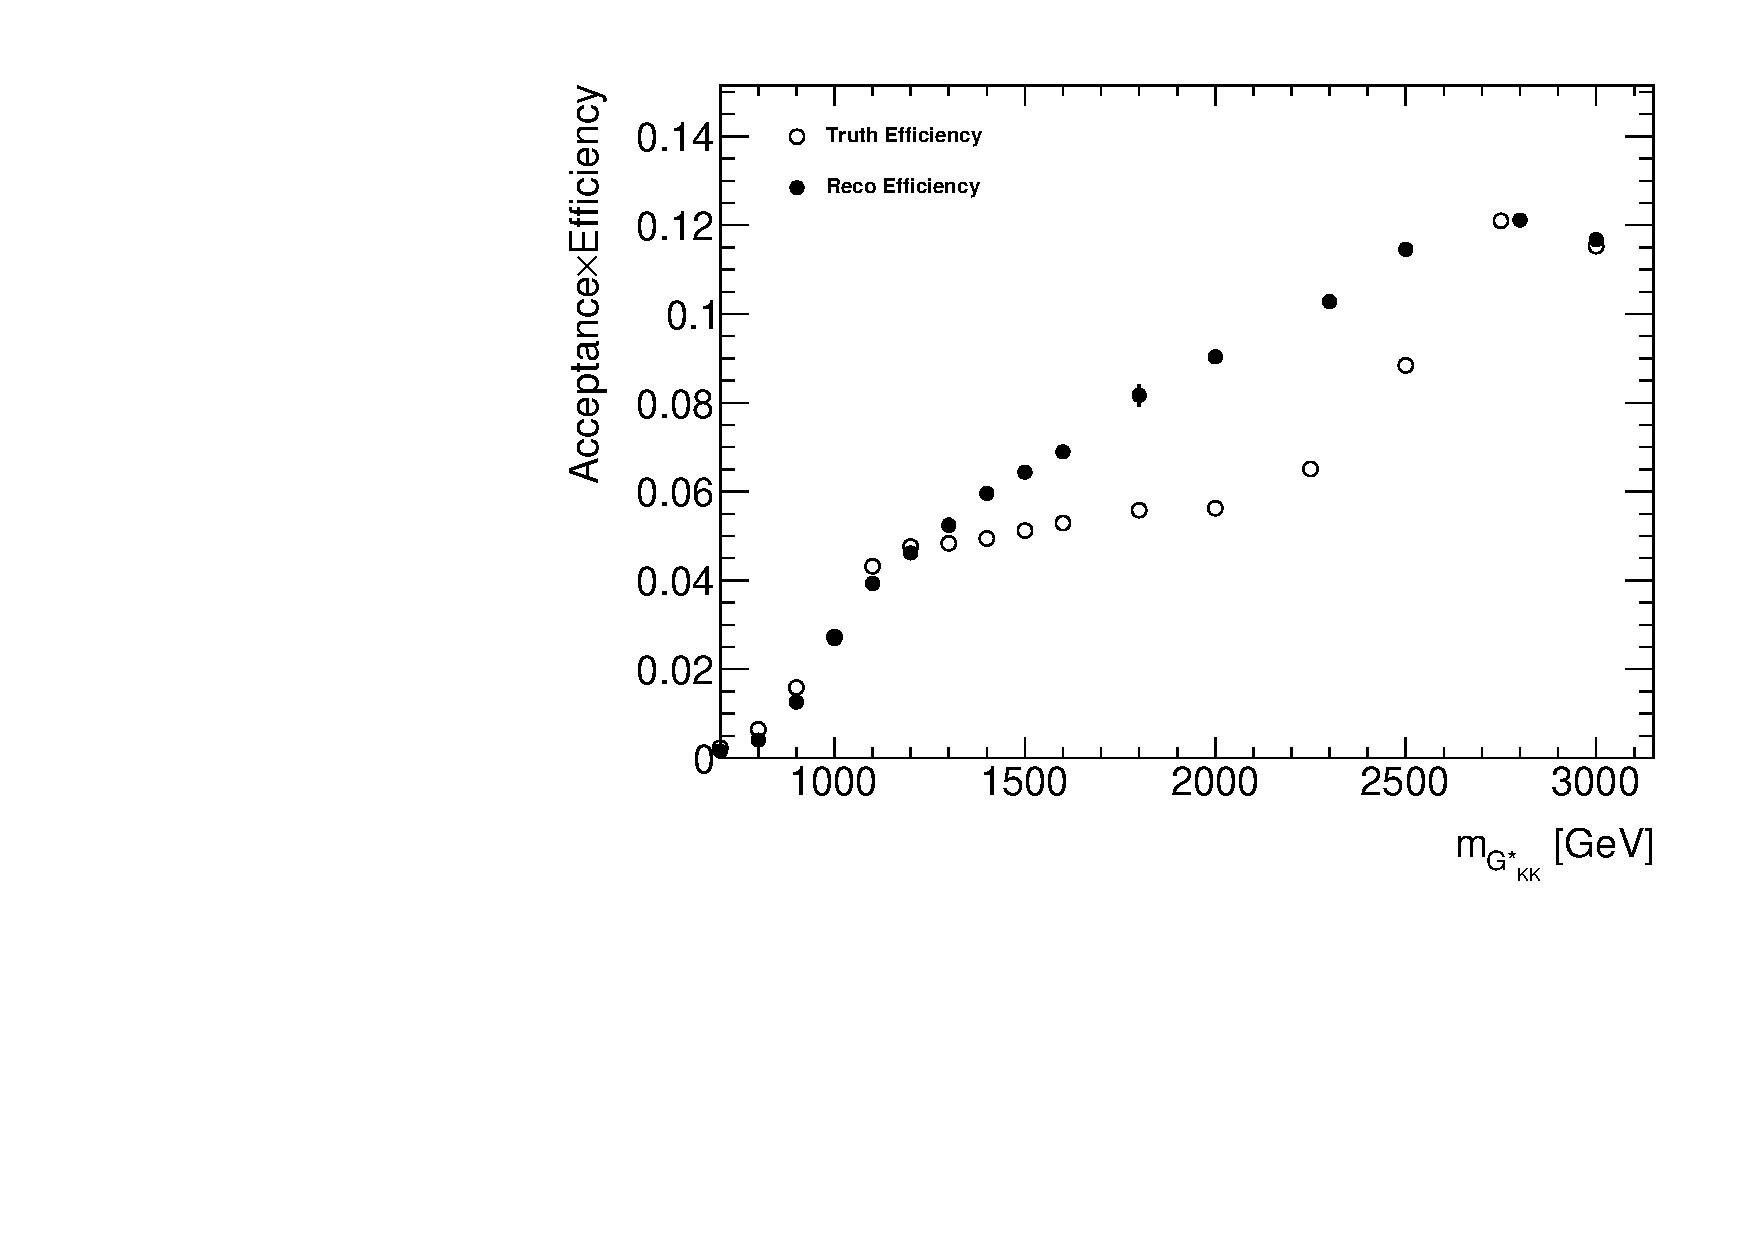
\includegraphics[width=0.3\textwidth, clip]{figures/boosted/Syst_MC/Boosted_2Tag_BulkRSGKKc1TruthVsReco.pdf}\hspace{5mm}}
% \subfloat[]{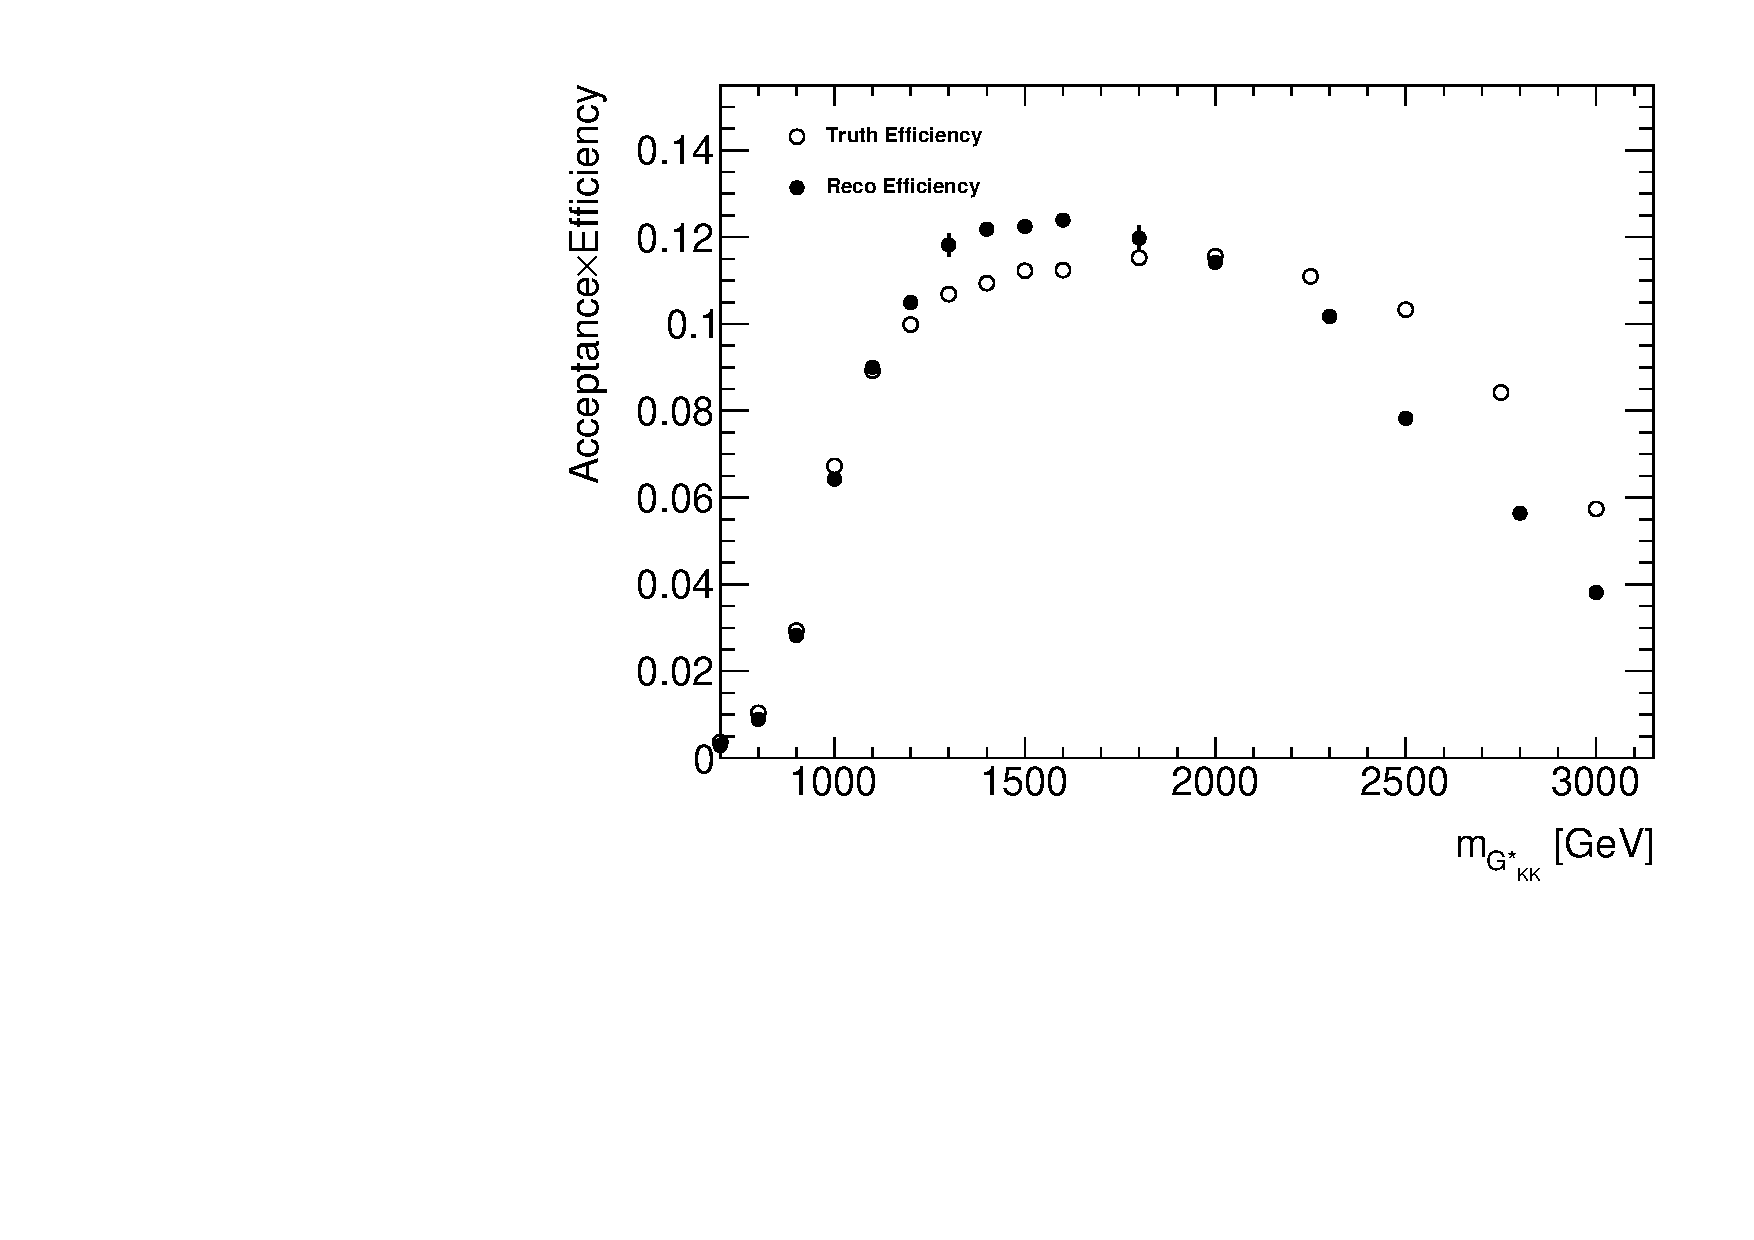
\includegraphics[width=0.3\textwidth, clip]{figures/boosted/Syst_MC/Boosted_3Tag_BulkRSGKKc1TruthVsReco.pdf}\hspace{5mm}}
% \subfloat[]{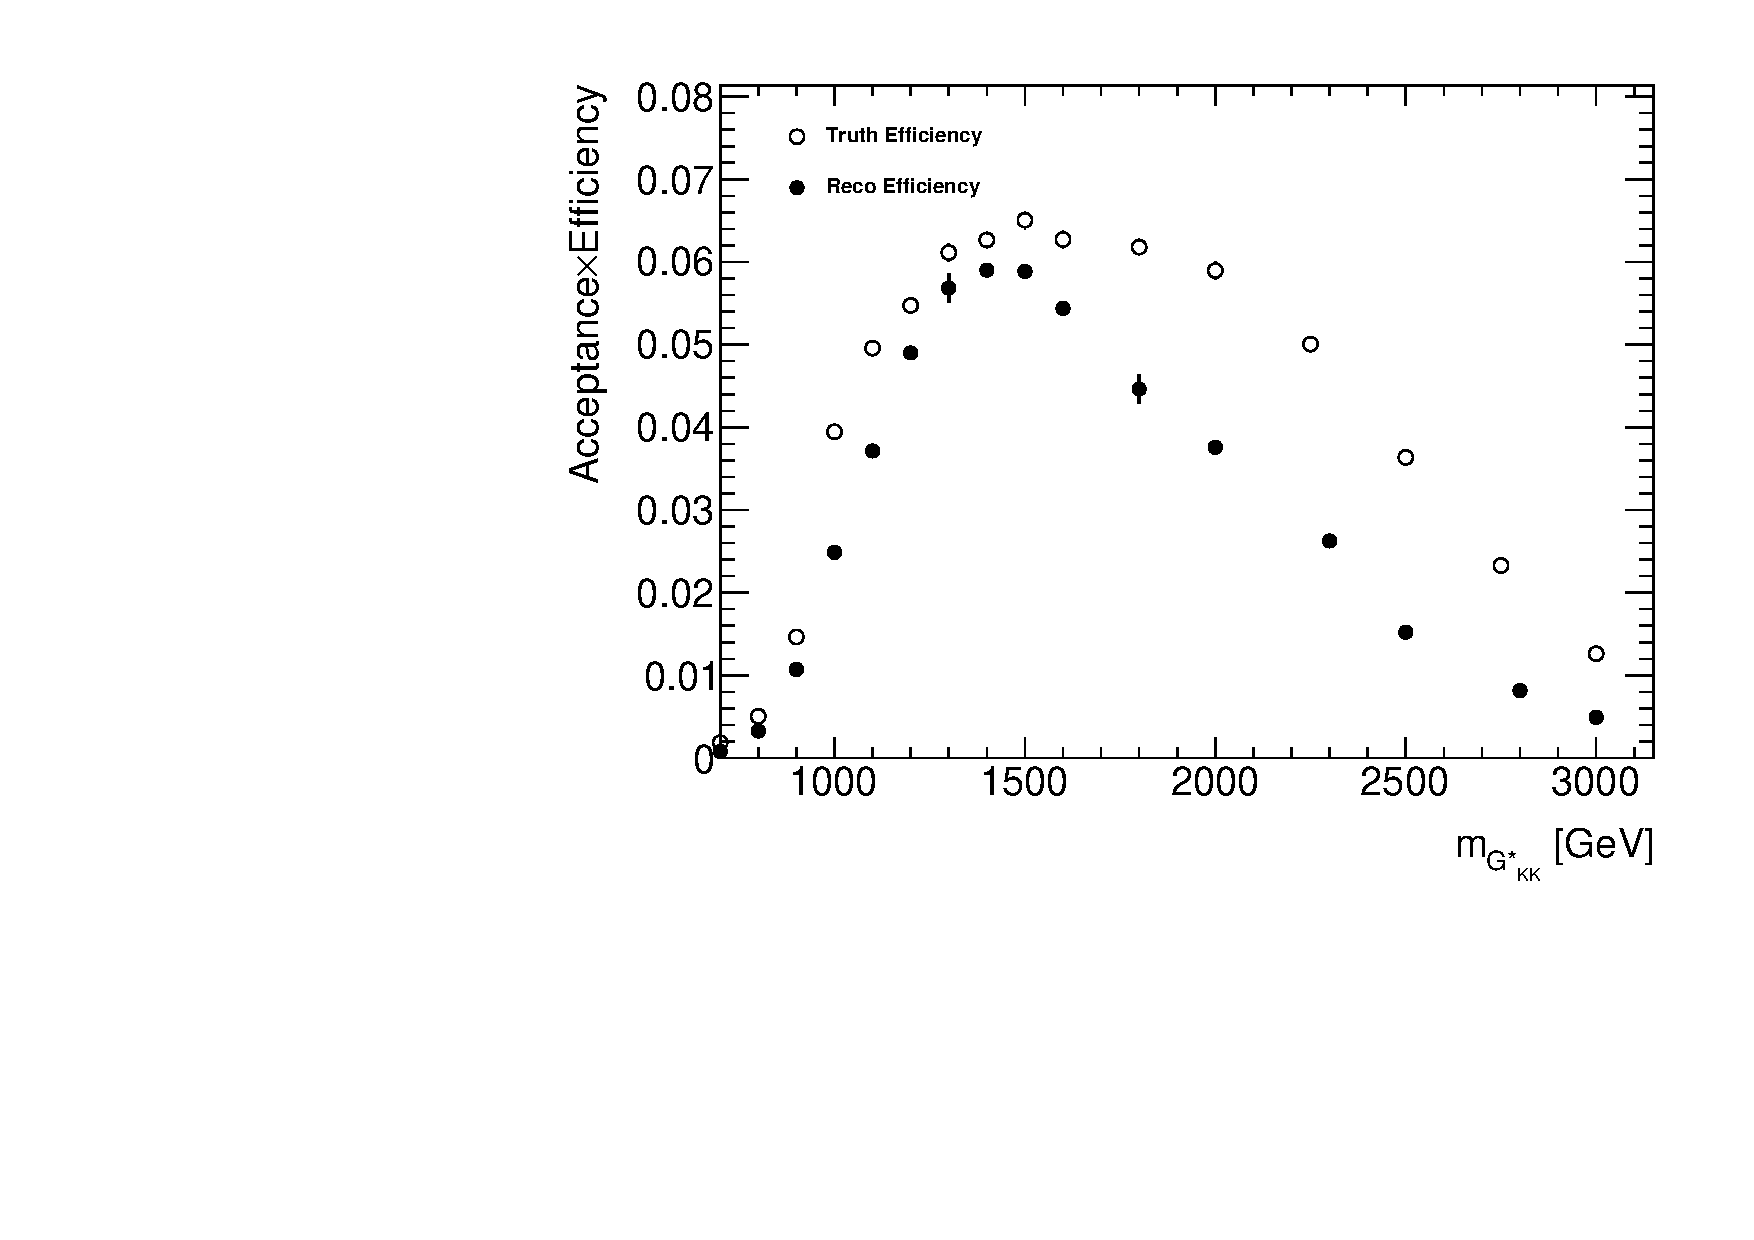
\includegraphics[width=0.3\textwidth, clip]{figures/boosted/Syst_MC/Boosted_4Tag_BulkRSGKKc1TruthVsReco.pdf}\hspace{5mm}}
% \caption{Acceptance times efficiency measured in the particle-level analysis (open circles) and full, reconstruction-level analysis (filled circles) for the graviton in the Bulk-RS model with $c=1$. (a) shows the 2-tag-split selection; (b) shows the 3-tag selection; and (c) shows the 4-tag selection}
% \label{fig:AccxEff_truthVsReco}
% \end{center}
% \end{figure*}

%%\paragraph{}
To evaluate the potential effect of missing higher order terms in the matrix element, the renormalisation and factorisation scales used in the signal generation were varied coherently by factors of $0.5\times$ and $2\times$ for the signals. The effect is shown as function of resonance mass in Figure \ref{fig:scaleVar}.

% \begin{figure*}
% \begin{center}
% \subfloat[2-Tag-Split: bulk RS c=1]{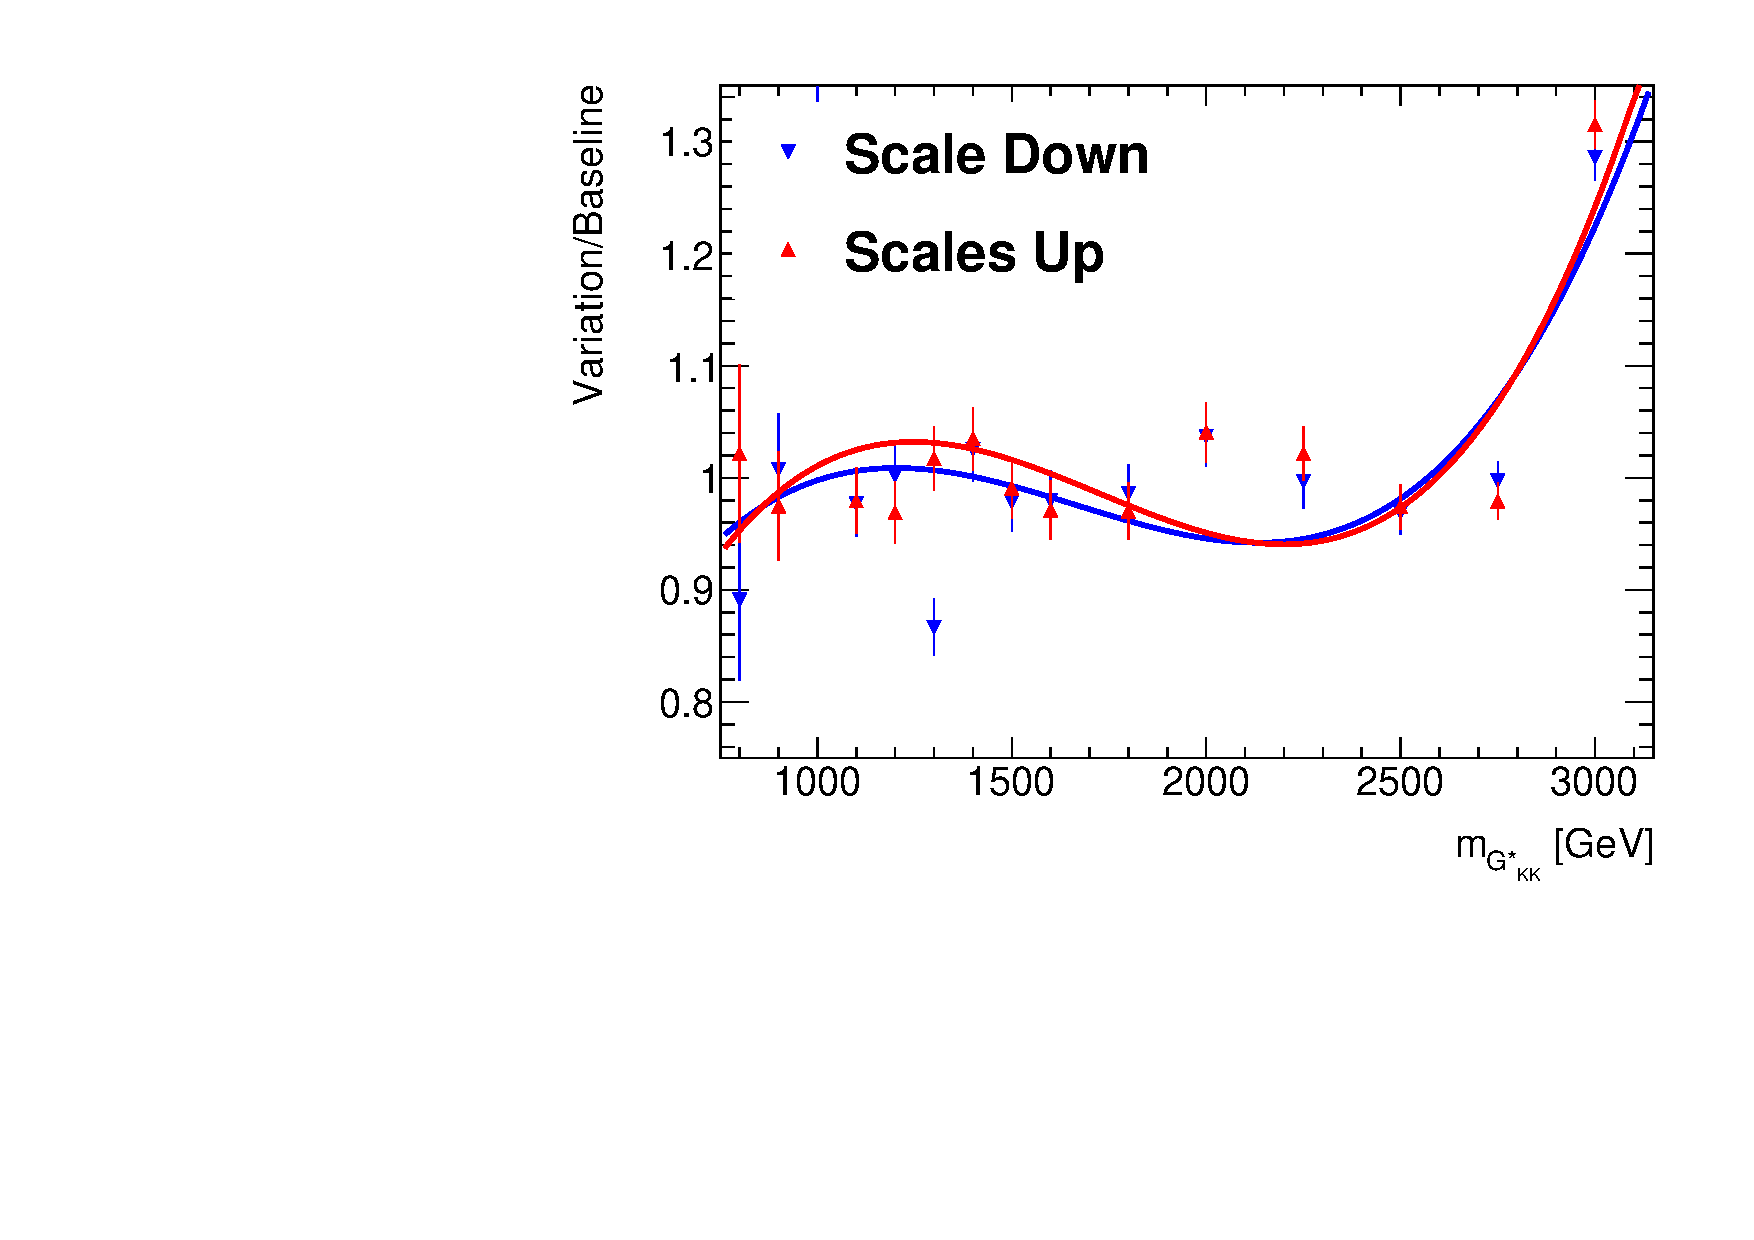
\includegraphics[width=0.3\textwidth, clip]{figures/boosted/Syst_MC/Boosted_2Tag_BulkRSGKKc1_Scale_ratio.pdf}\hspace{5mm}}
% \subfloat[2-Tag-Split: bulk RS c=2]{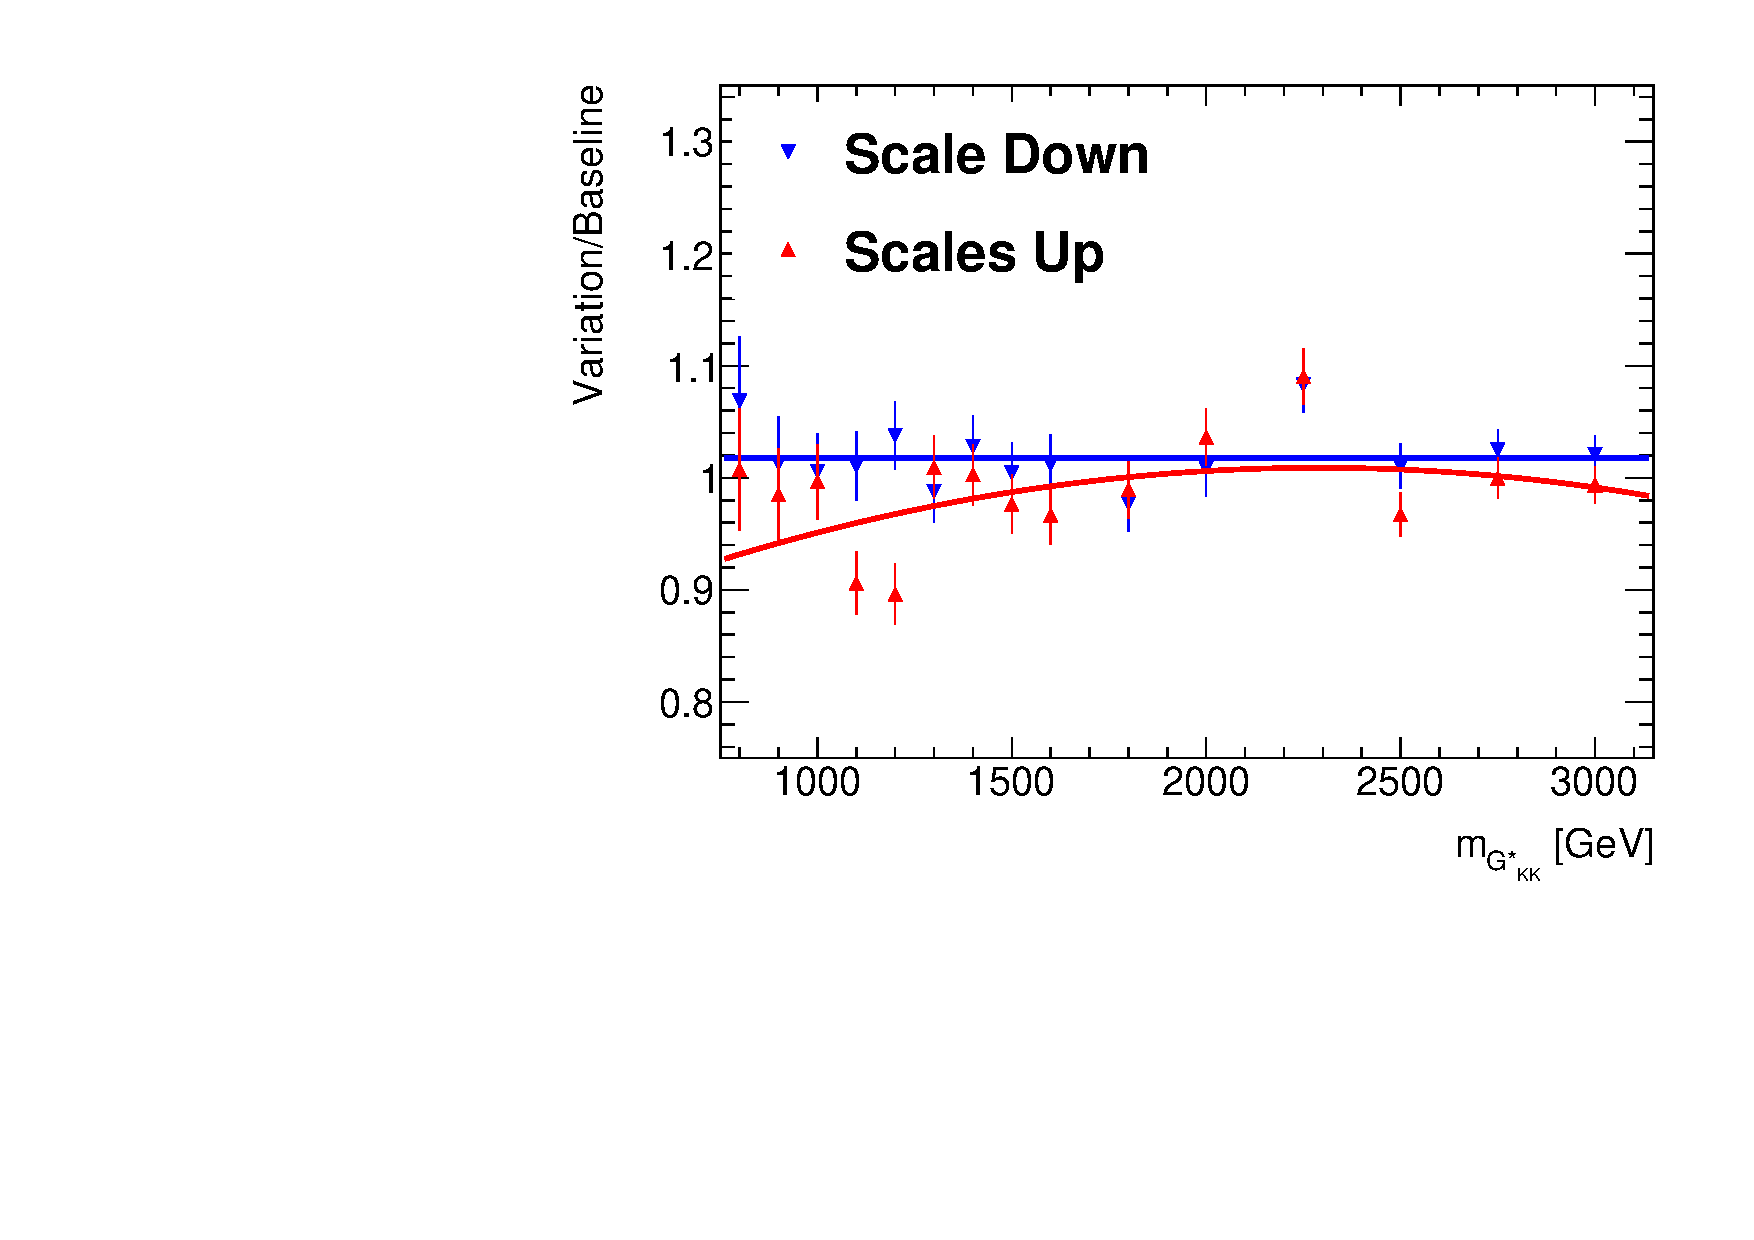
\includegraphics[width=0.3\textwidth, clip]{figures/boosted/Syst_MC/Boosted_2Tag_BulkRSGKKc2_Scale_ratio.pdf}\hspace{5mm}}
% \subfloat[2-Tag-Split: scalar]{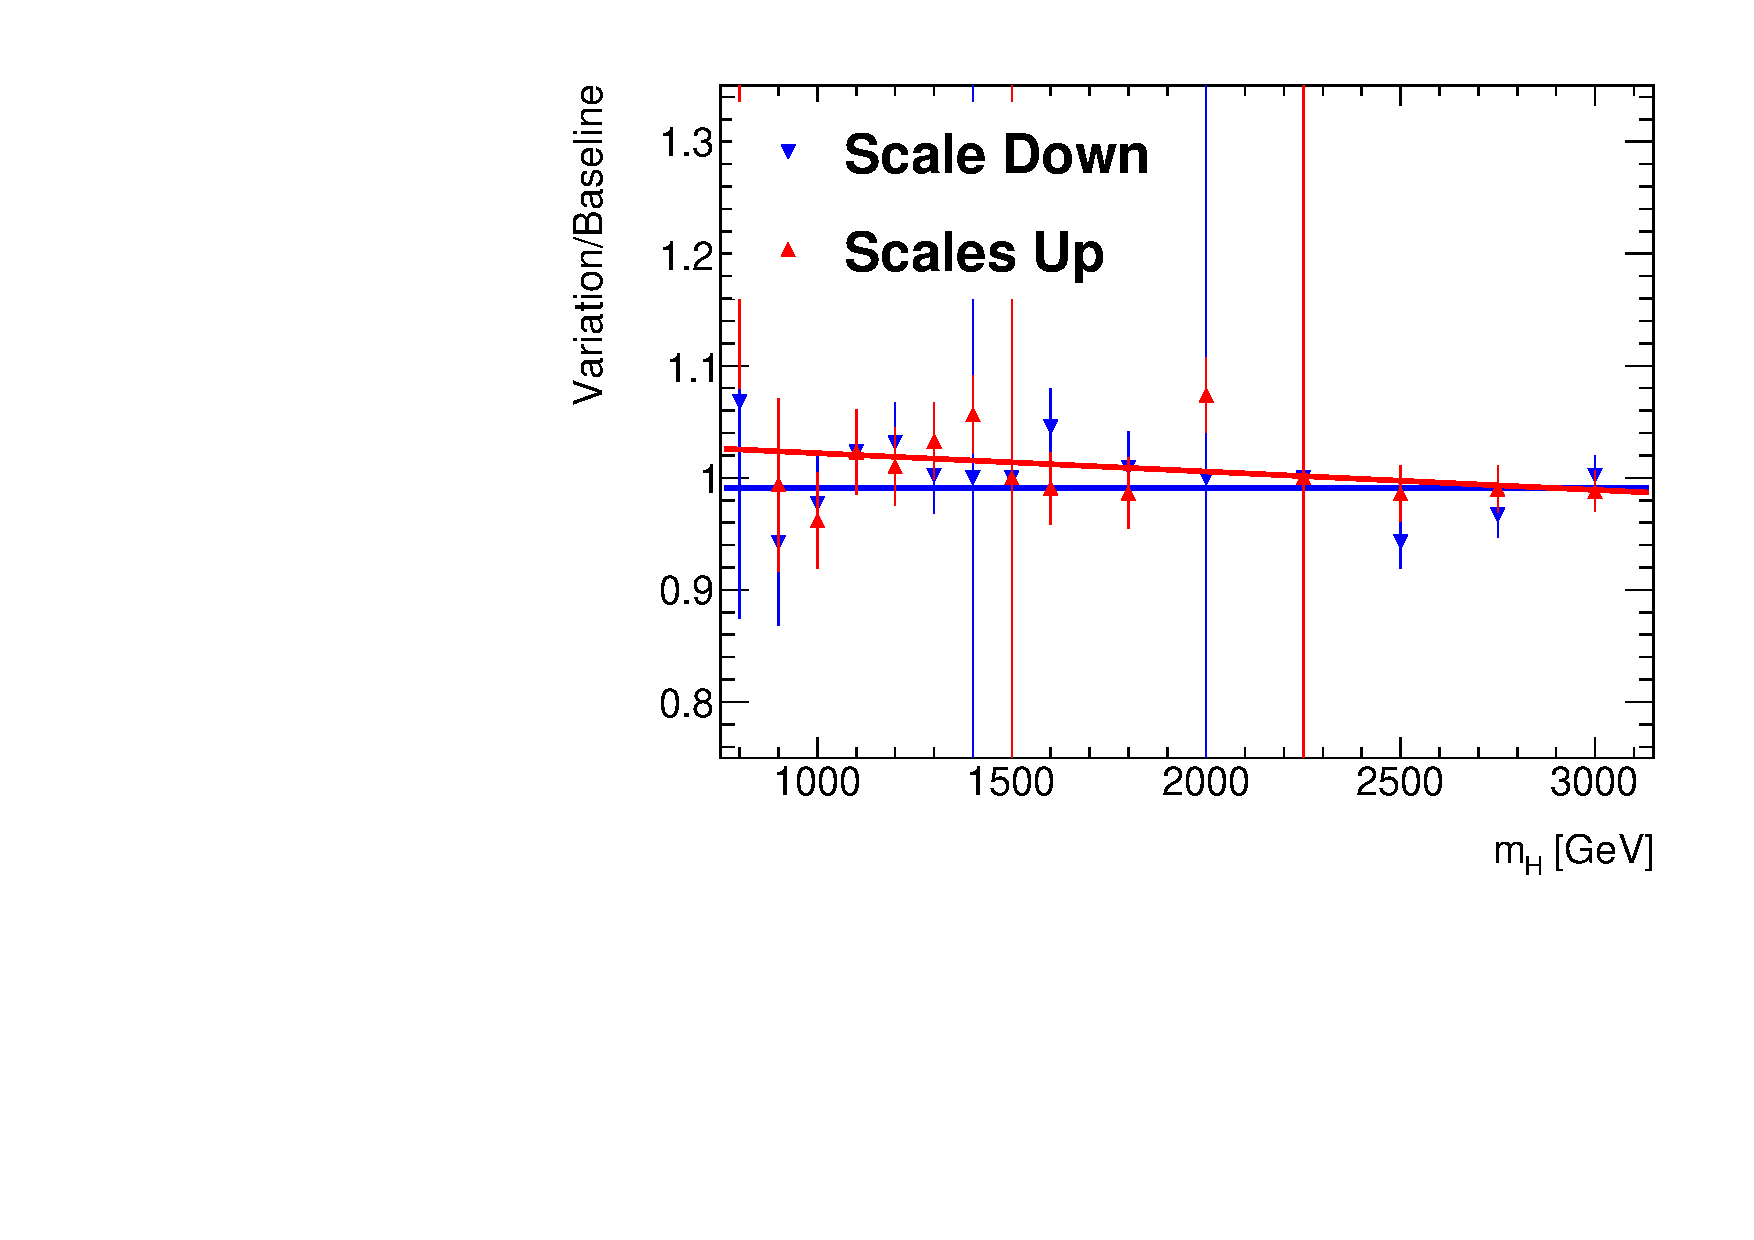
\includegraphics[width=0.3\textwidth, clip]{figures/boosted/Syst_MC/Boosted_2Tag_Scalar_Scale_ratio.pdf}\hspace{5mm}}\\
% \subfloat[3-Tag: bulk RS c=1]{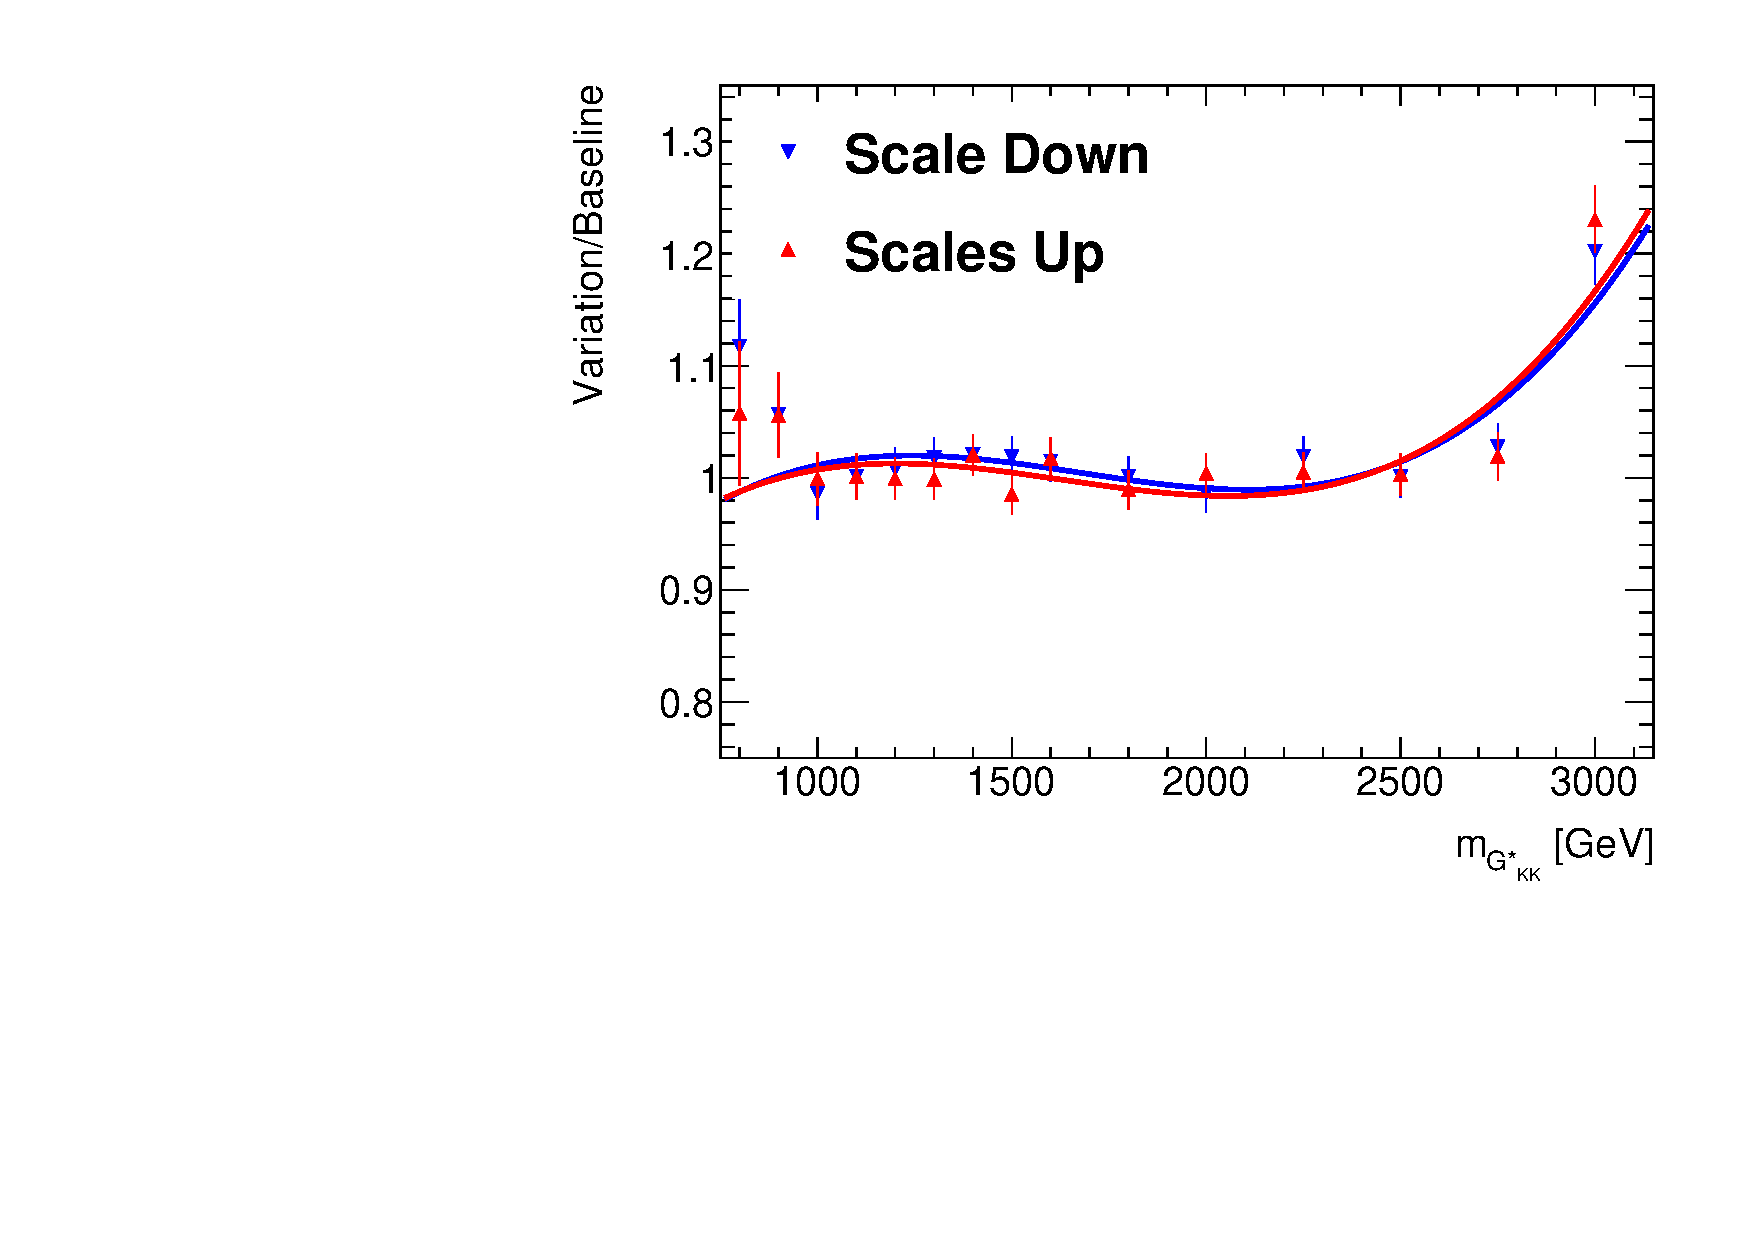
\includegraphics[width=0.3\textwidth, clip]{figures/boosted/Syst_MC/Boosted_3Tag_BulkRSGKKc1_Scale_ratio.pdf}\hspace{5mm}}
% \subfloat[3-Tag: bulk RS c=2]{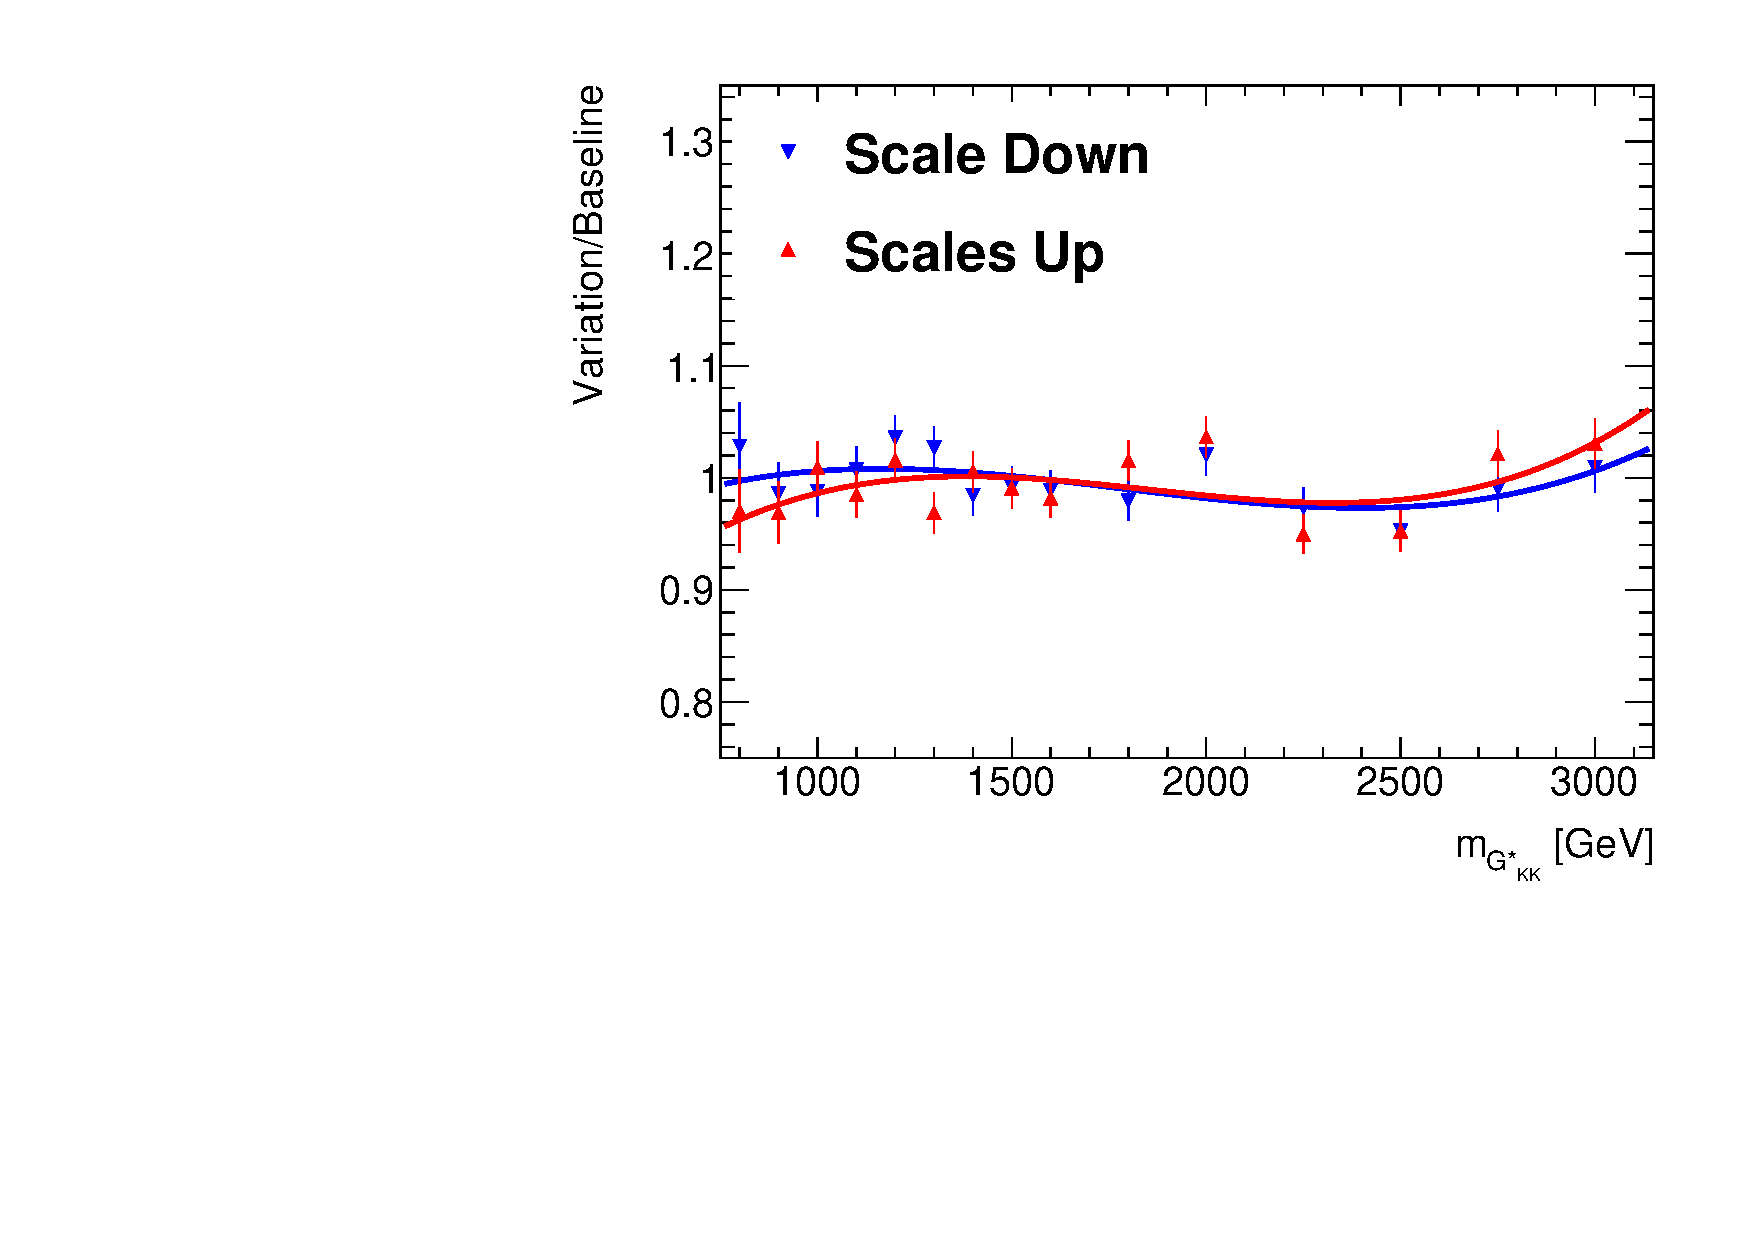
\includegraphics[width=0.3\textwidth, clip]{figures/boosted/Syst_MC/Boosted_3Tag_BulkRSGKKc2_Scale_ratio.pdf}\hspace{5mm}}
% \subfloat[3-Tag: scalar]{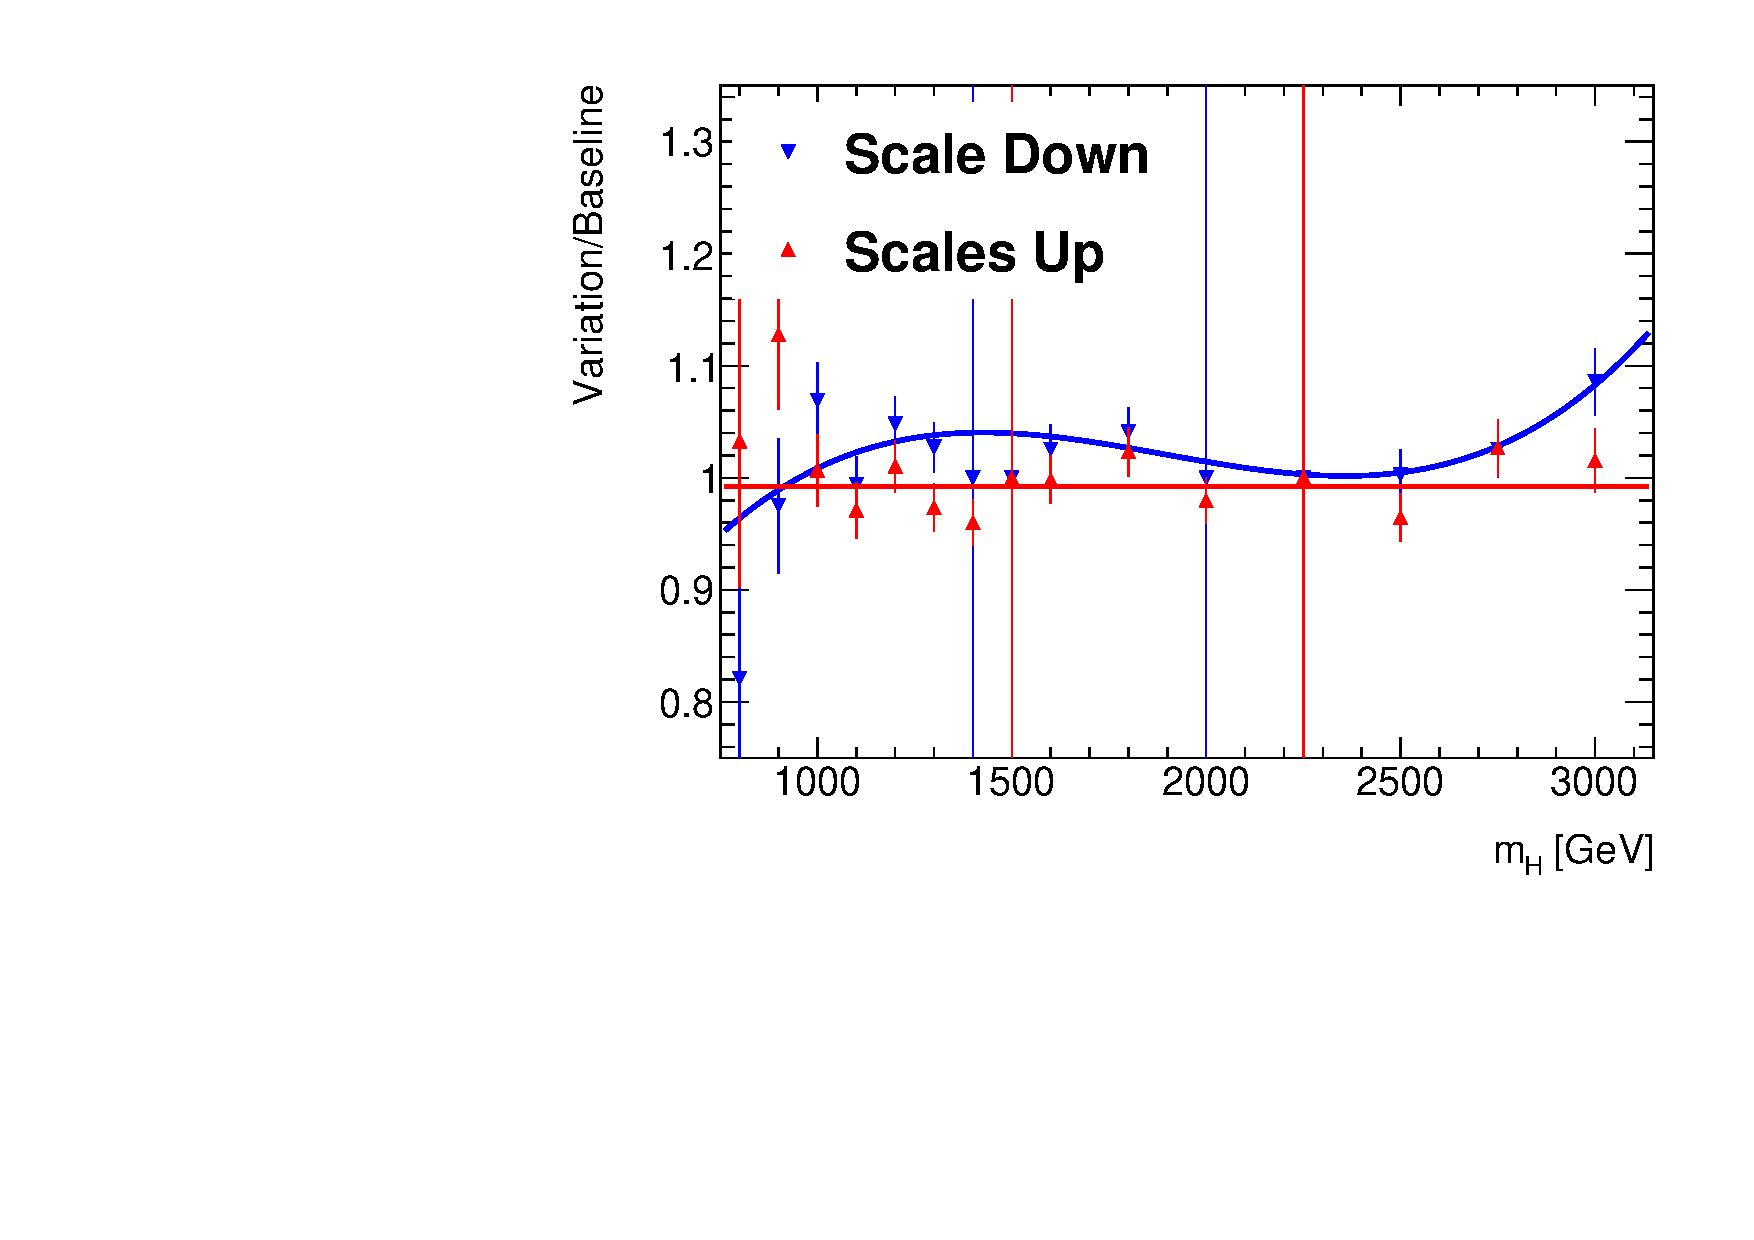
\includegraphics[width=0.3\textwidth, clip]{figures/boosted/Syst_MC/Boosted_3Tag_Scalar_Scale_ratio.pdf}\hspace{5mm}}\\
% \subfloat[4-Tag: bulk RS c=1]{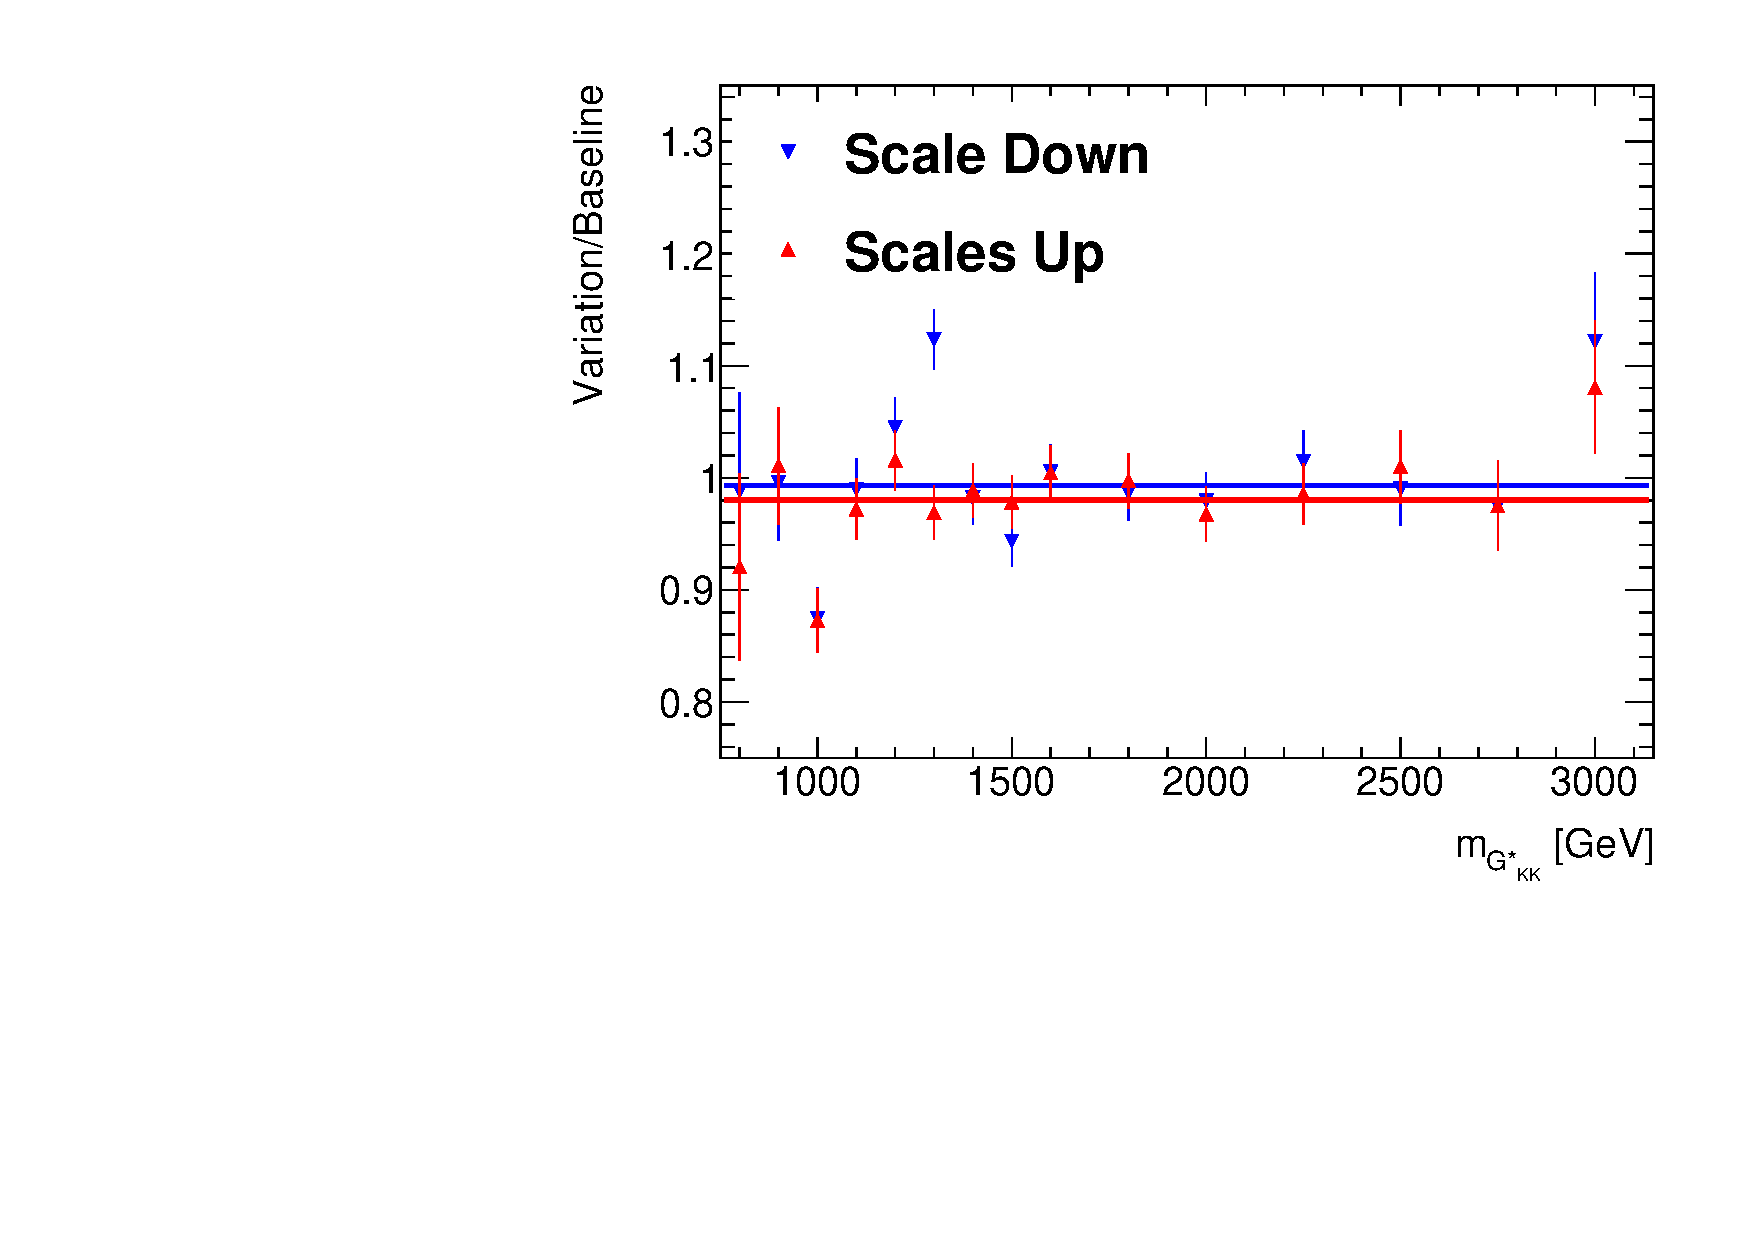
\includegraphics[width=0.3\textwidth, clip]{figures/boosted/Syst_MC/Boosted_4Tag_BulkRSGKKc1_Scale_ratio.pdf}\hspace{5mm}}
% \subfloat[4-Tag: bulk RS c=2]{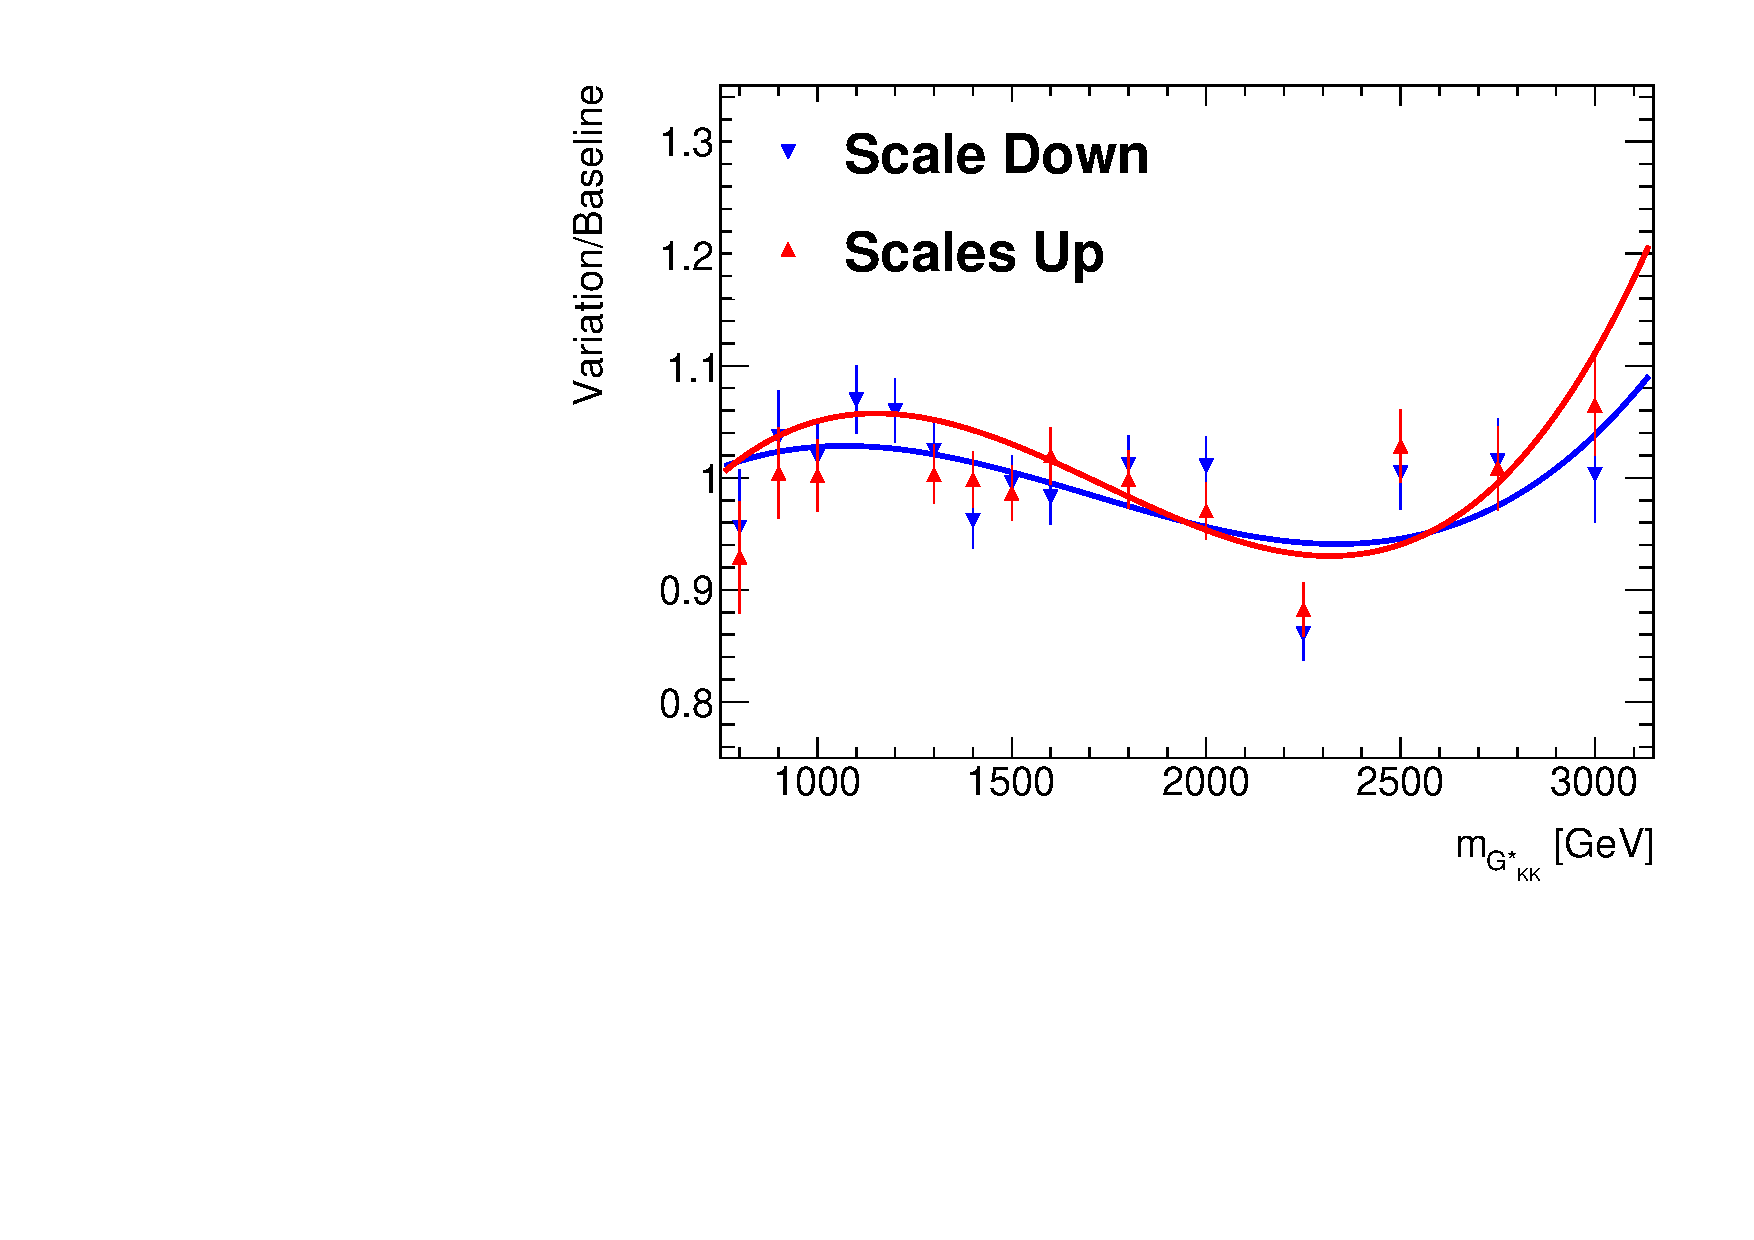
\includegraphics[width=0.3\textwidth, clip]{figures/boosted/Syst_MC/Boosted_4Tag_BulkRSGKKc2_Scale_ratio.pdf}\hspace{5mm}}
% \subfloat[4-Tag: scalar]{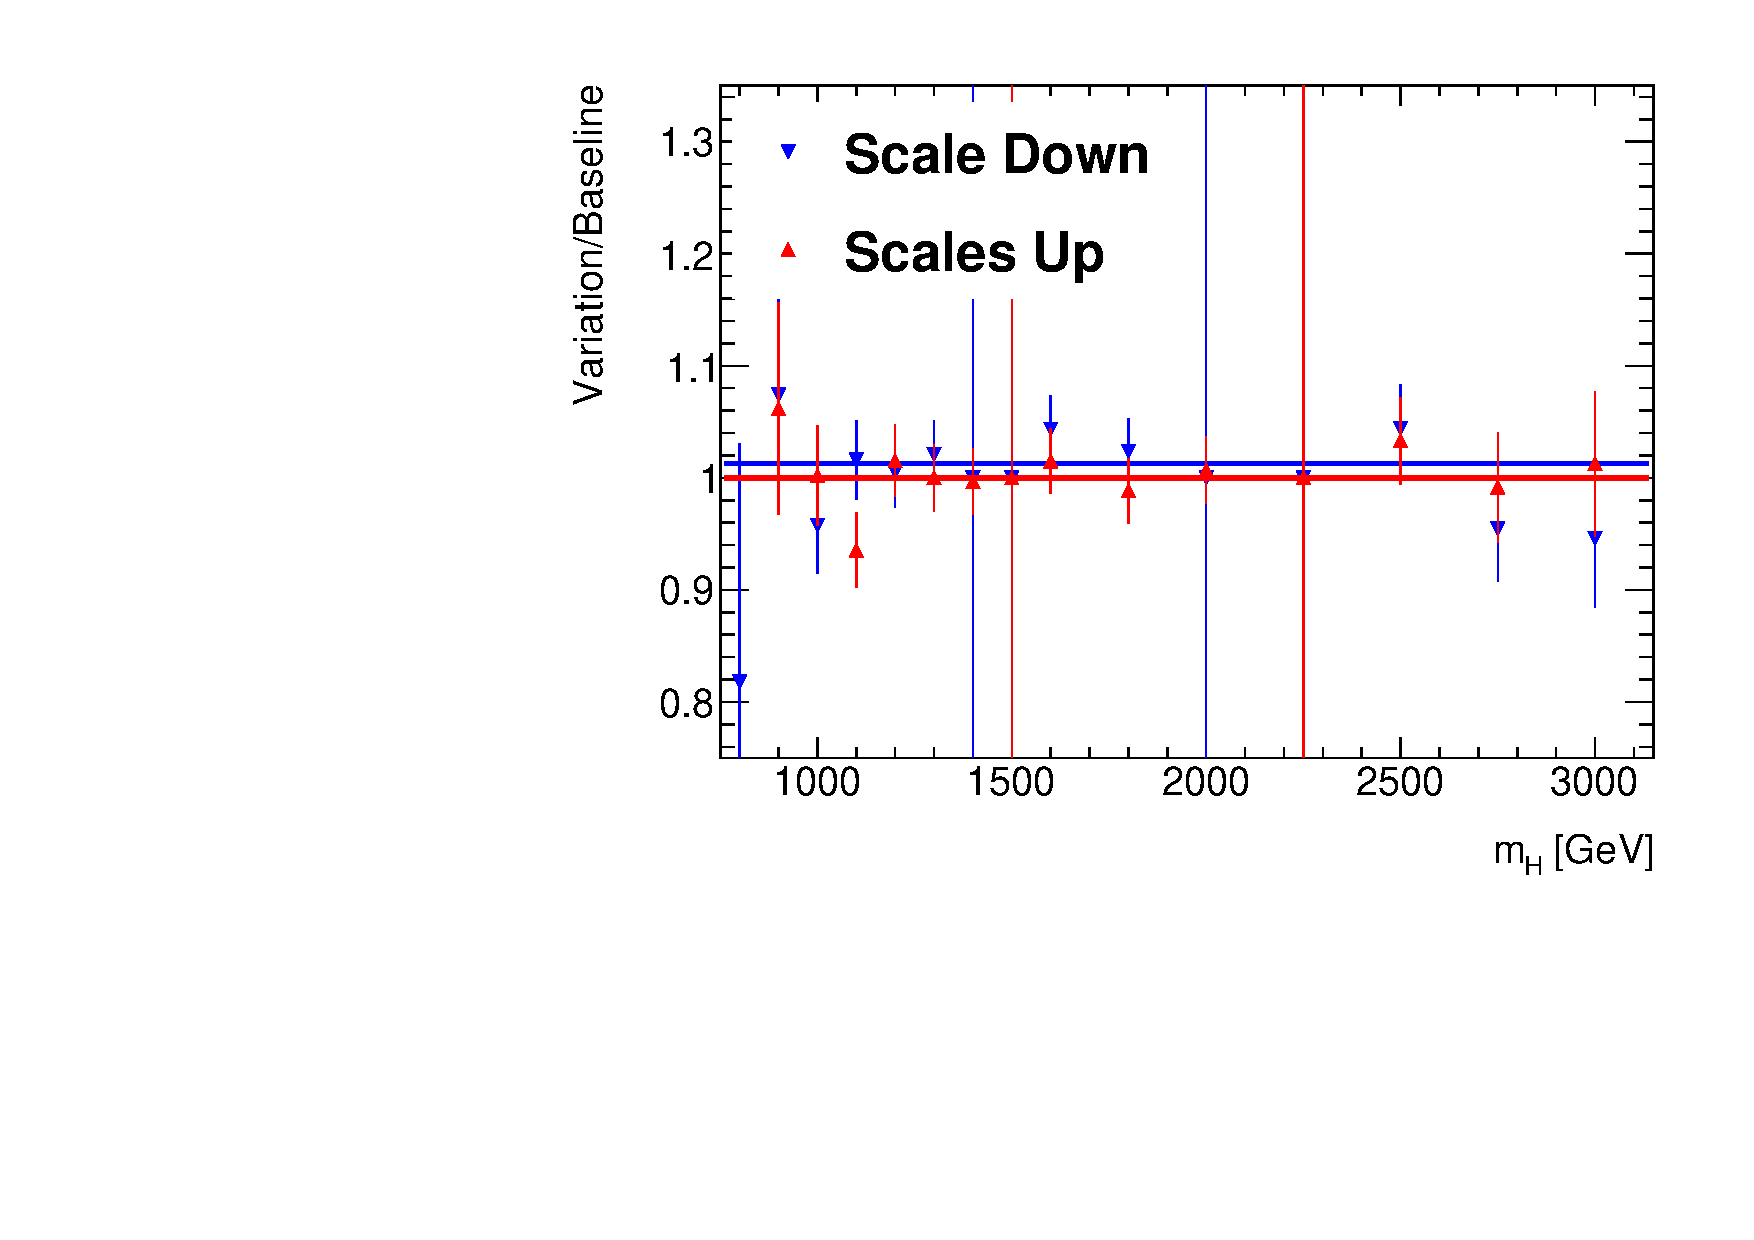
\includegraphics[width=0.3\textwidth, clip]{figures/boosted/Syst_MC/Boosted_4Tag_Scalar_Scale_ratio.pdf}\hspace{5mm}}
% \caption{Ratio of acceptance times efficiency measured in the scale-varied samples over the baseline sample. The upward-pointing triangles correspond to doubling both the renormalisation and factorisation scales, while the downward-pointing triangles correspond to halving them. The polynomial fits shown as solid lines are used to assign the corresponding systematic variation in the final statistical analysis.}
% \label{fig:scaleVar}
% \end{center}
% \end{figure*}

%\paragraph{}
Uncertainties due to modelling of the parton shower and the underlying event (including multi-parton interactions) are evaluated by switching the MC generator used. For the Bulk RS graviton samples, this means switching from Pythia 8 to Herwig++, while for the scalar and non-resonant it is Herwig++ to Pythia 8. Figure \ref{fig:showerVar} shows the impact of these variations on the signal acceptance.

% \begin{figure*}
% \begin{center}
% \subfloat[2-Tag-Split: bulk RS c=1]{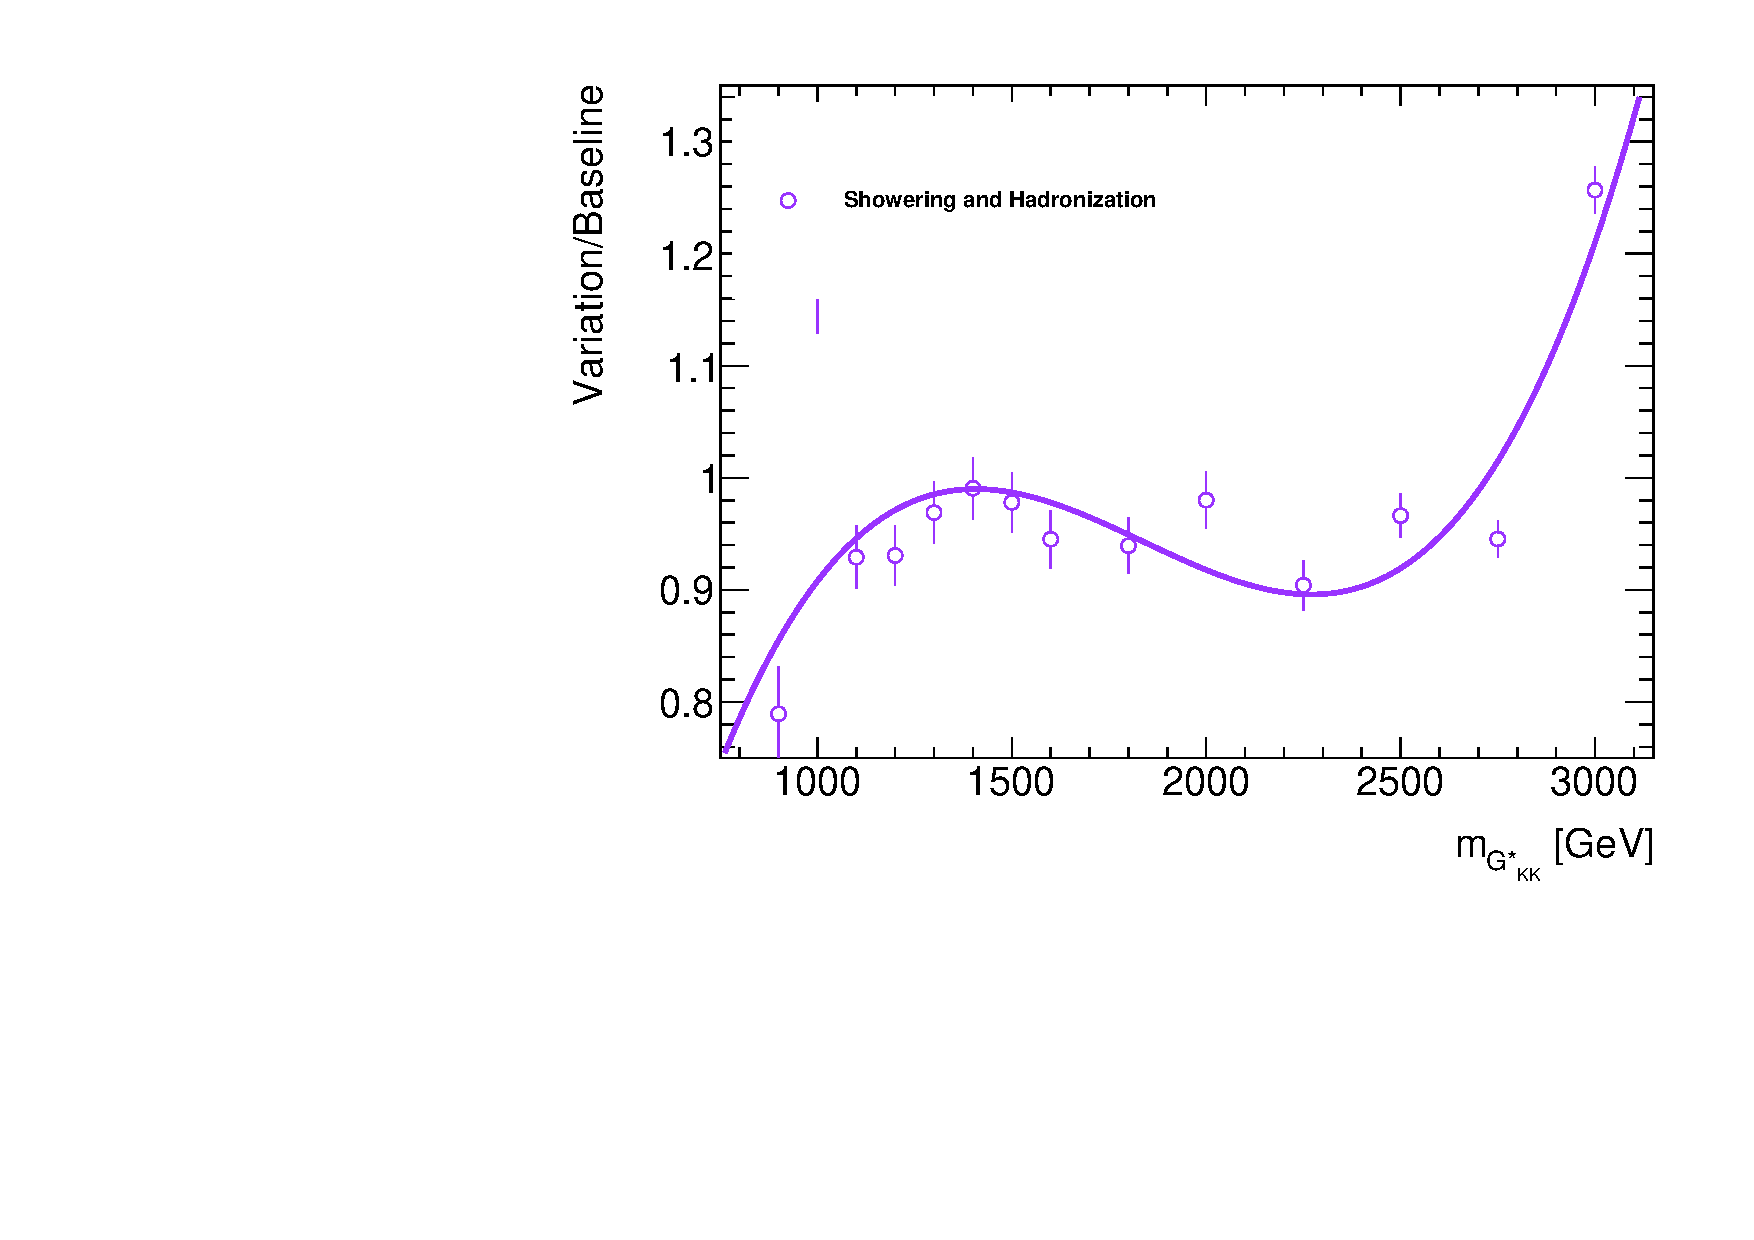
\includegraphics[width=0.3\textwidth, clip]{figures/boosted/Syst_MC/Boosted_2Tag_BulkRSGKKc1_Shower_ratio.pdf}\hspace{5mm}}
% \subfloat[2-Tag-Split: bulk RS c=2]{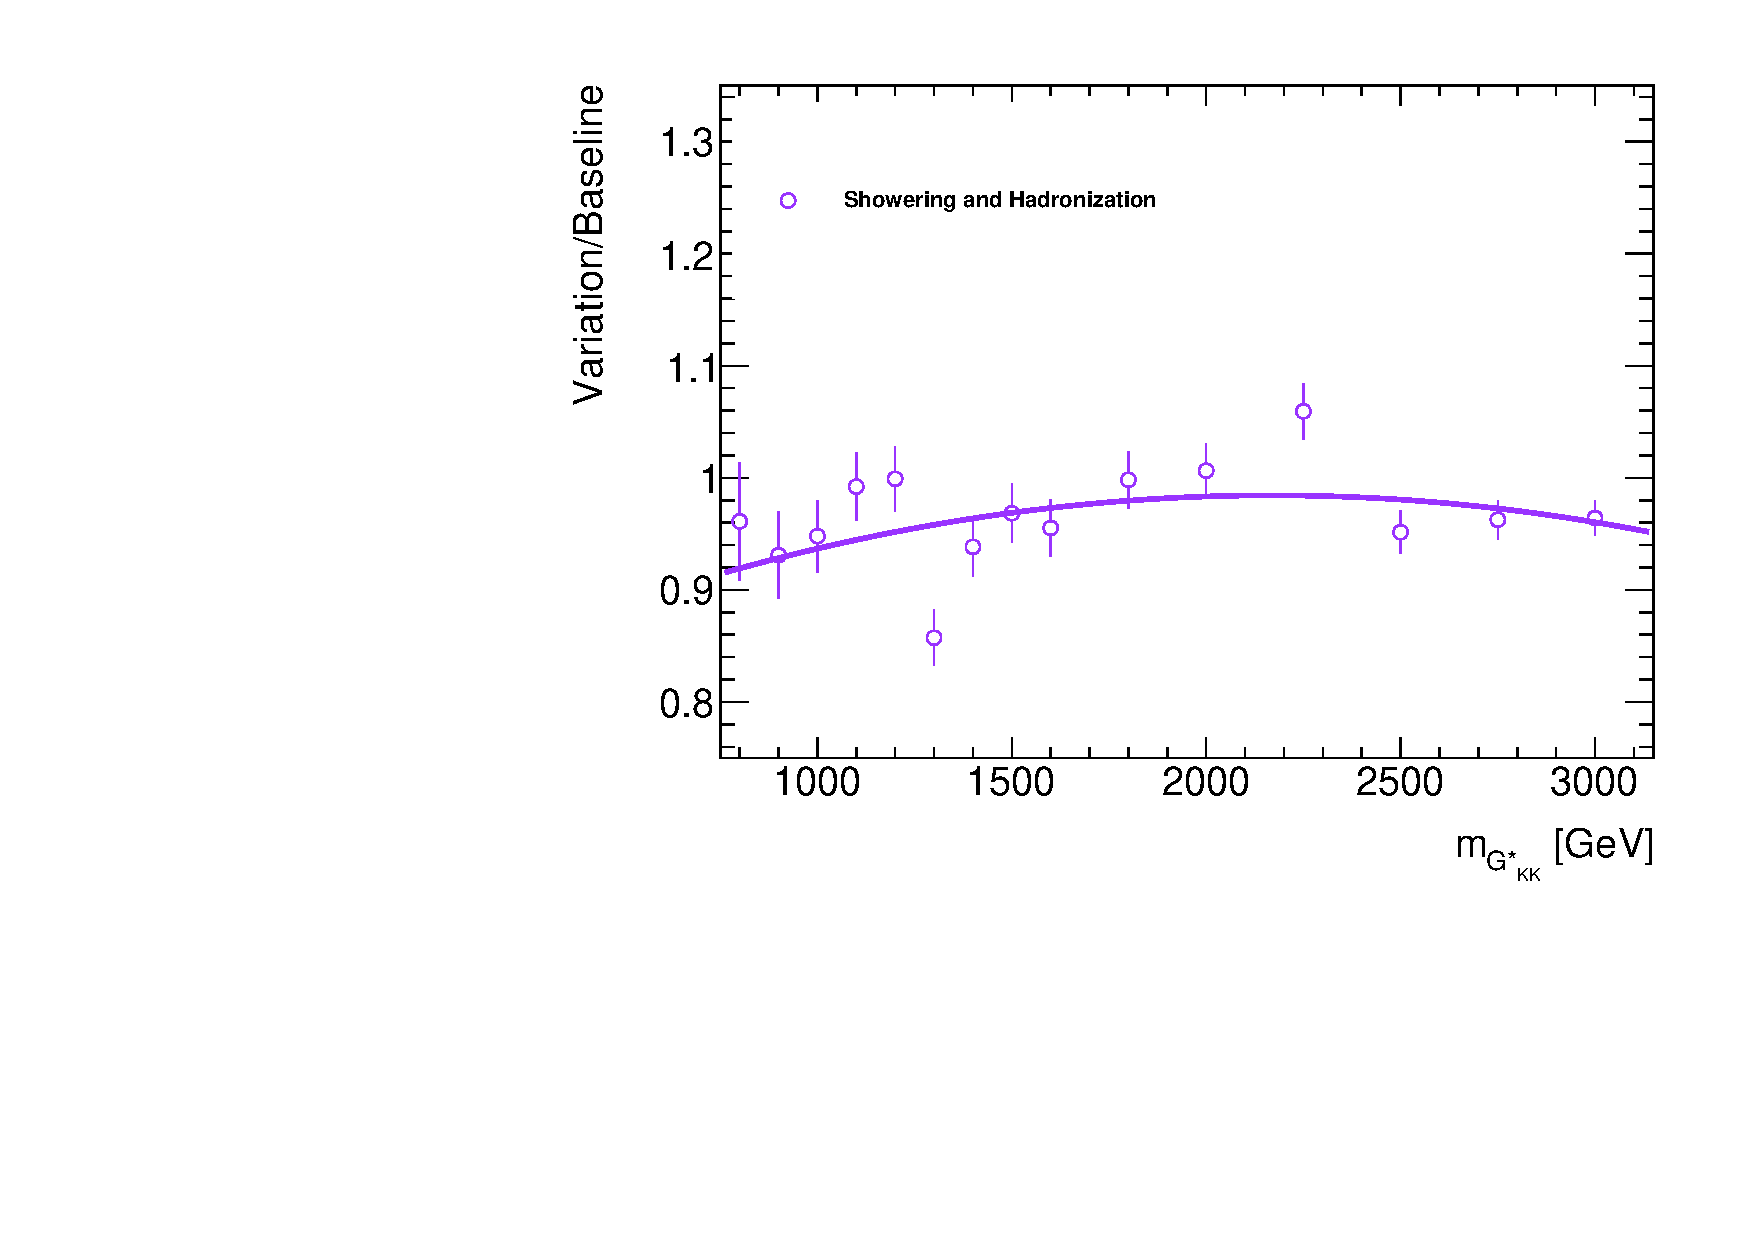
\includegraphics[width=0.3\textwidth, clip]{figures/boosted/Syst_MC/Boosted_2Tag_BulkRSGKKc2_Shower_ratio.pdf}\hspace{5mm}}
% \subfloat[2-Tag-Split: scalar]{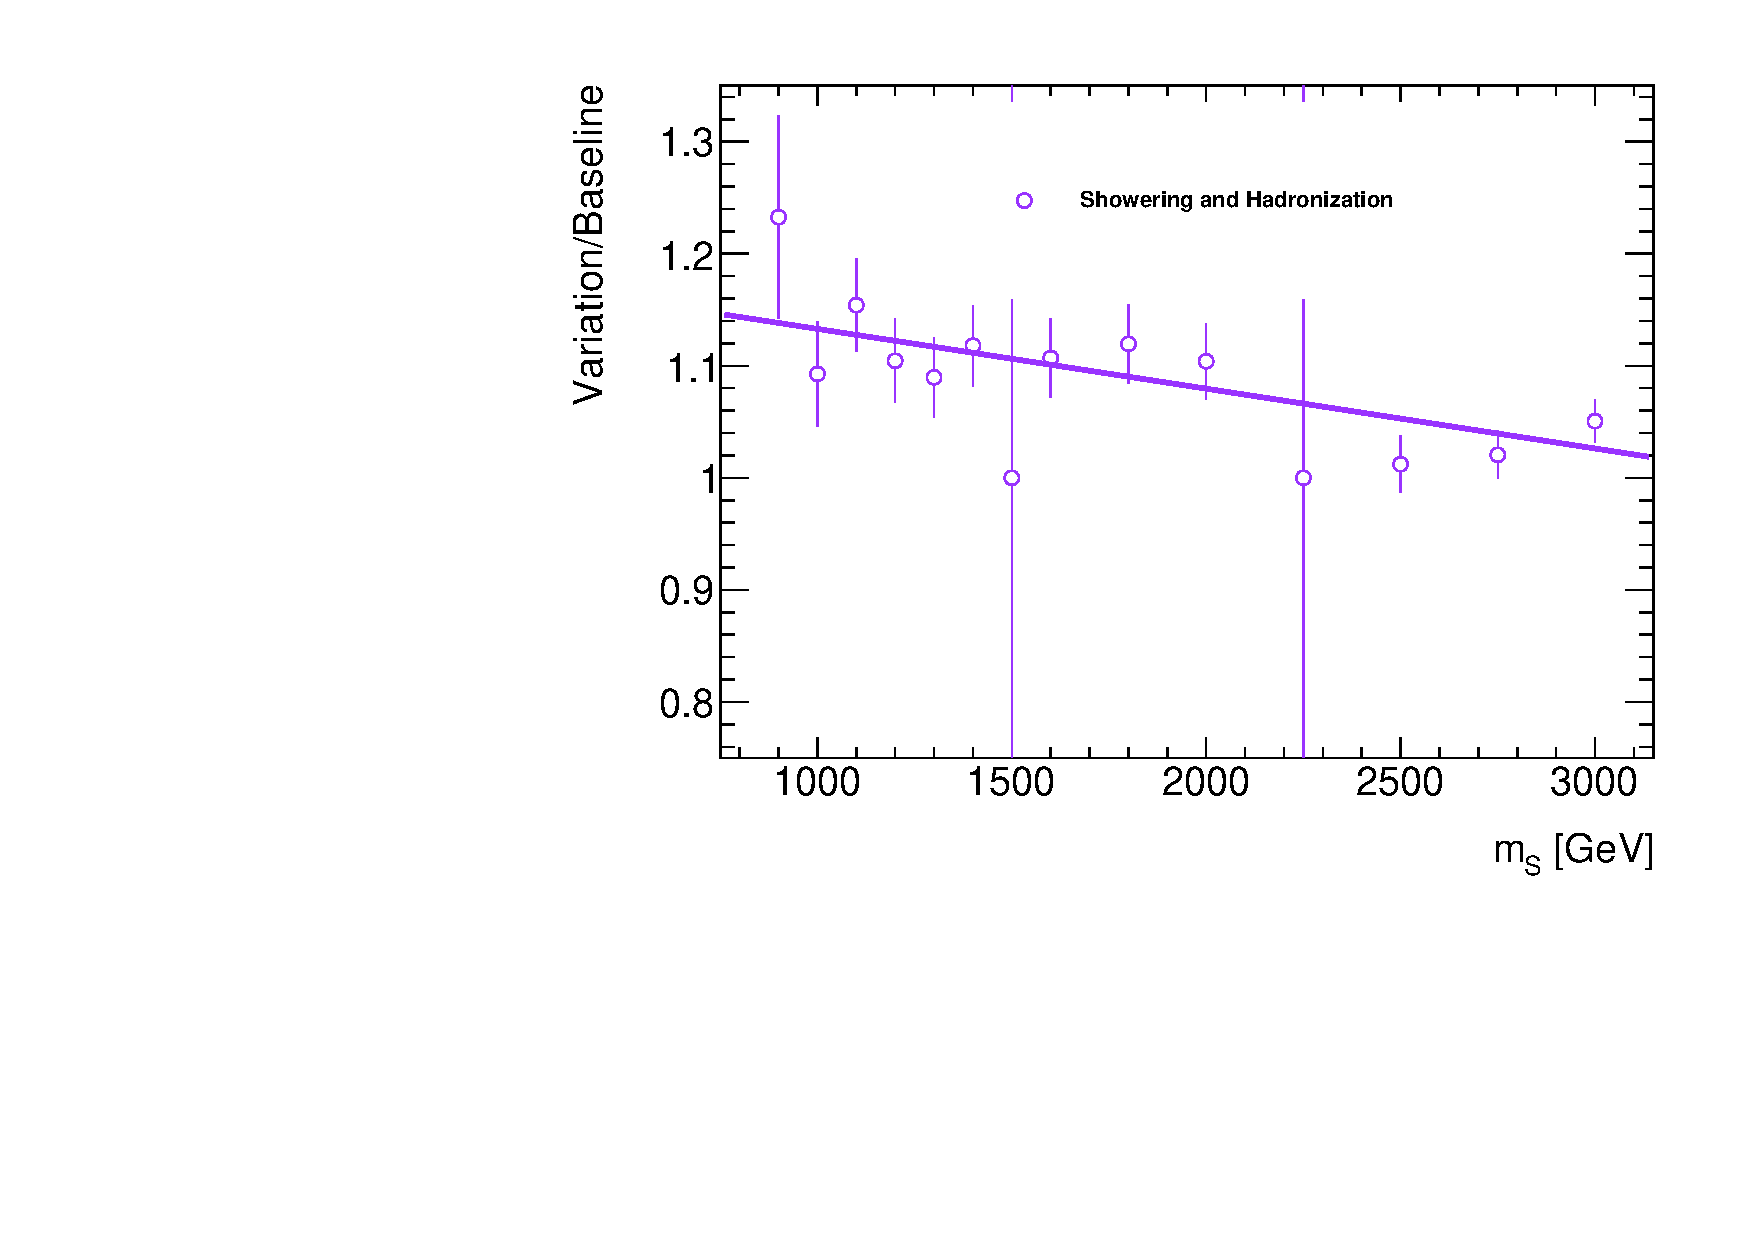
\includegraphics[width=0.3\textwidth, clip]{figures/boosted/Syst_MC/Boosted_2Tag_Scalar_Shower_ratio.pdf}\hspace{5mm}}\\
% \subfloat[3-Tag: bulk RS c=1]{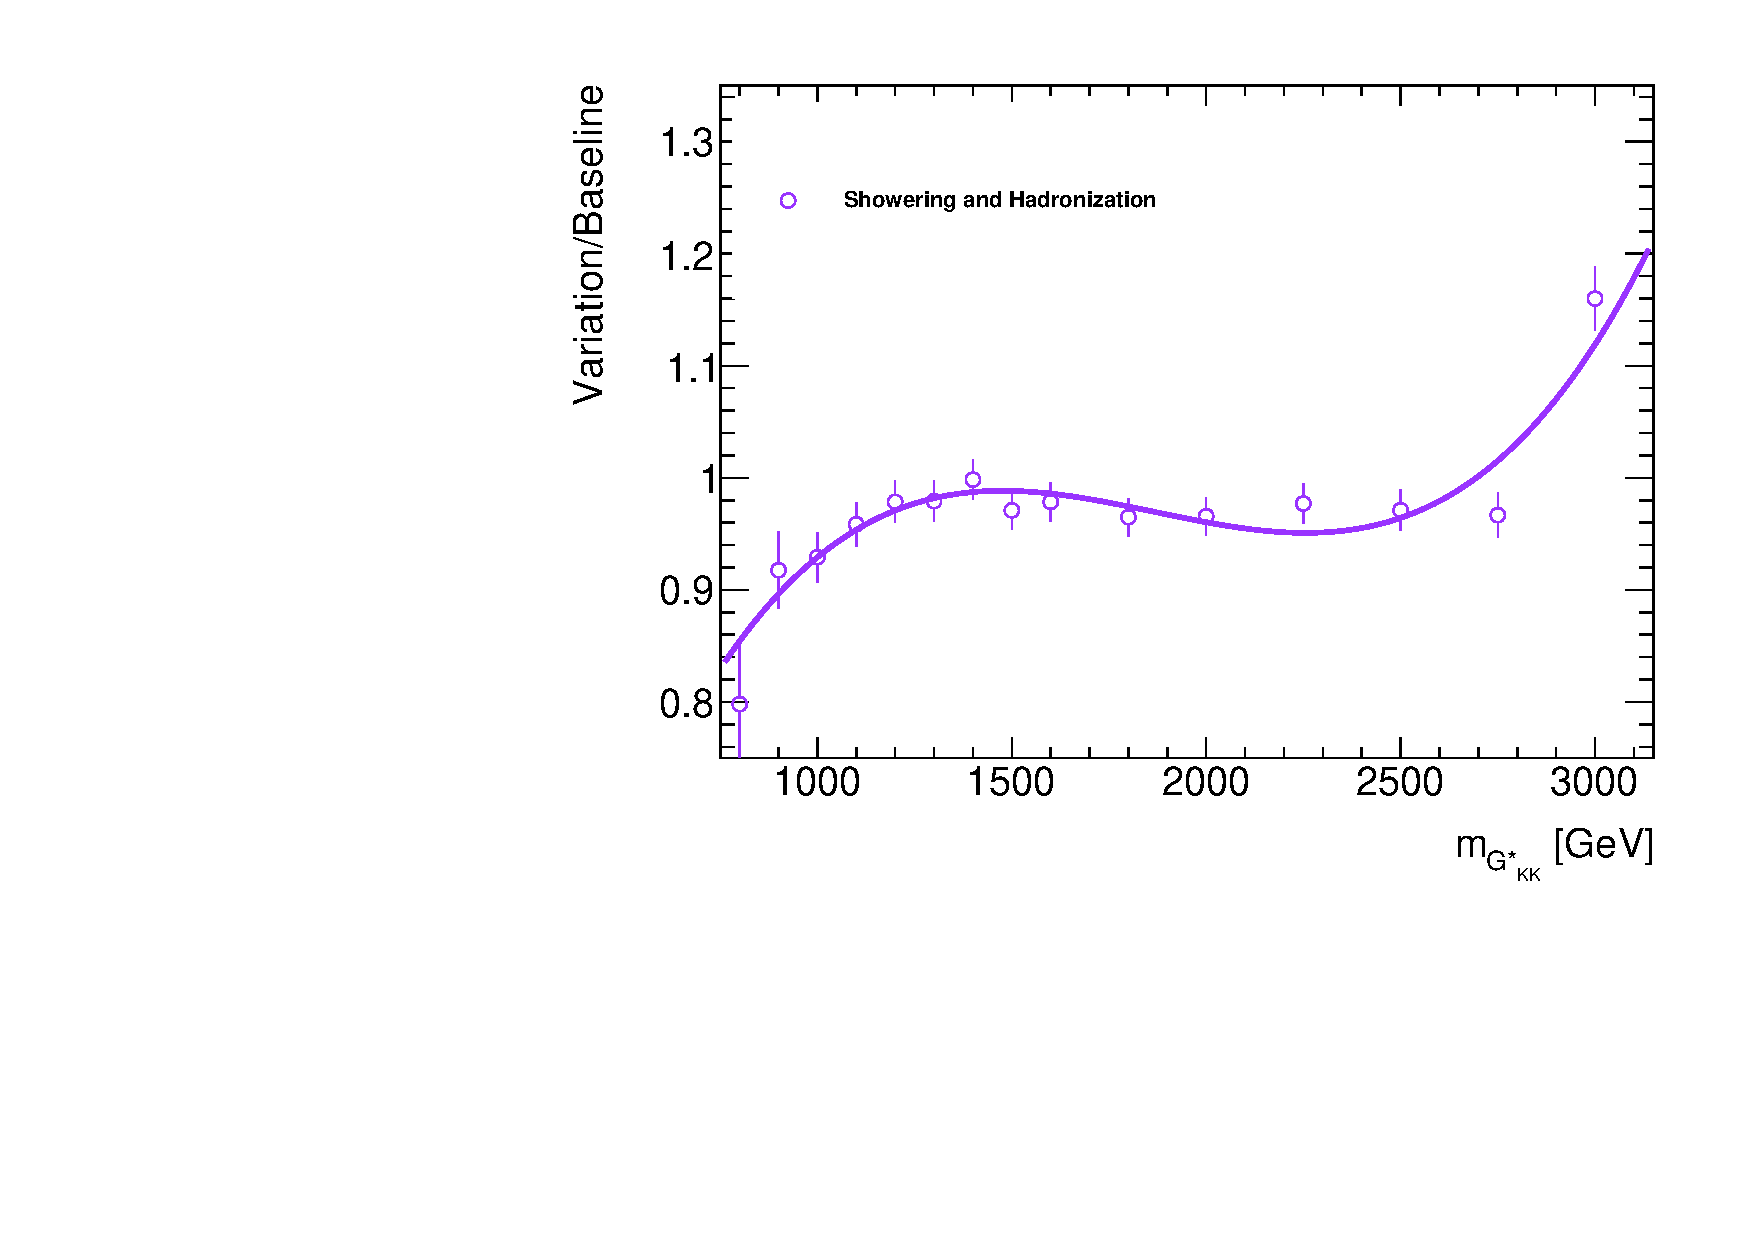
\includegraphics[width=0.3\textwidth, clip]{figures/boosted/Syst_MC/Boosted_3Tag_BulkRSGKKc1_Shower_ratio.pdf}\hspace{5mm}}
% \subfloat[3-Tag: bulk RS c=2]{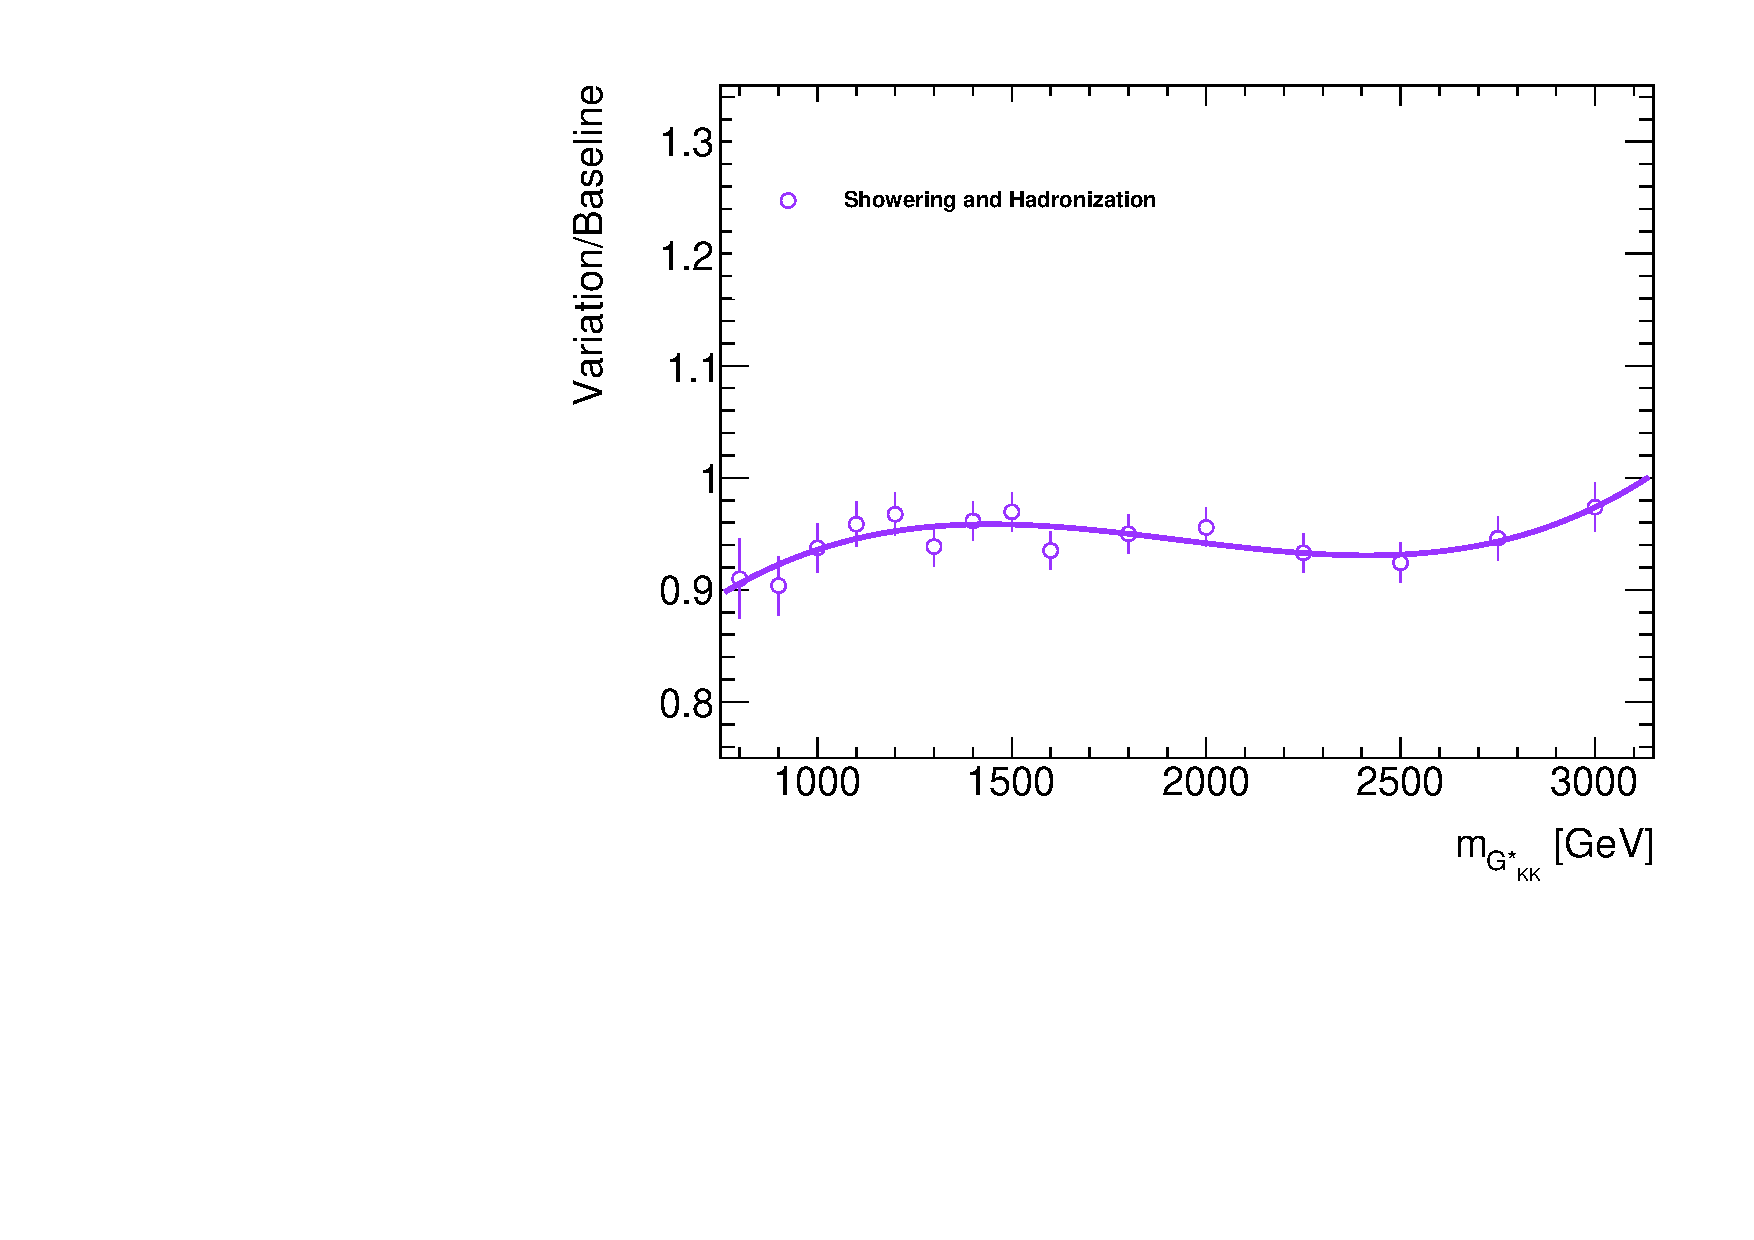
\includegraphics[width=0.3\textwidth, clip]{figures/boosted/Syst_MC/Boosted_3Tag_BulkRSGKKc2_Shower_ratio.pdf}\hspace{5mm}}
% \subfloat[3-Tag: scalar]{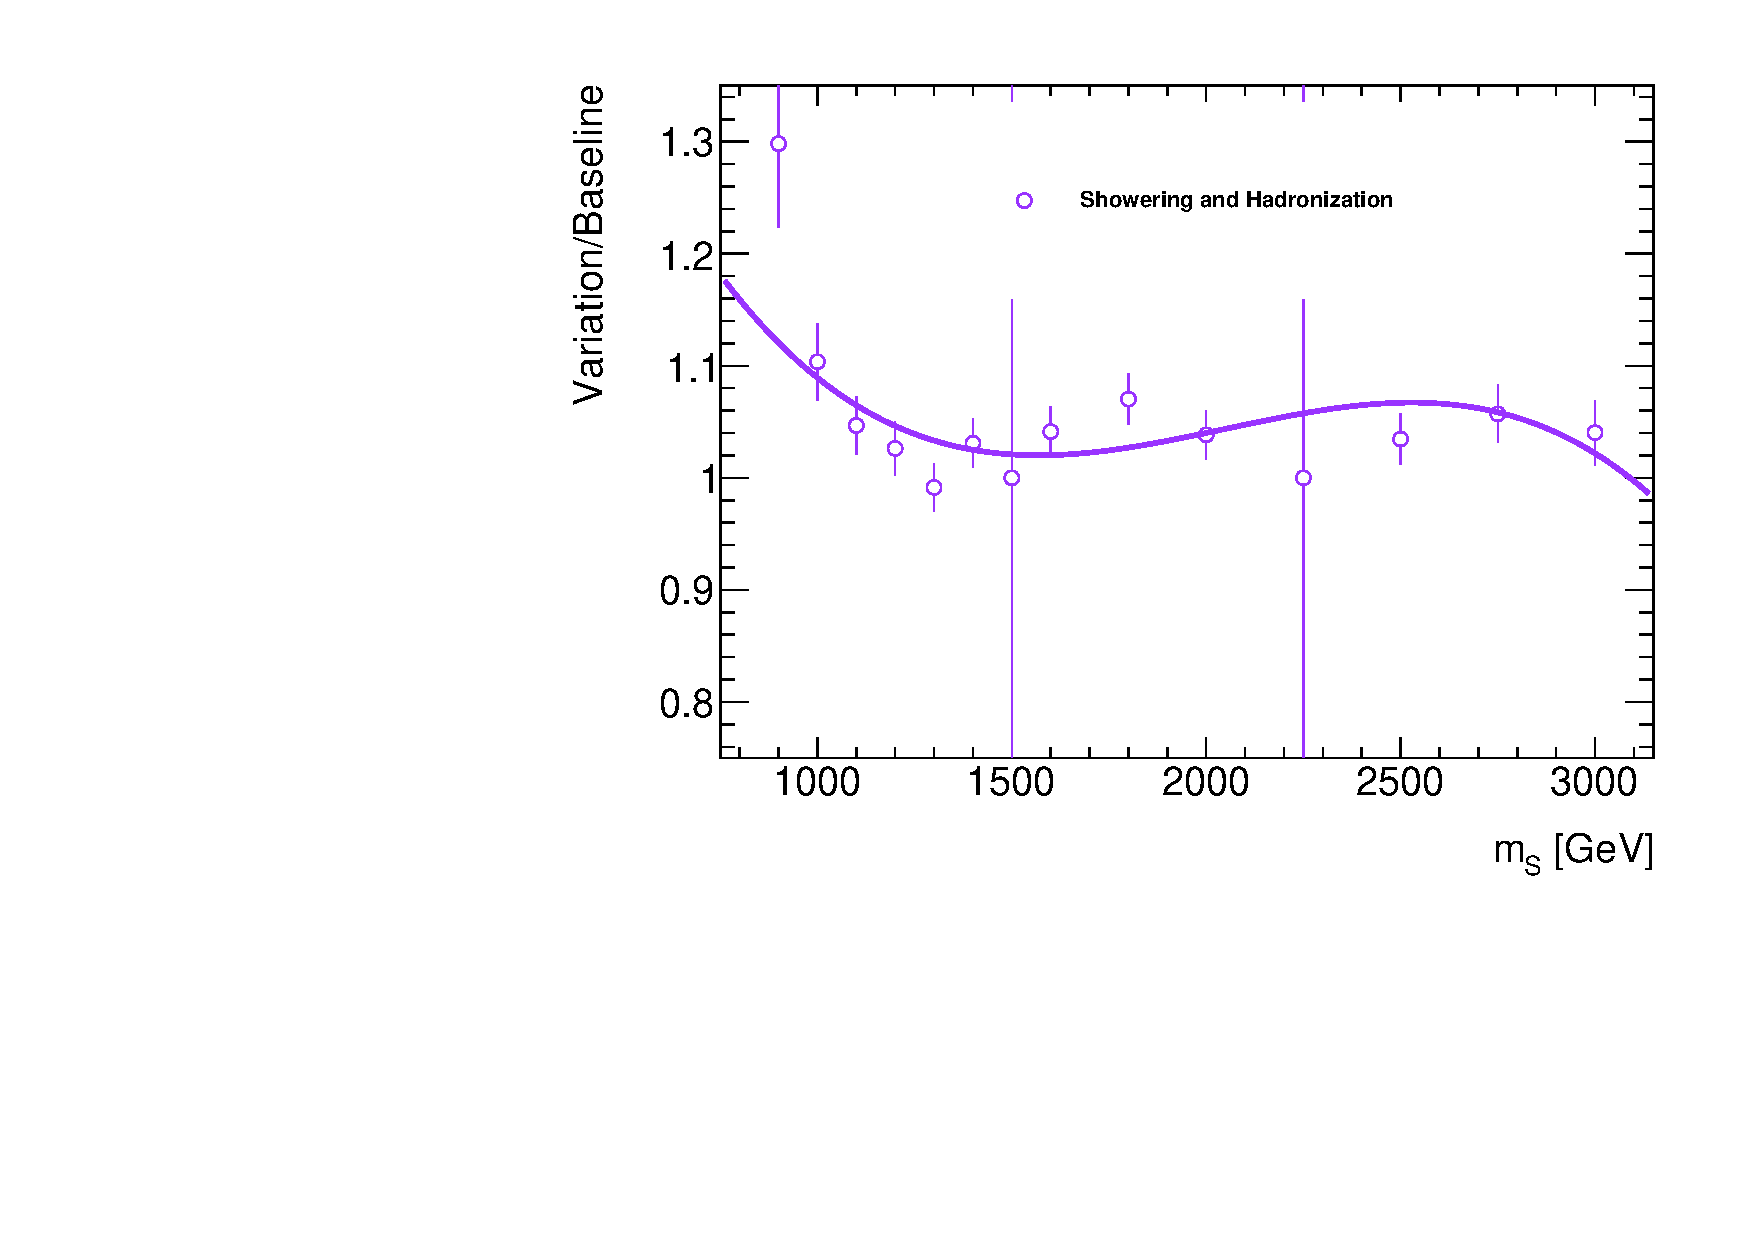
\includegraphics[width=0.3\textwidth, clip]{figures/boosted/Syst_MC/Boosted_3Tag_Scalar_Shower_ratio.pdf}\hspace{5mm}}\\
% \subfloat[4-Tag: bulk RS c=1]{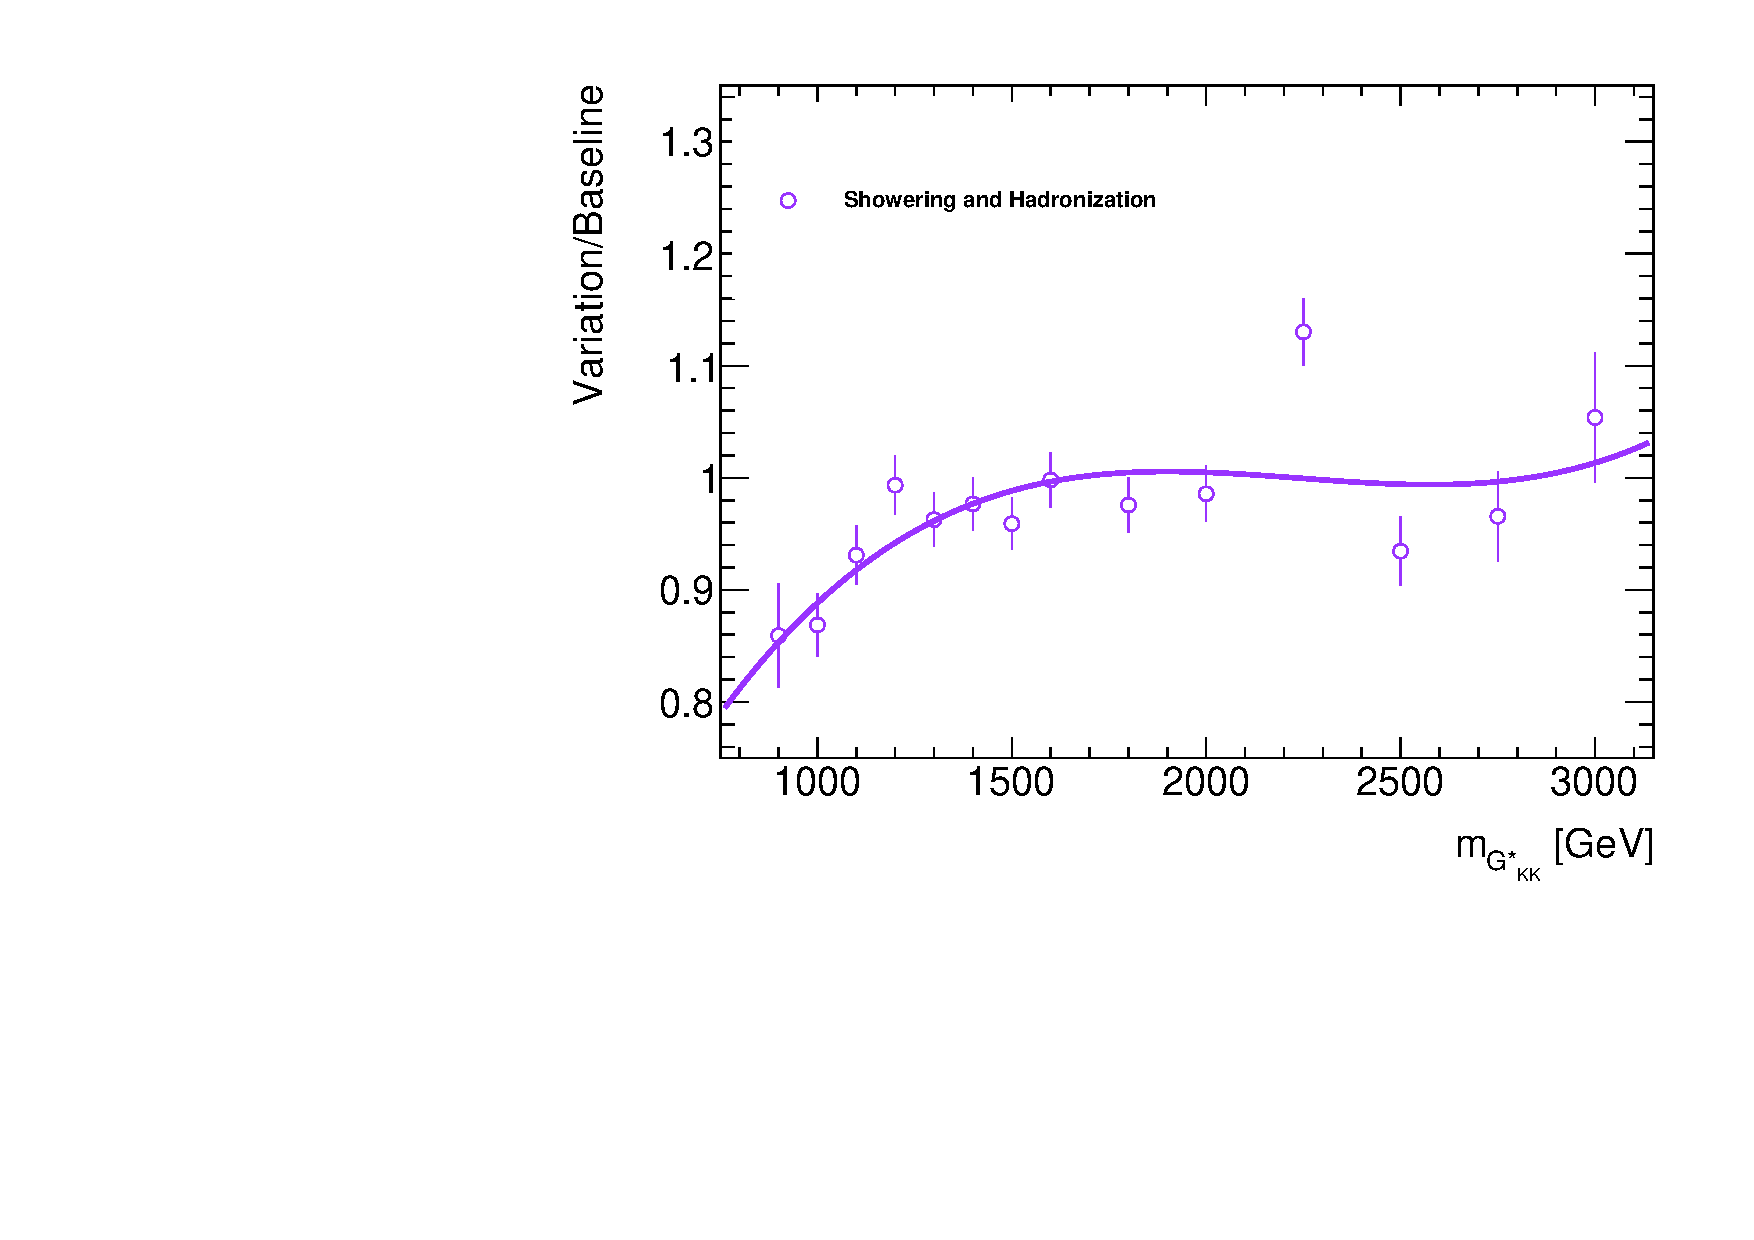
\includegraphics[width=0.3\textwidth, clip]{figures/boosted/Syst_MC/Boosted_4Tag_BulkRSGKKc1_Shower_ratio.pdf}\hspace{5mm}}
% \subfloat[4-Tag: bulk RS c=2]{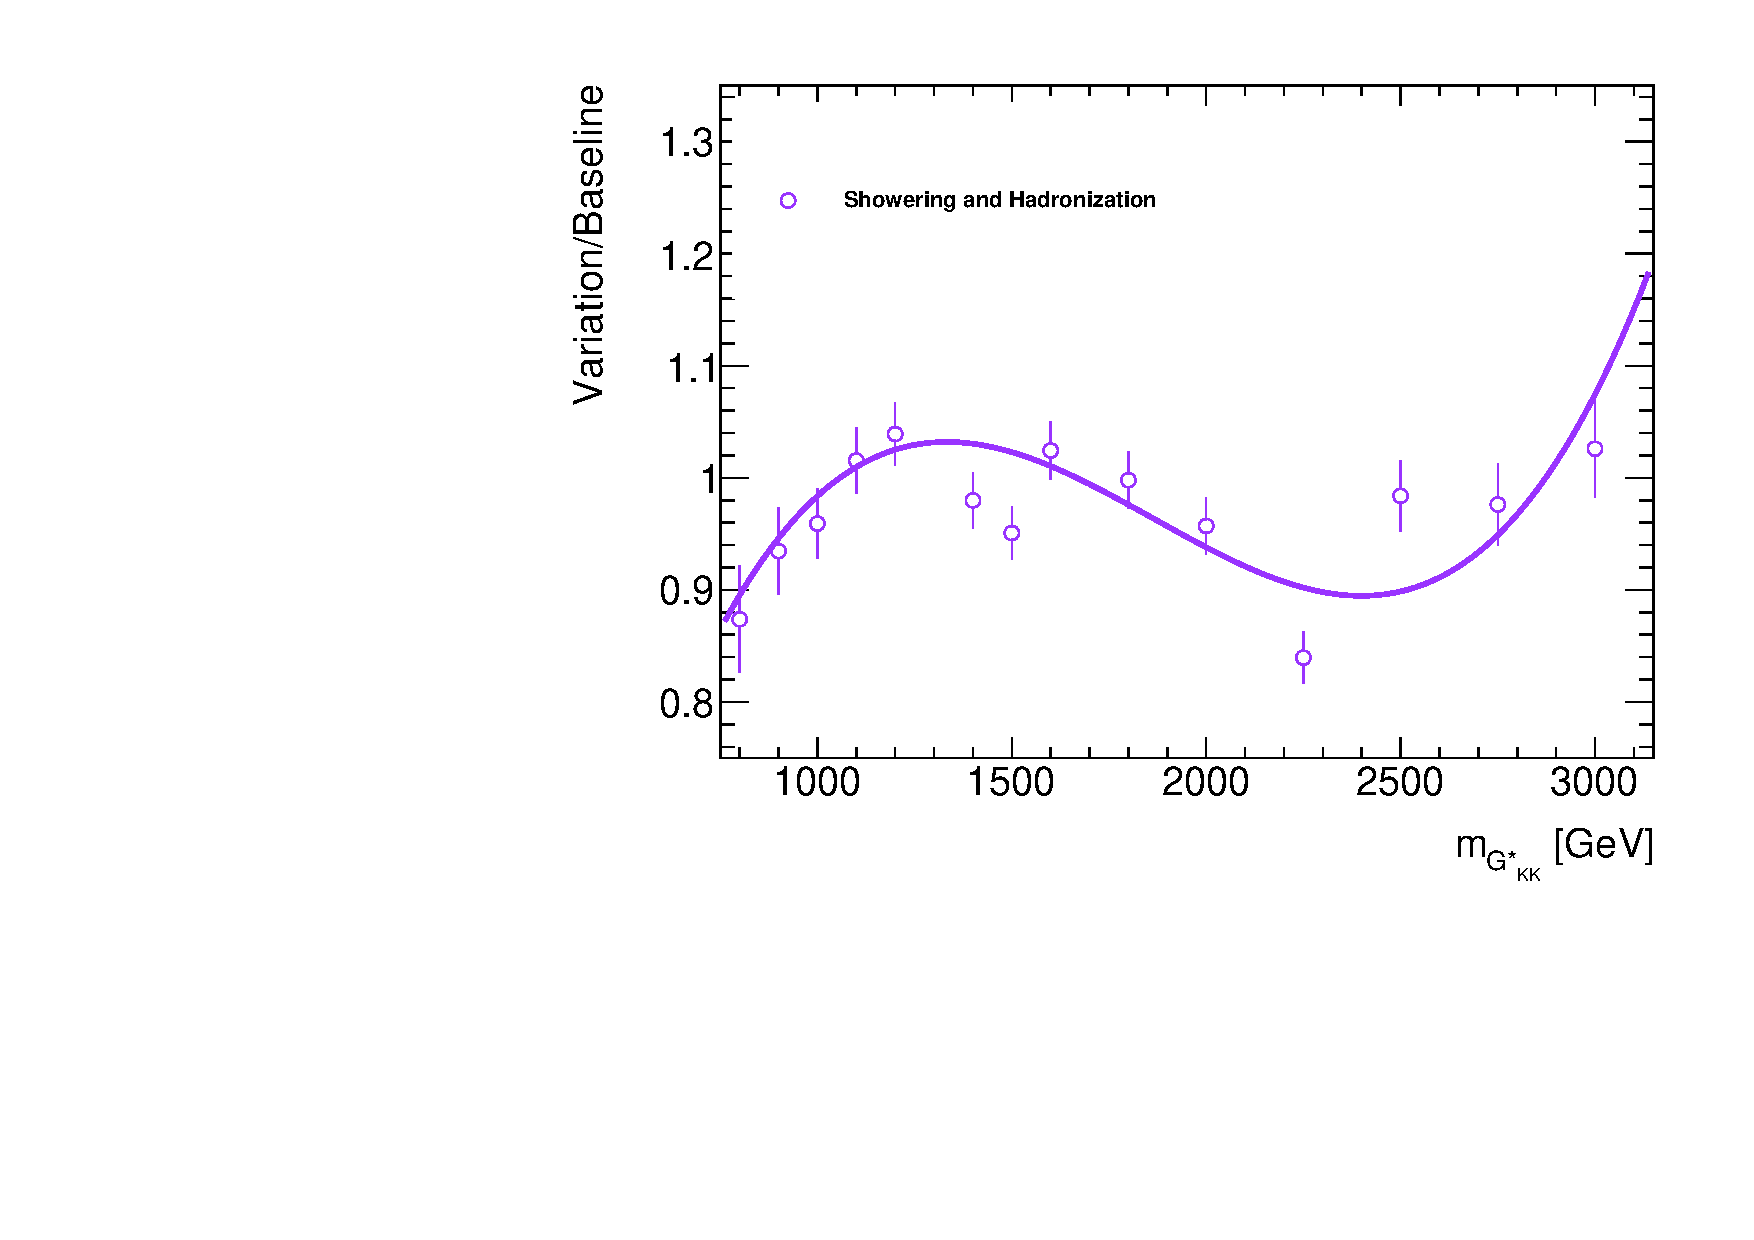
\includegraphics[width=0.3\textwidth, clip]{figures/boosted/Syst_MC/Boosted_4Tag_BulkRSGKKc2_Shower_ratio.pdf}\hspace{5mm}}
% \subfloat[4-Tag: scalar]{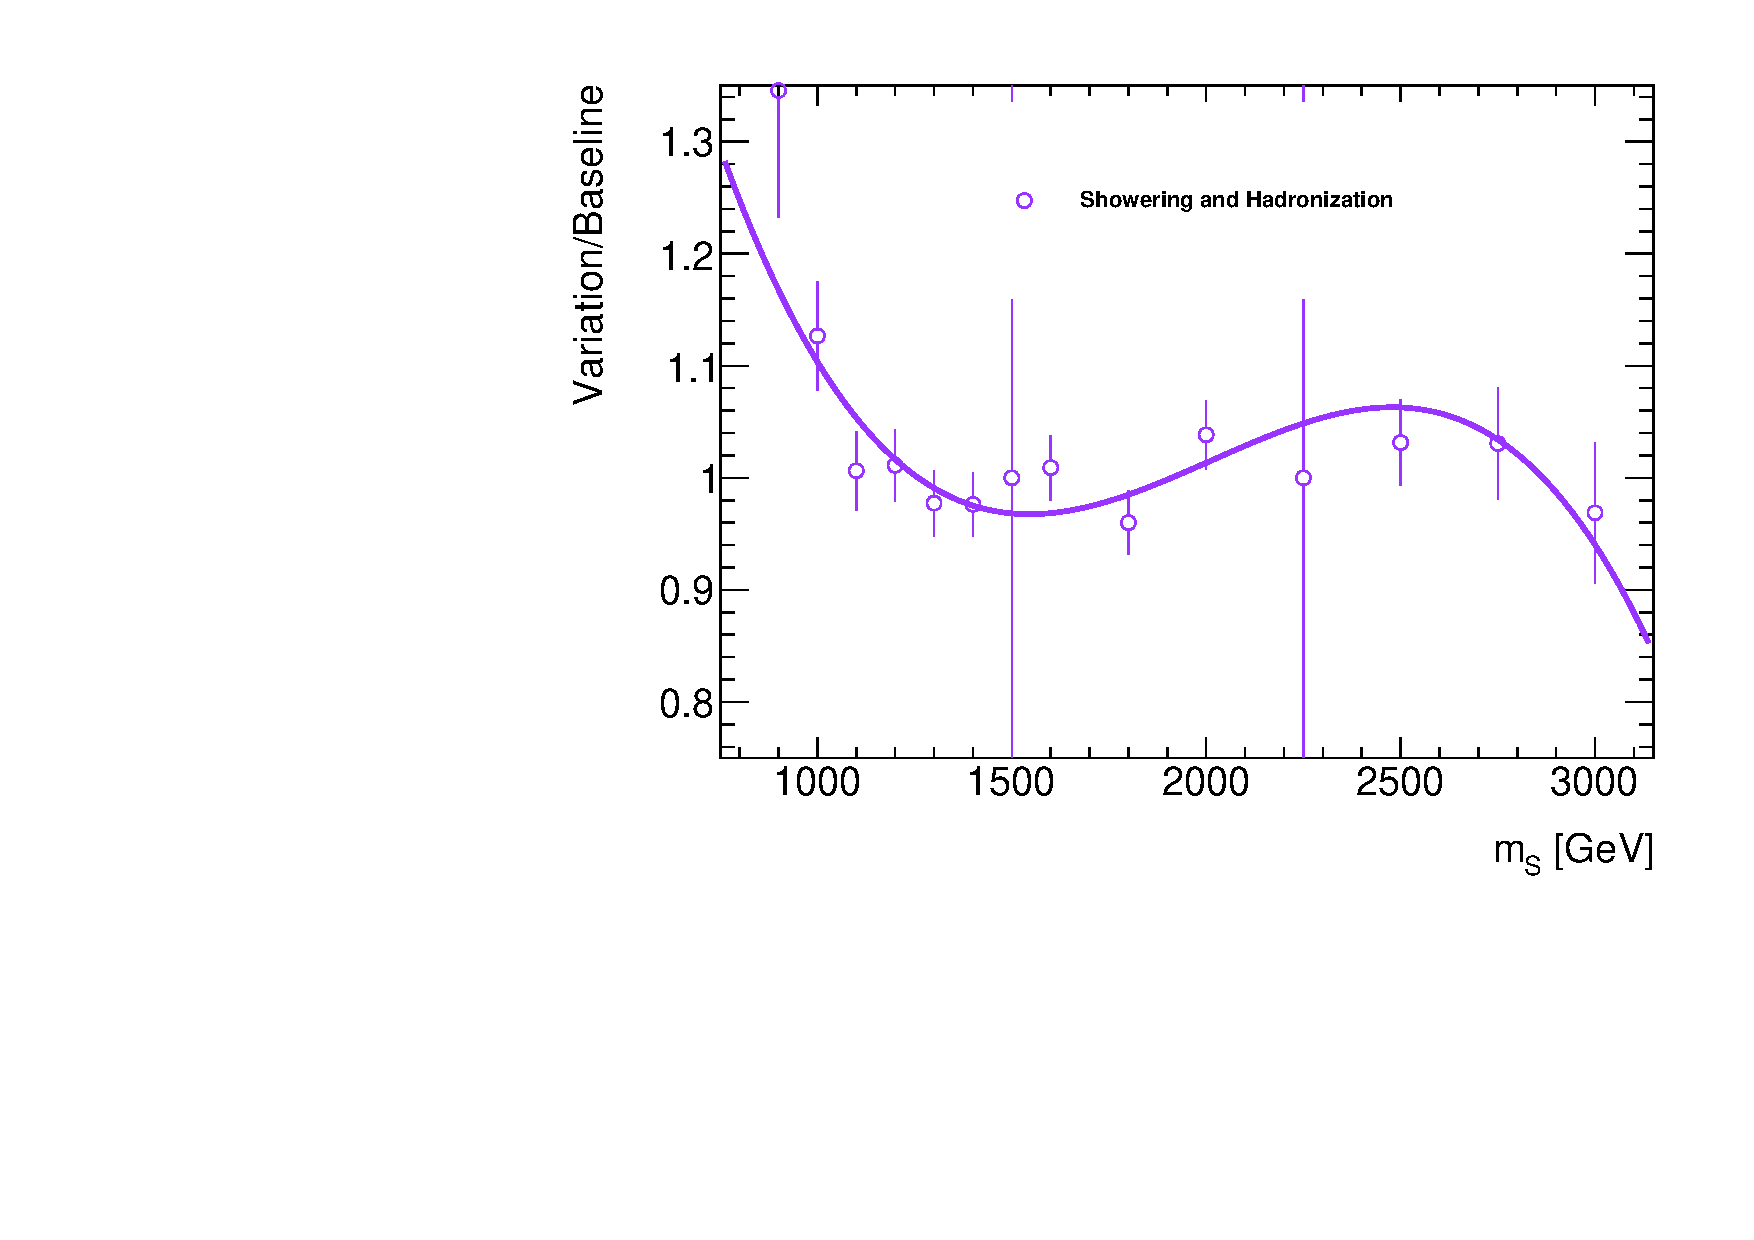
\includegraphics[width=0.3\textwidth, clip]{figures/boosted/Syst_MC/Boosted_4Tag_Scalar_Shower_ratio.pdf}\hspace{5mm}}
% \caption{Ratio of acceptance times efficiency measured in the shower-varied samples over the baseline sample shown as open circles. The polynomial fits shown as solid lines are used to assign the corresponding systematic variation in the final statistical analysis.}
% \label{fig:showerVar}
% \end{center}
% \end{figure*}

%%\paragraph{}
PDF uncertainties are evaluated using the PDF4LHC15\_nlo\_mc set, which combines CT14, MMHT14 and NNPDF3.0 PDF sets \cite{0954-3899-43-2-023001}. The uncertainty is evaluated by calculating the acceptance for each PDF replica. The standard deviation of these acceptance values divided by the baseline acceptance is taken as the PDF uncertainty. For each mass point the distribution of these ratio is compatible with a Gaussian centred on one. The calculated PDF uncertainty is shown in Figure \ref{fig:pdfVar} as upward and downward shifts from unity. The uncertainty in acceptance due to PDF uncertainties is less than $\pm1\%$ across the full mass range considered for the analysis. For this reason, it is neglected in the statistical analysis described in Section \ref{sec:statistical-analysis}.

% \begin{figure*}
% \begin{center}
% \subfloat[2-Tag-Split: bulk RS c=1]{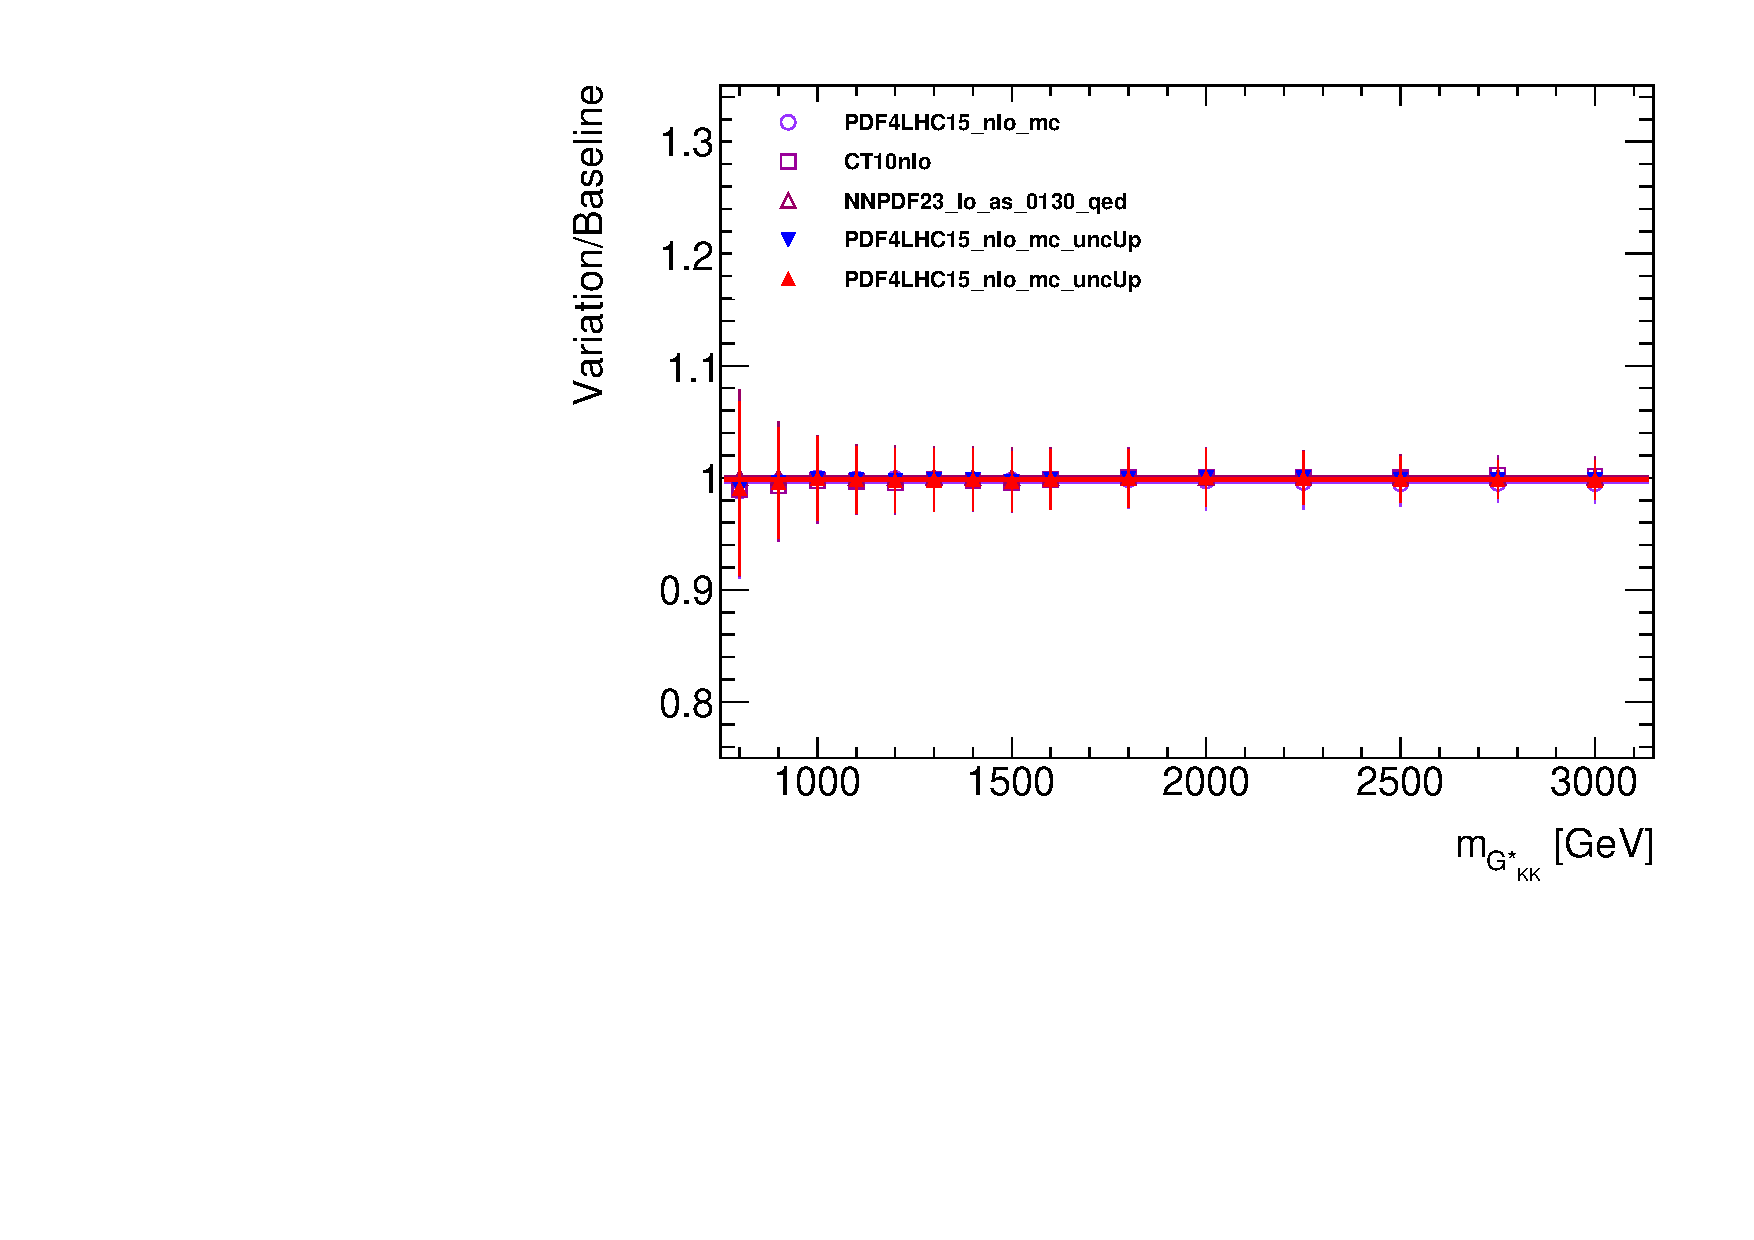
\includegraphics[width=0.3\textwidth, clip]{figures/boosted/Syst_MC/Boosted_2Tag_BulkRSGKKc1_PDF_ratio.pdf}\hspace{5mm}}
% \subfloat[2-Tag-Split: bulk RS c=2]{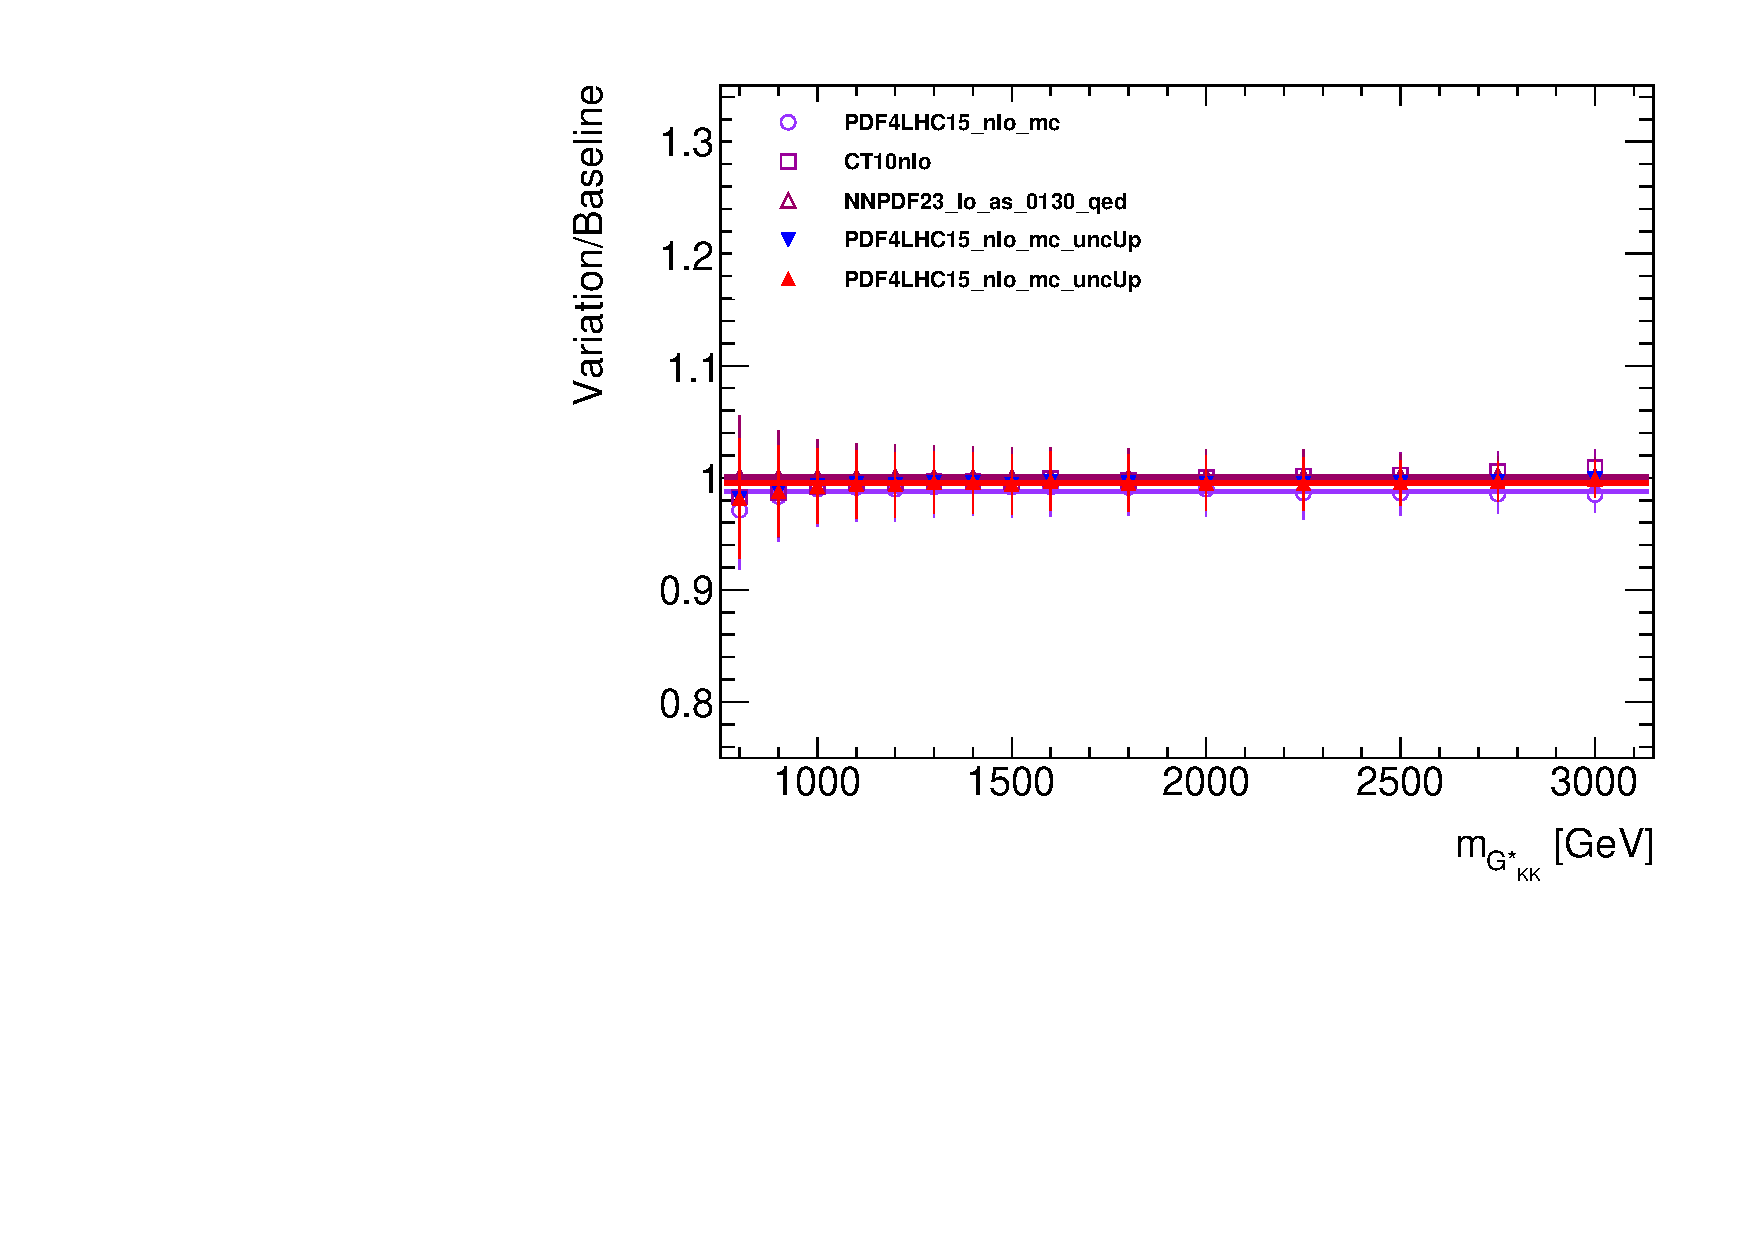
\includegraphics[width=0.3\textwidth, clip]{figures/boosted/Syst_MC/Boosted_2Tag_BulkRSGKKc2_PDF_ratio.pdf}\hspace{5mm}}
% \subfloat[2-Tag-Split: scalar]{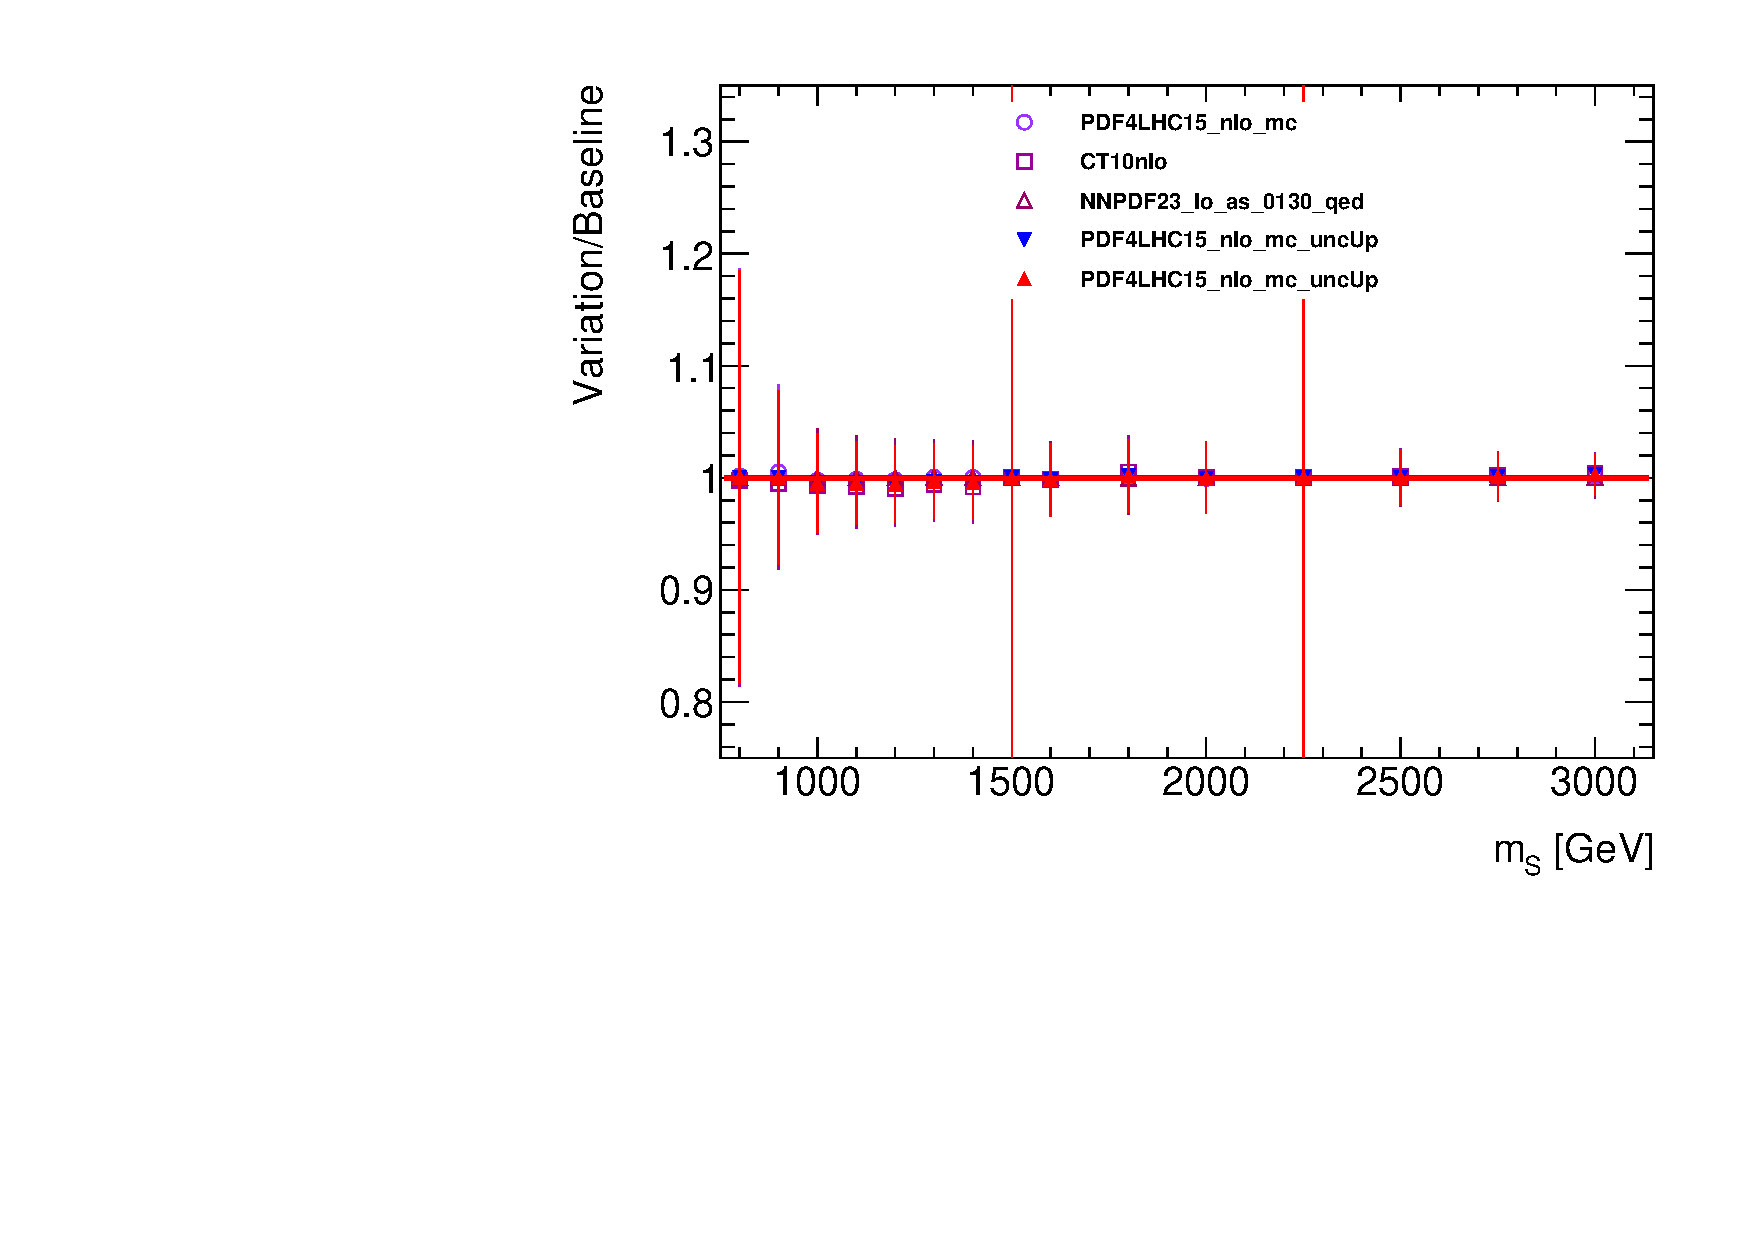
\includegraphics[width=0.3\textwidth, clip]{figures/boosted/Syst_MC/Boosted_2Tag_Scalar_PDF_ratio.pdf}\hspace{5mm}}\\
% \subfloat[3-Tag: bulk RS c=1]{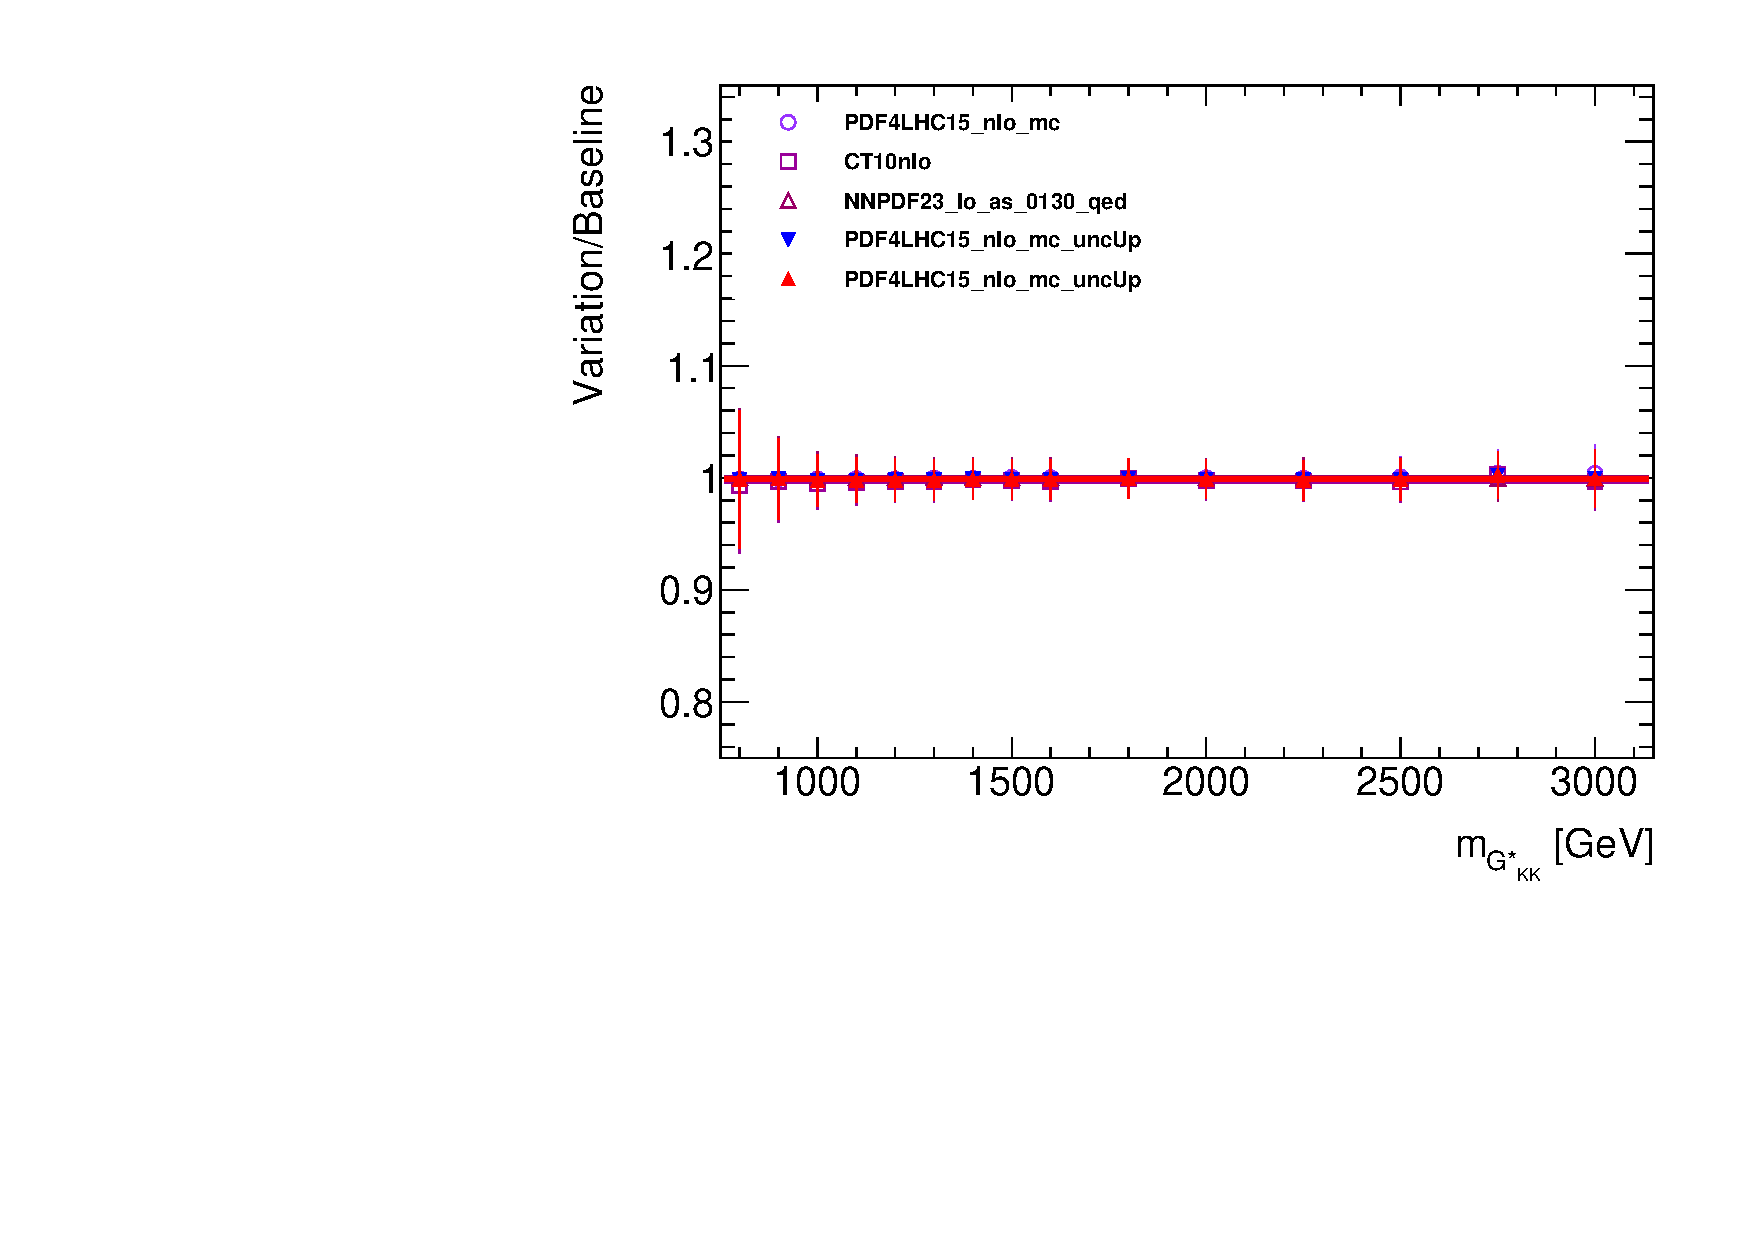
\includegraphics[width=0.3\textwidth, clip]{figures/boosted/Syst_MC/Boosted_3Tag_BulkRSGKKc1_PDF_ratio.pdf}\hspace{5mm}}
% \subfloat[3-Tag: bulk RS c=2]{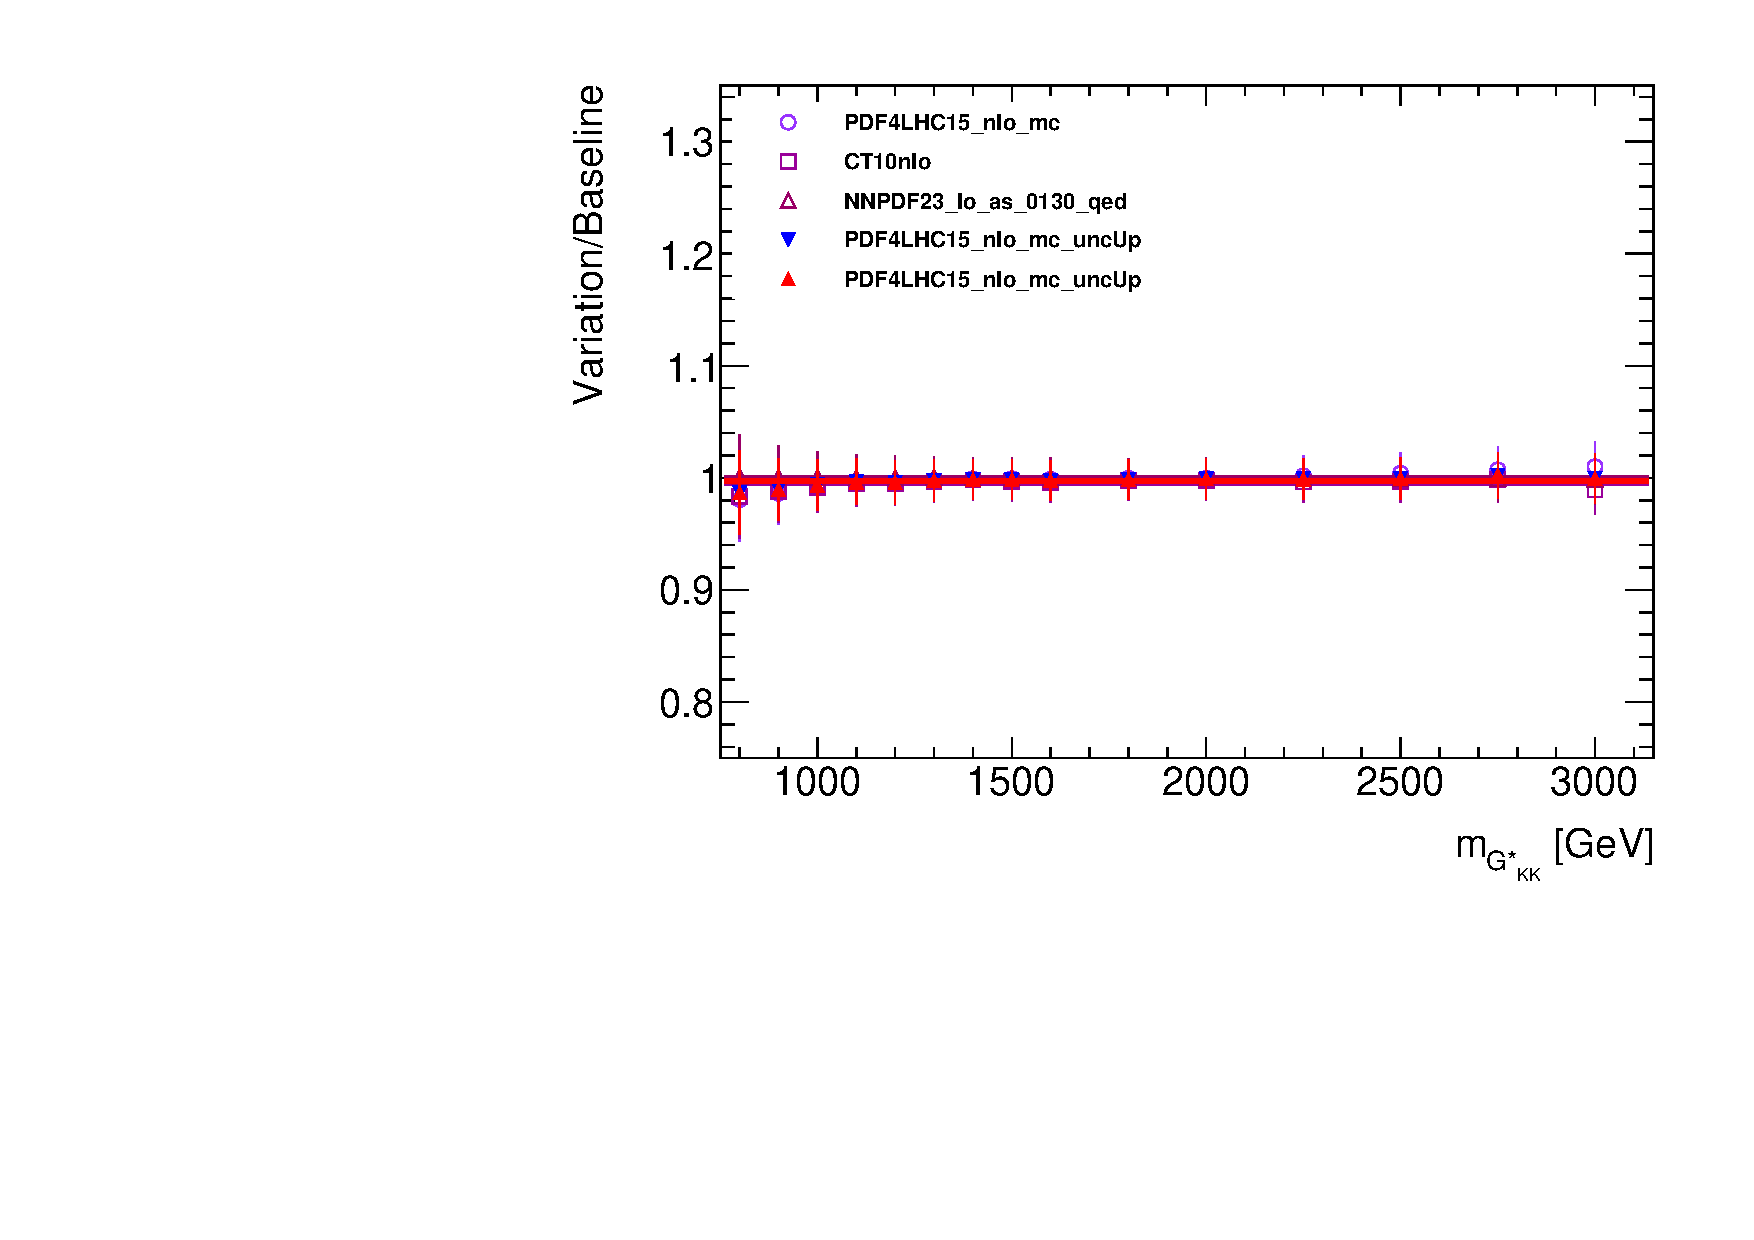
\includegraphics[width=0.3\textwidth, clip]{figures/boosted/Syst_MC/Boosted_3Tag_BulkRSGKKc2_PDF_ratio.pdf}\hspace{5mm}}
% \subfloat[3-Tag: scalar]{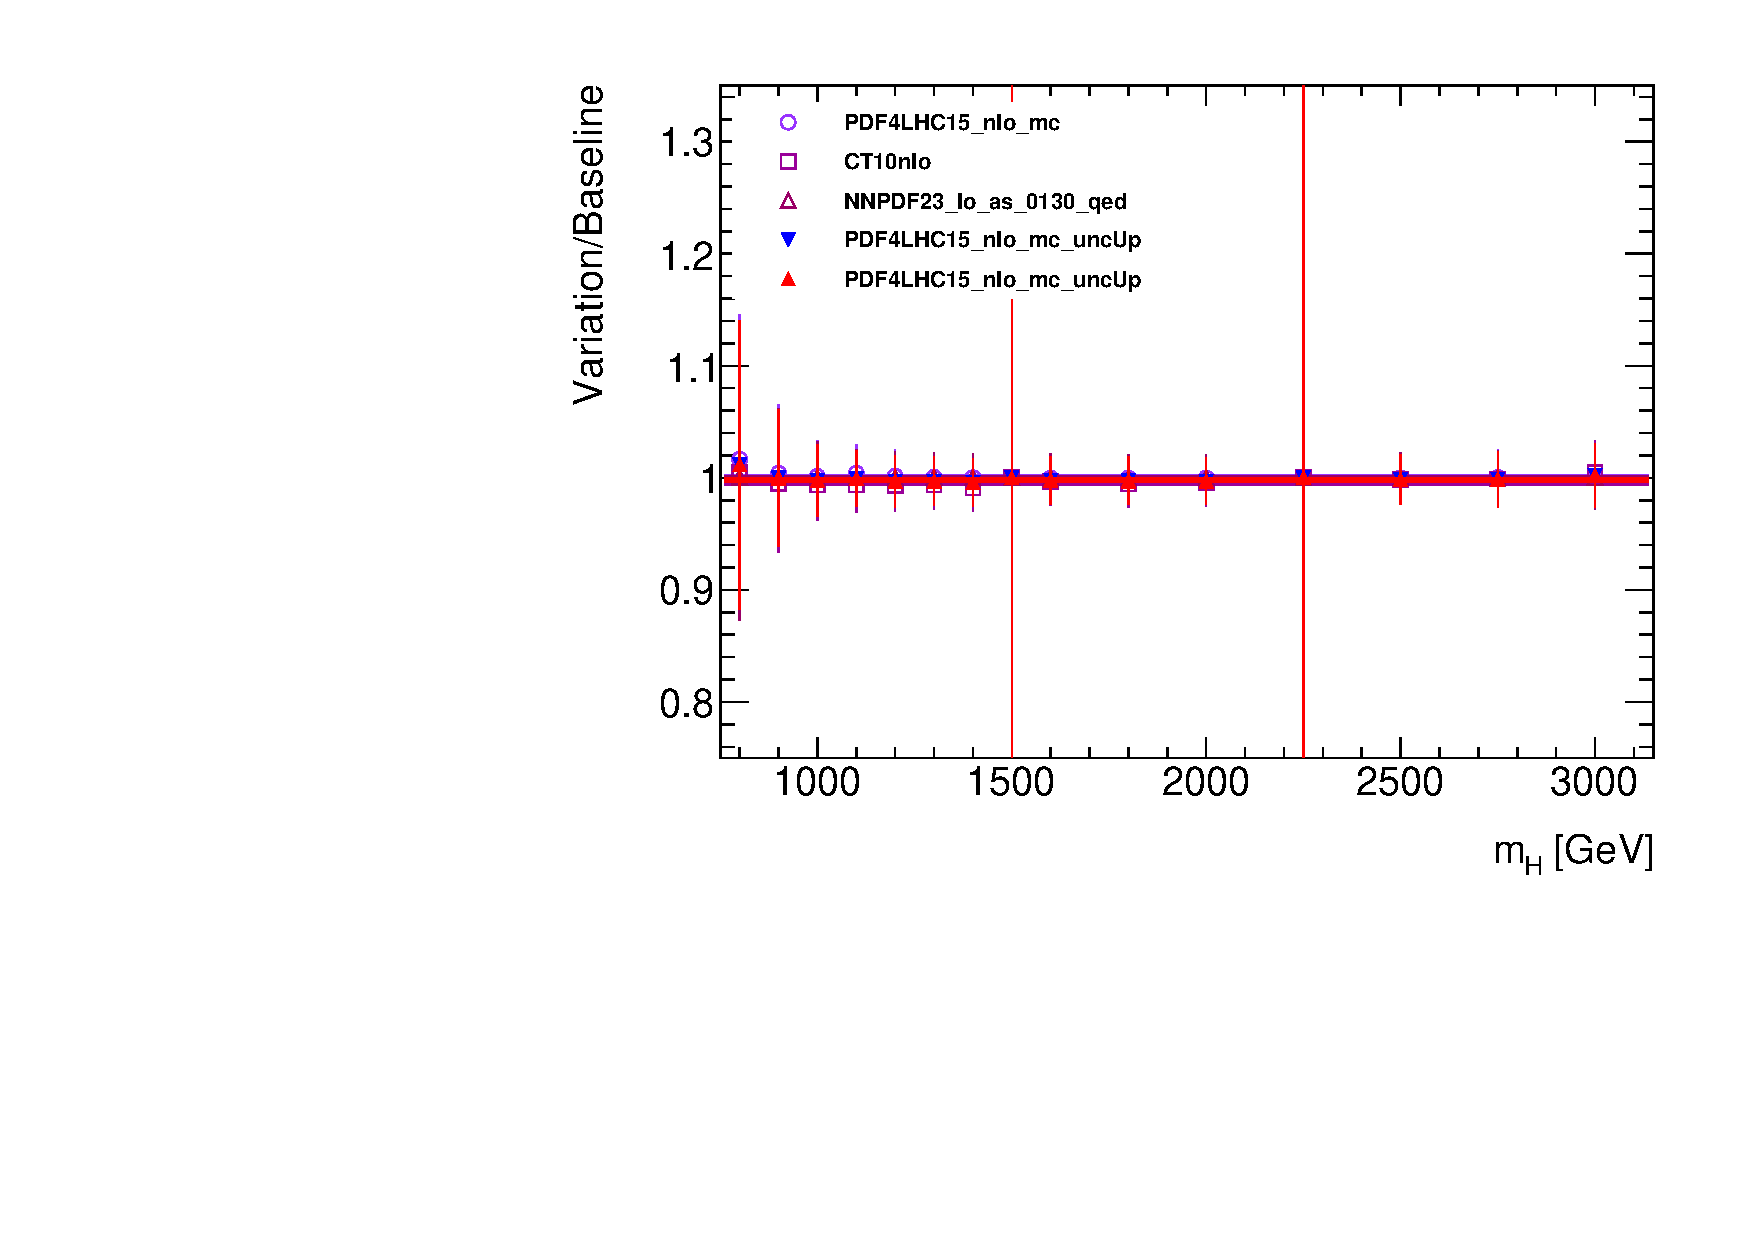
\includegraphics[width=0.3\textwidth, clip]{figures/boosted/Syst_MC/Boosted_3Tag_Scalar_PDF_ratio.pdf}\hspace{5mm}}\\
% \subfloat[4-Tag: bulk RS c=1]{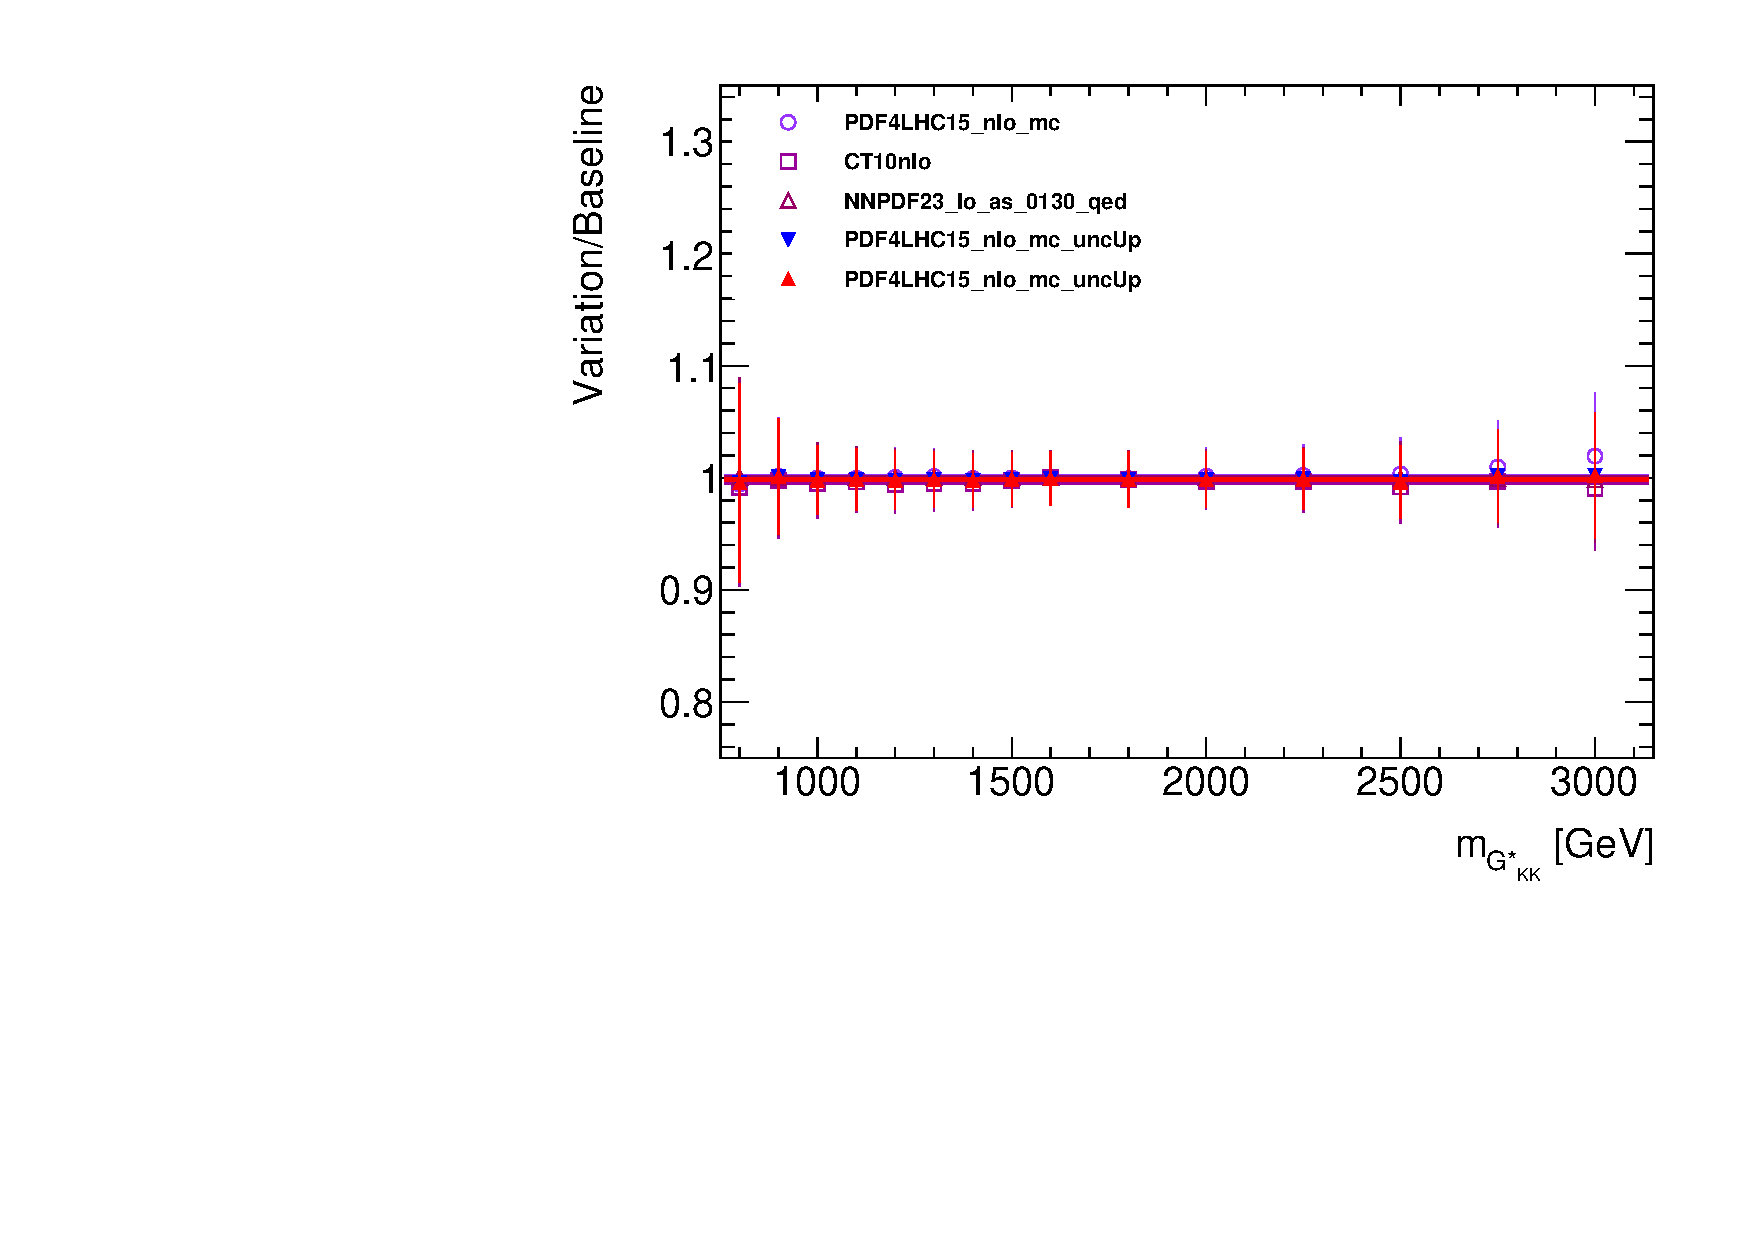
\includegraphics[width=0.3\textwidth, clip]{figures/boosted/Syst_MC/Boosted_4Tag_BulkRSGKKc1_PDF_ratio.pdf}\hspace{5mm}}
% \subfloat[4-Tag: bulk RS c=2]{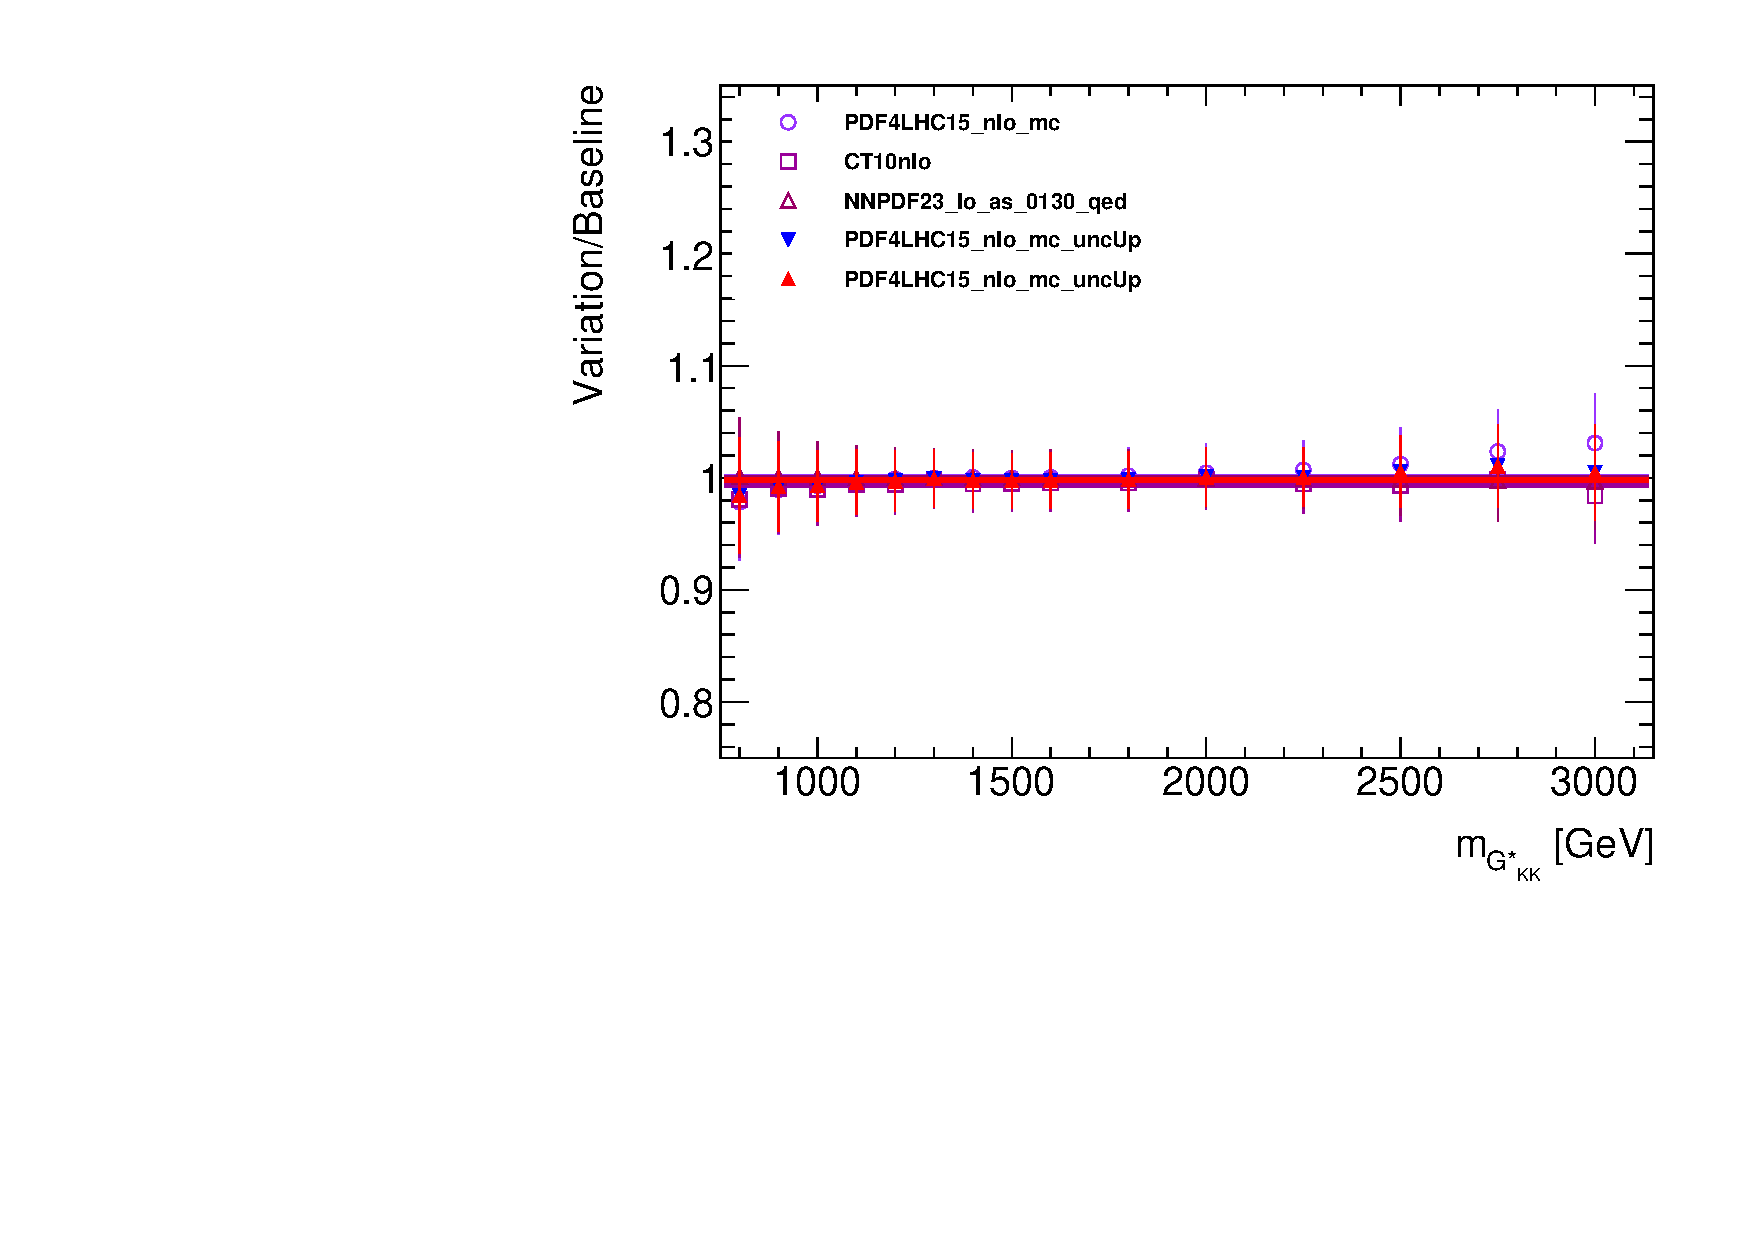
\includegraphics[width=0.3\textwidth, clip]{figures/boosted/Syst_MC/Boosted_4Tag_BulkRSGKKc2_PDF_ratio.pdf}\hspace{5mm}}
% \subfloat[4-Tag: scalar]{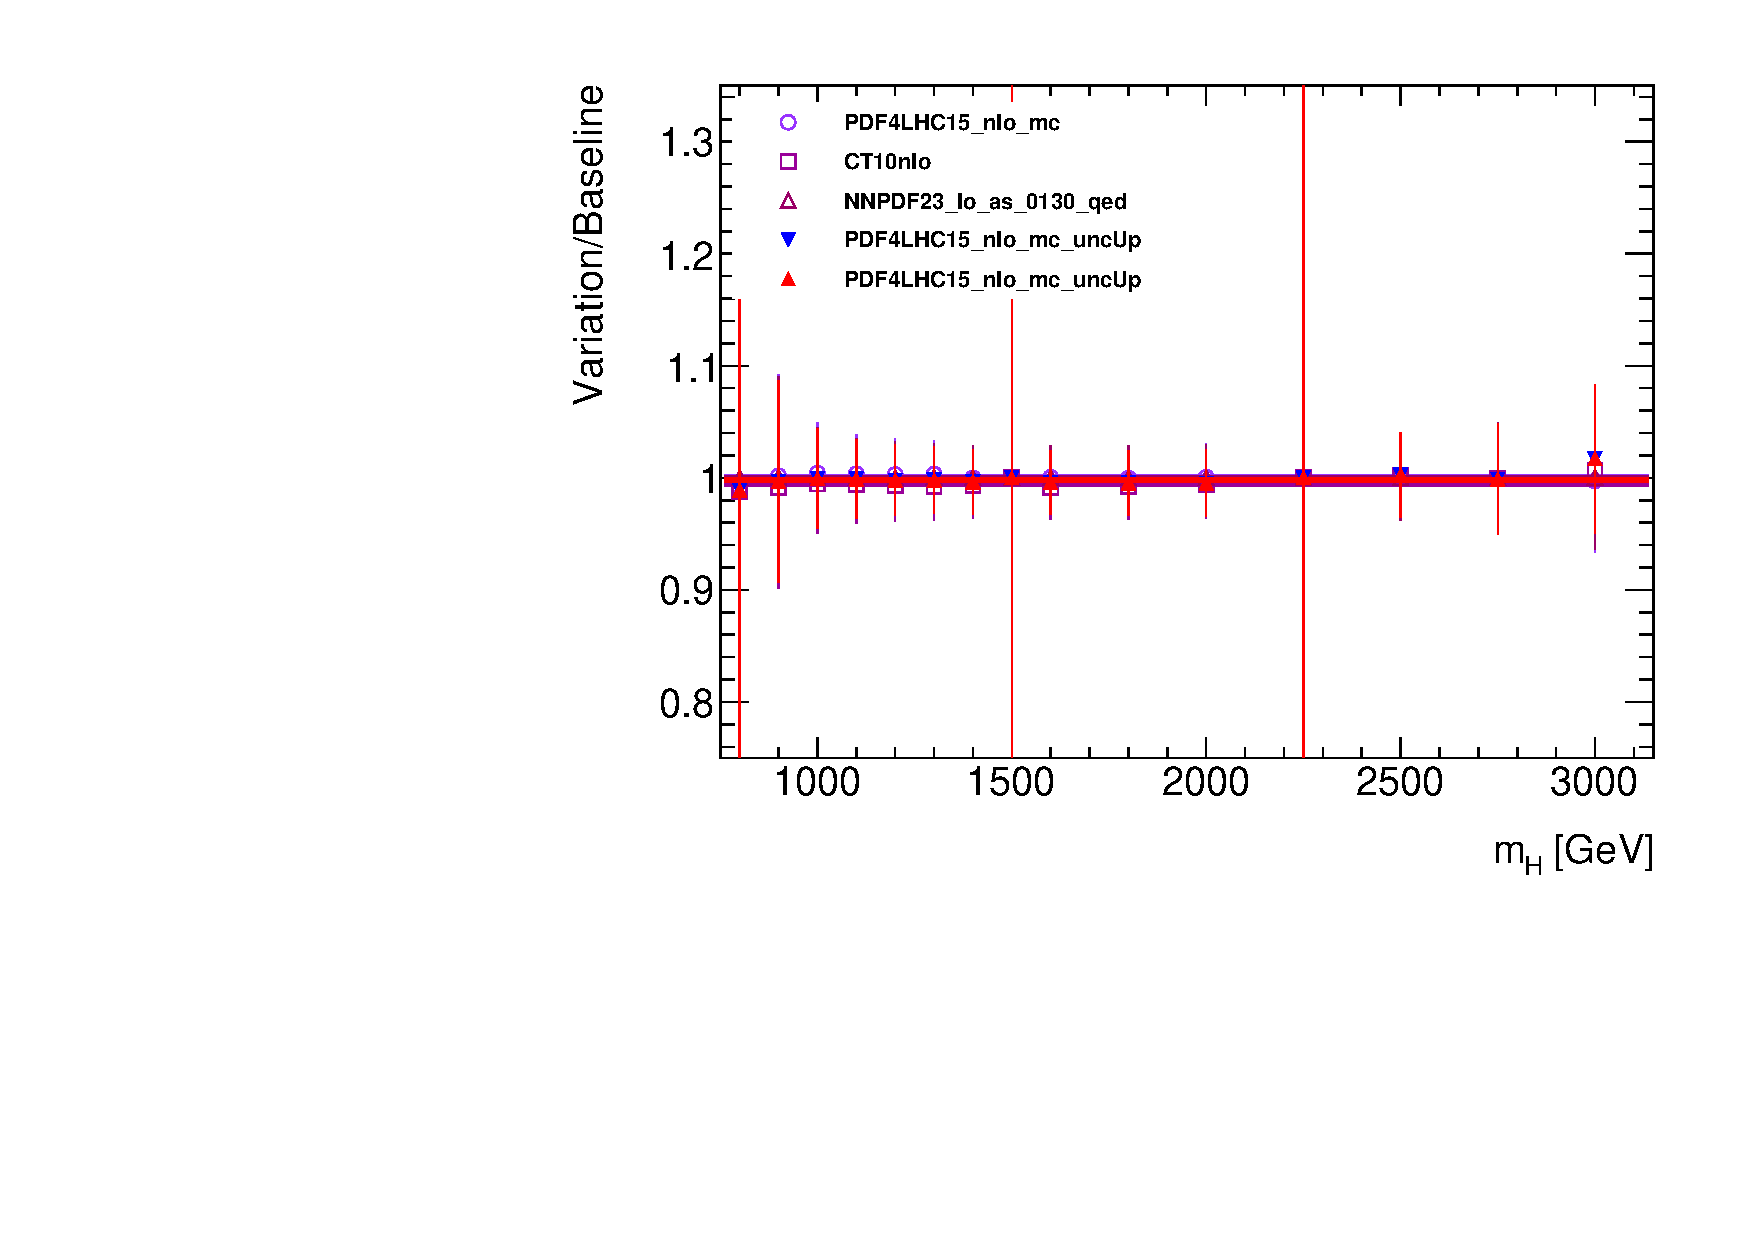
\includegraphics[width=0.3\textwidth, clip]{figures/boosted/Syst_MC/Boosted_4Tag_Scalar_PDF_ratio.pdf}\hspace{5mm}}
% \caption{Ratio of acceptance times efficiency measured in the PDF-varied samples over the baseline sample shown as open circles. Given the consistency with unity, no PDF-uncertainty will be assigned.}
% \label{fig:pdfVar}
% \end{center}
% \end{figure*}

These uncertainties are implemented in the final statistical analysis as normalisation uncertainties on the signals, with the value taken from the polynomial fit. This smooths out statistical fluctuations and allows interpolation between the generated mass points, if needed.

\subsection{Background prediction uncertainty}
\label{sec:boosted-systematics-bkg}
w\paragraph{}
A statistical uncertainty on the value of \muqcd for the $4b$ ($3b$, 2$b$s) Signal Region was determined from the fitting procedure described in Section~\ref{sec:ttbarnorm}. 
%where \muqcd = $0.00084\pm 0.000072$ (stat) in the 4 $b$-tag region, \muqcd = $0.00838 \pm 0.00017$ (stat) in the 3 $b$-tag region, and \muqcd = $0.036 \pm 0.00037$ (stat) in the 2 $b$s-tag region.

\paragraph{}
The statistical uncertainty of the \ttbar\ normalization is accounted for through the uncertainties on \alphatt from the fit to data, as described in Section~\ref{sec:ttbarnorm}. The statistical uncertainty of 69\% on \alphatt are 79\% anti-correlated to the value of \muqcd found in the fitting procedure in the 4 $b$-tag region, the uncertainties of 9\% on \alphatt are 76\% anti-correlated to the value of \muqcd found in the fitting procedure in the 3 $b$-tag region, and the uncertainties of 2.6\% on \alphatt are 75\% anti-correlated to the value of \muqcd found in the fitting procedure in the 2$b$s-tag region.

\paragraph{}
The background systematic uncertainties in the signal region are divided into the following components:
\begin{itemize}
 \item Non-closure uncertainty on \muqcd found by comparing the value derived from the sideband to the control region normalization.
 \item Effects on the QCD prediction from variations of the SideBand and Control Region Definitions
 \item The impact of the shape uncertainty of the \ttbar\ distribution in the $4b$ signal region.
 \item The impact of the shape uncertainty of the 1/2$b$ QCD distribution derived in the control region.
 \item The impact of the smoothing function fit range and function choice on the QCD prediction
\end{itemize}

\paragraph{}
The \ttbar\ normalization uncertainty on \alphatt is derived in the fit to data as described in Section~\ref{sec:ttbarnorm}. This has a negligible impact on the signal sensitivity, but is still propagated as the uncertainty in the \ttbar\ normalization in the signal region.

%However, the \ttbar\ background estimation can impact the value of $\mu_{QCD}$ used to determine the QCD normalization in the signal region, where a 53\% (60\%) correlation was found in the fitting procedure between \muqcd and \alphatt in the 4 (3) $b$-tag region This and the other background uncertainty components will be discussed in this section. 

\subsubsection{Non-closure uncertainty on \muqcd determined in the control region}
\label{sec:non-closure-mu-qcd}

\paragraph{}
A further uncertainty is derived by comparing the value of \muqcd to the overall difference between predicted to observed events in the control region. While the total predicted background (showing stat error only) of 4$b$: 76.7 $\pm$ 5.4 vs obs 81.0, 3$b$: 1565.6 $\pm$ 18.1 vs obs 1553.0, 2$b$s: 8332.4 $\pm$ 38.8 vs obs 8486.0, the number events agrees with the total data in the control region within statistical error, we consider an added systematic on the background prediction normalization, taken a as the maximum between either the difference between the central value of the prediction to the observed number of events (4.3 events, or 5\%, for 4$b$.  13 events, or 1\%, for 3$b$; 154 events, or 2\%, for 2$b$s) or the statistical uncertainty of the observed 4b (3b) data in the CR (11.1\% for $4b$; 2.5\% for $3b$; and 1.1\% for 2$b$s). For the detailed numbers, please refer to section ~\ref{sec:yields}. 

\paragraph{}
Although we have derived our non-closure uncertainty on $\mu_{QCD}$ from comparison between data and prediction in the control region, we need to test how this number is sensitive to our choice of control region (CR) and sideband region (SB). In addition, we also want to check how our background prediction in signal region is sensitive to the choice of control region and sideband region. All these tests are done on the control/sideband regions after the full reweighting procedure as described in \ref{sec:boosted-reweight}, while applying the nominal reweighting values.

\paragraph{}
Besides the nominal control region as described above, we design three additional control regions, as illustrated in Figure \ref{CRSB:CR_High}, \ref{CRSB:CR_Low}, \ref{CRSB:CR_Small}, \ref{CRSB:SB_High}, \ref{CRSB:SB_Low}, \ref{CRSB:SB_Large}, \ref{CRSB:SB_Small}:
\begin{itemize}
	\item Low-mass CR: the center position of the circle that defines nominal CR is moved down by 3 GeV, in both leading and sub-leading large-jet mass.
	\item High-mass CR: the center position of the circle that defines nominal CR is moved up by 3 GeV, in both leading and sub-leading large-R jet mass.
	\item Signal-depletion (Small) CR: the $X_{hh}$ cut that defines signal region is increased to $2.0$ from $1.6$. This variation only affect CR, while SR remains unchanged (i.e. signal region is still defined by $X_{hh}<1.6$, while CR is defined as $X_{hh}>2.0$ and $R_{hh}<33$).
	\item High-mass SB: The signal region and control region remain unchanged, the center position of the circle that defines nominal SB is moved up by 3 GeV in both leading and sub-leading large-R jet mass.
	\item Low-mass SB: The signal region and control region remain unchanged, the center position of the circle that defines nominal SB is moved up by 3 GeV in both leading and sub-leading large-R jet mass.
	\item Large SB: The signal region and control region remain unchanged, while the SB is $33 < R_{hh}$ and $ R_{hh}^{\text{high}} < 61$. $\mu_{QCD}$ will change.
	\item Small SB: The signal region and control region remain unchanged, while the SB is $33 < R_{hh}$ and $ R_{hh}^{\text{high}} < 55$. $\mu_{QCD}$ will change.
\end{itemize}

\paragraph{}
%To ensure that these value cover the QCD normalization uncertainty, further checks on the effect of adjusting the Control and Sideband definitions were done. 
The results are summarized in Table \ref{CRSB:Tab_4b_CR_Variations}, \ref{CRSB:Tab_3b_CR_Variations} and \ref{CRSB:Tab_2bs_CR_Variations}, while the details are presented in the Appendix~\ref{app:boosted-syst-CRSB_Definition_Variation}. Based on all the variations, a 2.8\% normalization uncertainty is assigned to 2$b$s region, 4.2\% to 3$b$ region (which is the statistical uncertainty), and a 12.2\% normalization uncertainty is assigned to 4$b$ region.

\begin{table}[htbp!]
\begin{center}
\begin{footnotesize} 
\begin{tabular}{c|c|c|c} 
CR Varations FourTag & Data & Prediction & (Predict - Data)/Data \\ 
\hline\hline 
& & & \\ 
Nominal & 81.0 $\pm$ 9.0 & 76.77 $\pm$ 5.43 & -5.22 $\%$  $\pm$ 17.23 $\%$ \\ 
\hline 
CR High & 76.0 $\pm$ 8.72 & 71.12 $\pm$ 5.41 & -6.43 $\%$  $\pm$ 17.85 $\%$ \\ 
\hline 
CR Low & 91.0 $\pm$ 9.54 & 79.87 $\pm$ 5.45 & -12.2 $\%$  $\pm$ 15.19 $\%$ \\ 
\hline 
CR Small & 58.0 $\pm$ 7.62 & 55.96 $\pm$ 5.35 & -3.52 $\%$  $\pm$ 21.89 $\%$ \\ 
\hline 
SB Large & 81.0 $\pm$ 9.0 & 74.71 $\pm$ 5.4 & -7.76 $\%$  $\pm$ 16.91 $\%$ \\ 
\hline 
SB Small & 81.0 $\pm$ 9.0 & 74.15 $\pm$ 5.38 & -8.45 $\%$  $\pm$ 16.81 $\%$ \\ 
\hline 
SB High & 81.0 $\pm$ 9.0 & 78.72 $\pm$ 5.46 & -2.82 $\%$  $\pm$ 17.54 $\%$ \\ 
\hline 
SB Low & 81.0 $\pm$ 9.0 & 76.51 $\pm$ 5.38 & -5.54 $\%$  $\pm$ 17.14 $\%$ \\ 
& & & \\ 
\hline\hline 
\end{tabular} 
\end{footnotesize} 
\newline 

\end{center}
\caption{Agreement between data and prediction in 4b tag CR. Showing stat uncertainty only.}
\label{CRSB:Tab_4b_CR_Variations}
\end{table}

\begin{table}[htbp!]
\begin{center}
\begin{footnotesize} 
\begin{tabular}{c|c|c|c} 
CR Varations ThreeTag & Data & Prediction & (Predict - Data)/Data \\ 
\hline\hline 
Nominal & 1553.0 $\pm$ 39.41 & 1587.04 $\pm$ 21.4 & 2.19 $\%$  $\pm$ 3.97 $\%$ \\ 
\hline 
CR High & 1461.0 $\pm$ 38.22 & 1473.89 $\pm$ 20.77 & 0.88 $\%$  $\pm$ 4.06 $\%$ \\ 
\hline 
CR Low & 1628.0 $\pm$ 40.35 & 1697.38 $\pm$ 21.75 & 4.26 $\%$  $\pm$ 3.92 $\%$ \\ 
\hline 
CR Small & 1134.0 $\pm$ 33.67 & 1127.34 $\pm$ 17.66 & -0.59 $\%$  $\pm$ 4.51 $\%$ \\ 
\hline 
SB Large & 1553.0 $\pm$ 39.41 & 1574.23 $\pm$ 21.47 & 1.37 $\%$  $\pm$ 3.95 $\%$ \\ 
\hline 
SB Small & 1553.0 $\pm$ 39.41 & 1601.44 $\pm$ 21.64 & 3.12 $\%$  $\pm$ 4.01 $\%$ \\ 
\hline 
SB High & 1553.0 $\pm$ 39.41 & 1602.74 $\pm$ 21.48 & 3.2 $\%$  $\pm$ 4.0 $\%$ \\ 
\hline 
SB Low & 1553.0 $\pm$ 39.41 & 1576.56 $\pm$ 21.5 & 1.52 $\%$  $\pm$ 3.96 $\%$ \\ 
\hline\hline 
\end{tabular} 
\end{footnotesize} 
\newline 

\end{center}
\caption{Agreement between data and prediction in 3b tag CR. Showing stat uncertainty only.}
\label{CRSB:Tab_3b_CR_Variations}
\end{table}
\begin{table}[htbp!]
\begin{center}
\begin{footnotesize} 
\begin{tabular}{c|c|c|c} 
CR Varations TwoTag split & Data & Prediction & (Predict - Data)/Data \\ 
\hline\hline 
& & & \\ 
Nominal & 8486.0 $\pm$ 92.12 & 8332.97 $\pm$ 38.84 & -1.8 $\%$  $\pm$ 1.52 $\%$ \\ 
\hline 
CR High & 8174.0 $\pm$ 90.41 & 7937.59 $\pm$ 39.61 & -2.89 $\%$  $\pm$ 1.56 $\%$ \\ 
\hline 
CR Low & 8907.0 $\pm$ 94.38 & 8800.86 $\pm$ 39.51 & -1.19 $\%$  $\pm$ 1.49 $\%$ \\ 
\hline 
CR Small & 5999.0 $\pm$ 77.45 & 5873.52 $\pm$ 32.31 & -2.09 $\%$  $\pm$ 1.8 $\%$ \\ 
\hline 
SB Large & 8486.0 $\pm$ 92.12 & 8341.7 $\pm$ 38.44 & -1.7 $\%$  $\pm$ 1.52 $\%$ \\ 
\hline 
SB Small & 8486.0 $\pm$ 92.12 & 8333.25 $\pm$ 39.12 & -1.8 $\%$  $\pm$ 1.53 $\%$ \\ 
\hline 
SB High & 8486.0 $\pm$ 92.12 & 8378.14 $\pm$ 38.45 & -1.27 $\%$  $\pm$ 1.52 $\%$ \\ 
\hline 
SB Low & 8486.0 $\pm$ 92.12 & 8356.86 $\pm$ 39.06 & -1.52 $\%$  $\pm$ 1.53 $\%$ \\ 
& & & \\ 
\hline\hline 
\end{tabular} 
\end{footnotesize} 
\newline 

\end{center}
\caption{Agreement between data and prediction in 2bs tag CR. Showing stat uncertainty only.}
\label{CRSB:Tab_2bs_CR_Variations}
\end{table}





%\clearpage
%\subsubsection{Effects on QCD normalization prediction from variations of the Sideband and Control Region Definitions}
%\label{sec:boosted-CR-SB-Definition-Variation}
%\input{Sections/sec-systematics-CRSB_Definition_Variation}

\clearpage
\subsubsection{Validation of background estimation from low mass and high mass signal region}
\label{sec:boosted-ZZ-Rehearsal}
%%\paragraph{}
Another check is the the so-called "low mass signal region rehearsal" (or ZZ region) and "high mass signal region rehearsal" (or TT region). Instead of a signal region around di-Higgs mass region on leading-subleading large-R jet mass 2D plane, we redefine a separate lower mass (ZZ) and higher mass (TT) signal region: 
\begin{equation}
X_{ZZ} = \sqrt{\left(\frac{m(J_1) - \text{103 GeV}}{0.1 m(J_1)}\right)^2 + \left(\frac{m(J_2) - \text{96 GeV}}{0.1 m(J_2)}\right)^2} < 1.6 
\label{eq:boosted_Xzz}
\end{equation}
\begin{equation}
X_{TT} = \sqrt{\left(\frac{m(J_1) - \text{164 GeV}}{0.1 m(J_1)}\right)^2 + \left(\frac{m(J_2) - \text{155 GeV}}{0.1 m(J_2)}\right)^2} < 1.6
\label{eq:boosted_Xtt}
\end{equation}
which is also illustrated in Figure \ref{CRSB:ZZIllustration}. The analysis is repeated, using the same definition of Sideband and Control region as nominal (but with events contained in ZZ signal region excluded) for normalization fit. Then the low mass signal region is unblinded. This helps to validate the background estimation strategy, and the stability for other similar analysis.

\begin{figure}[htbp!]
\begin{center}
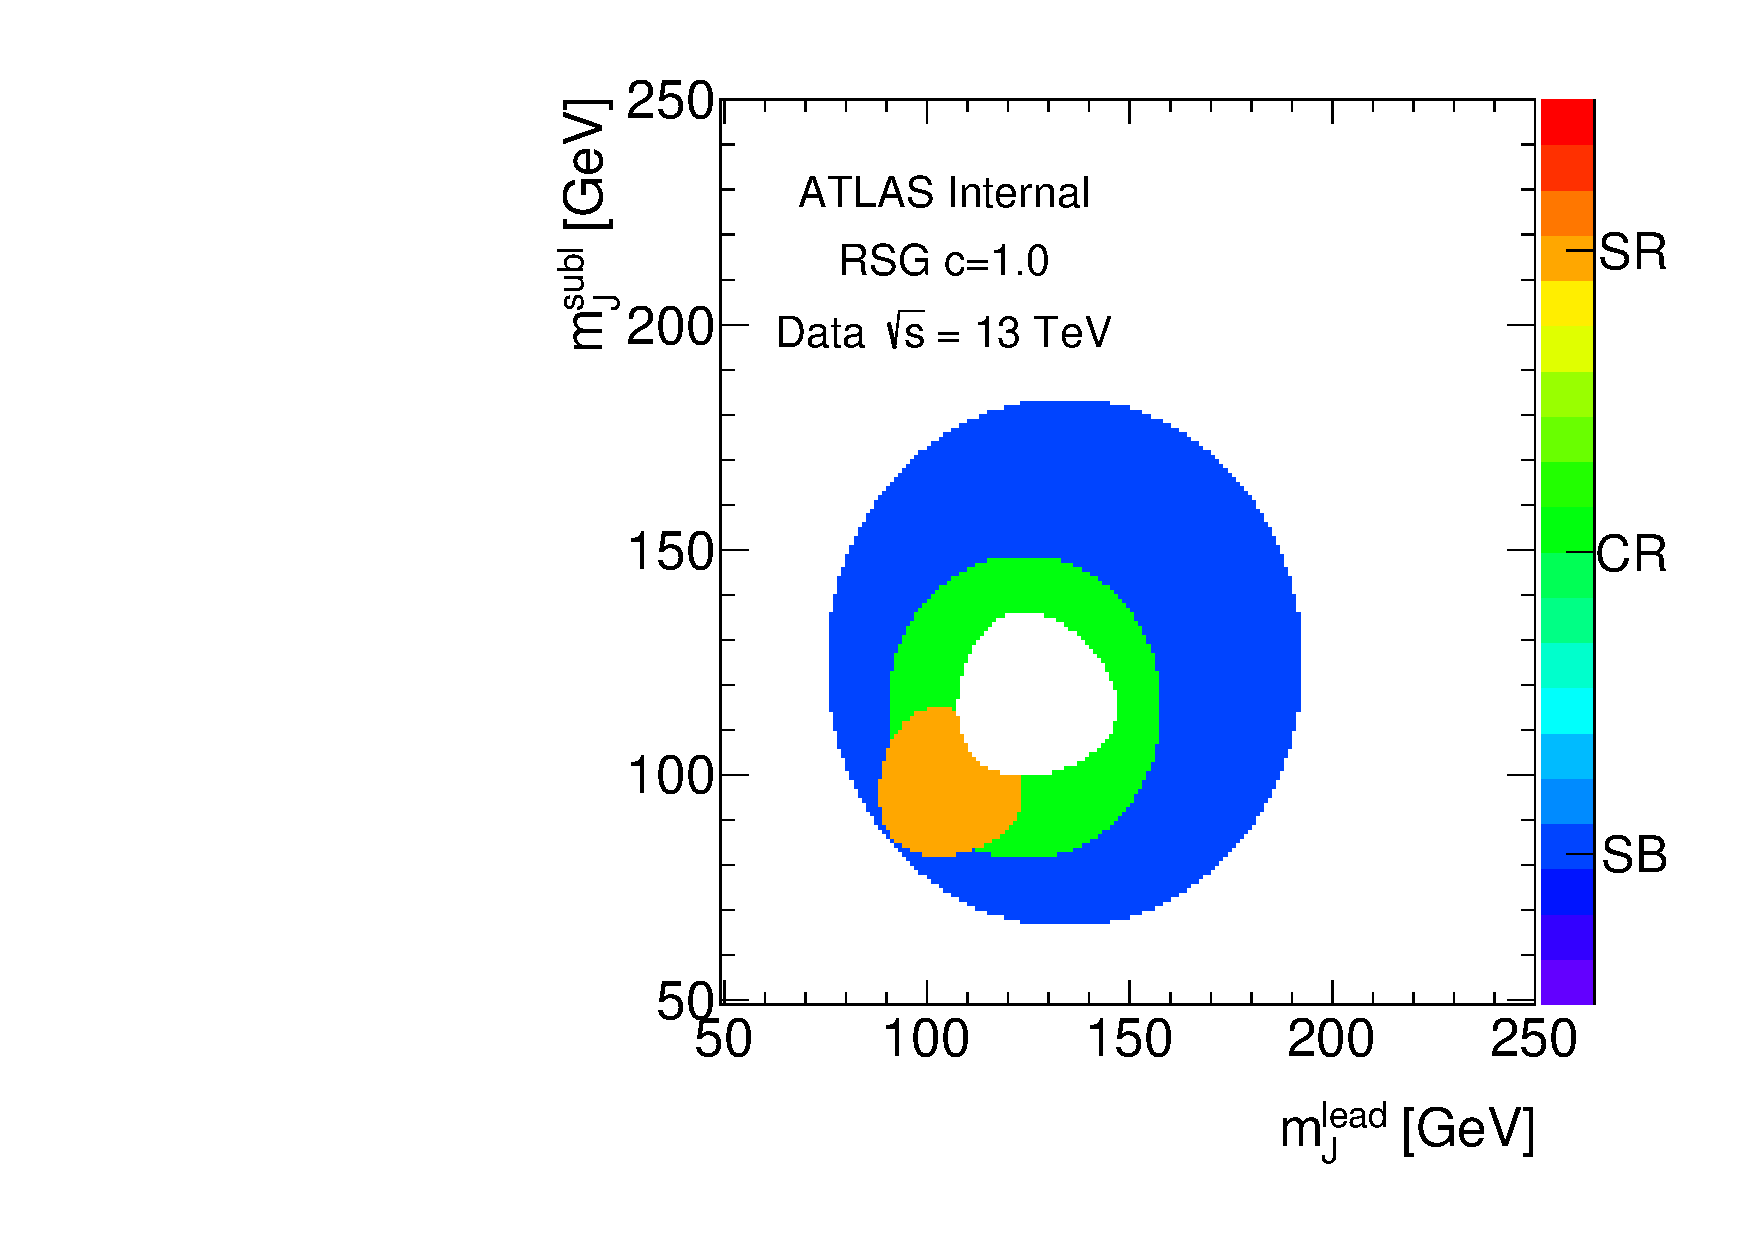
\includegraphics[width=0.4\textwidth,angle=-90]{figures/boosted/ZZ/Compare_NoTag_mH0H1.pdf}
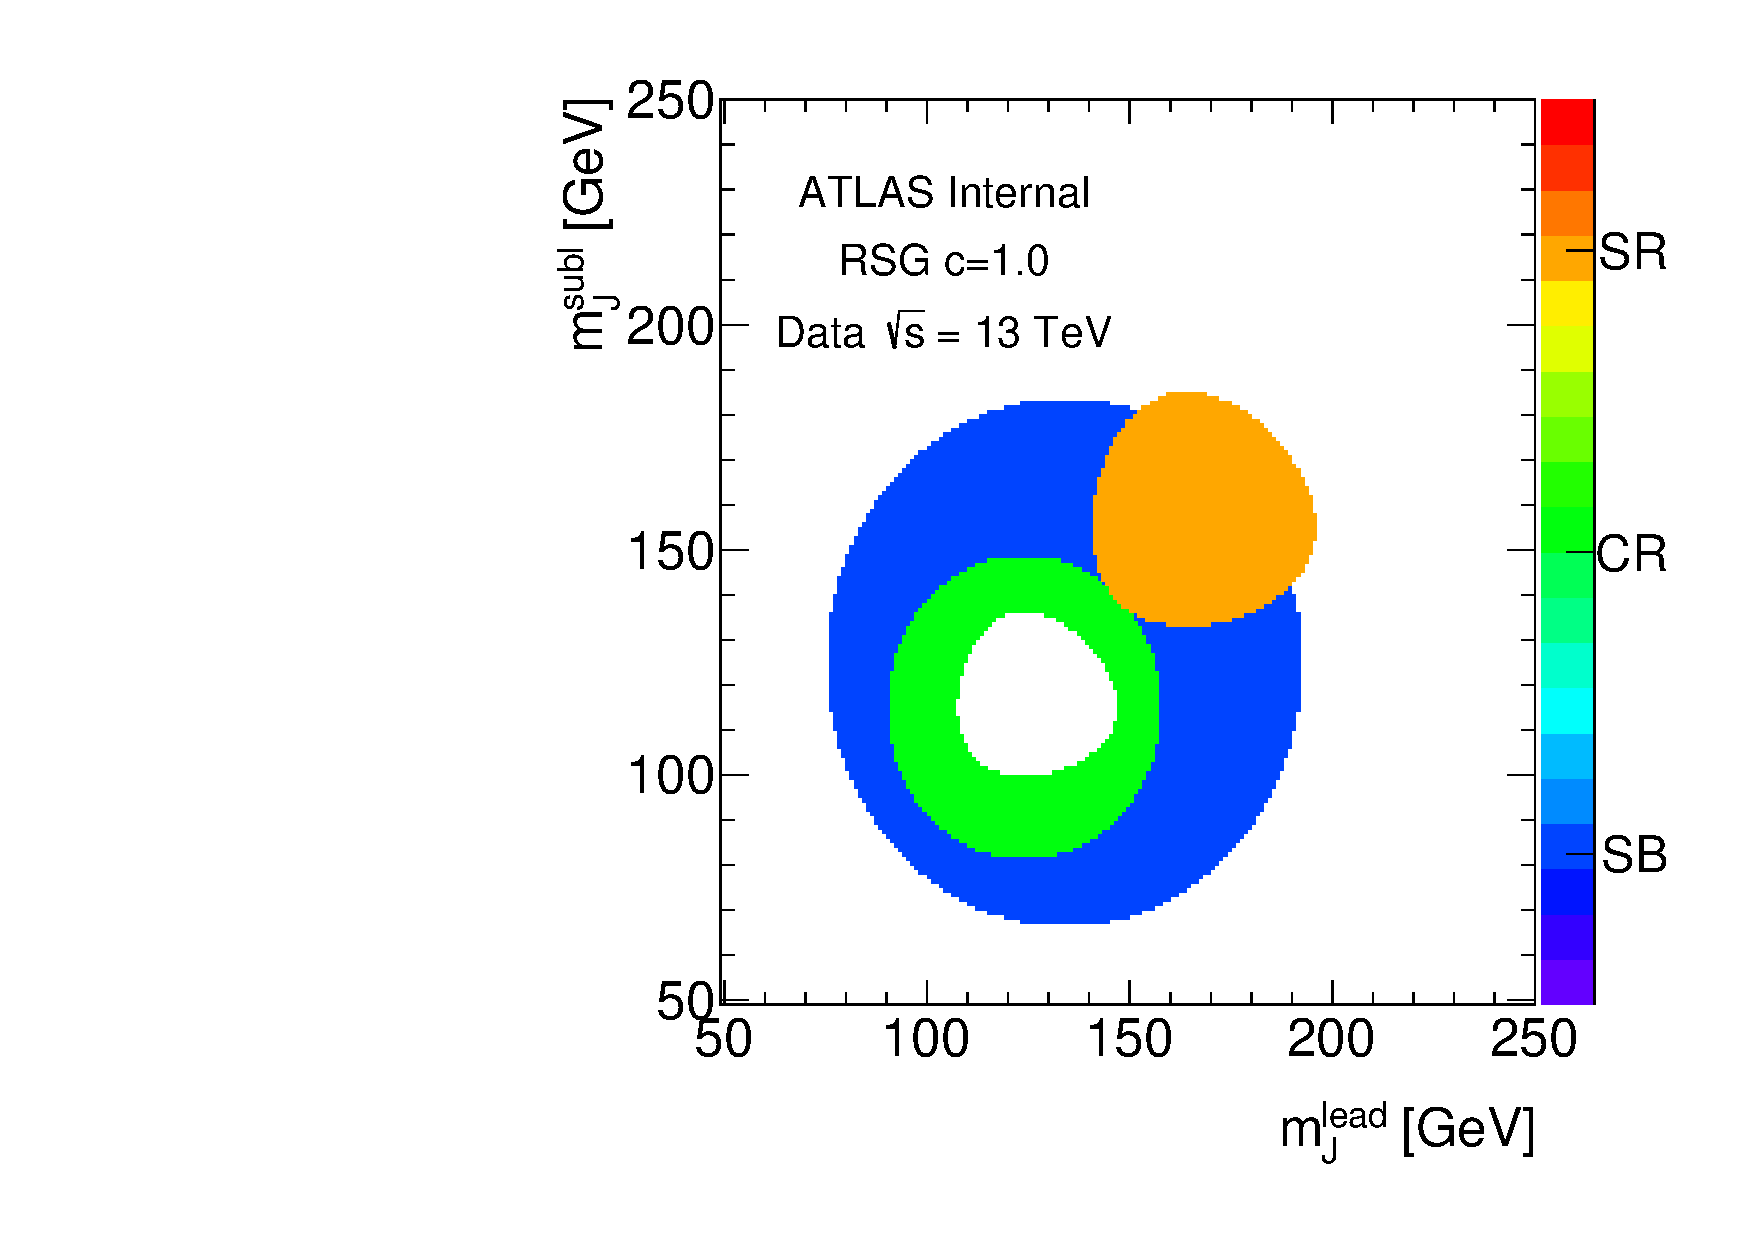
\includegraphics[width=0.4\textwidth,angle=-90]{figures/boosted/TT/Compare_NoTag_mH0H1.pdf}
\end{center}
\caption{Illustration of ZZ (left) and TT (right) signal region as shown in the orange shaded region. Control region shown in green, and Sideband region in blue. The white circle in the midde is the real Signal region, and it is blinded.}
\label{CRSB:ZZIllustration}
\end{figure}

%%\paragraph{}
The summary of background estimation for ZZ signal region can be found in Table \ref{CRSB:SummaryTable_ZZ_4b}, ~\ref{CRSB:SummaryTable_ZZ_3b} and ~\ref{CRSB:SummaryTable_ZZ_2b}. The difference between data and prediction in ZZ signal region is summarized in Table \ref{CRSB:DataPred_ZZSR} for all the regions. The discrepancy between data and prediction is either covered by statistical uncertainty of data or comparable with data statistical uncertainty in $4b$, $3b$ and $2bs$ ZZ SR respectively. We further check the kinematic distribution between data and prediction in ZZ SR, as shown in Figure \ref{CRSB:ZZSR_Distribution}. The data agrees with prediction well in general, though a few bins might not agree perfectly. The difference from $4b$ CR region test is 17$\%$, which is smaller than the $4b$ ZZ region difference. But the statistical uncertainty in ZZ region (yield 37) is much higher compared with our CR regions (min yield 76), hence the CR region with more statistical power is still used for the non-closure uncertainty.

%%\paragraph{}
The summary of background estimation for TT signal region can be found in Table \ref{CRSB:SummaryTable_TT_4b}, ~\ref{CRSB:SummaryTable_TT_3b} and ~\ref{CRSB:SummaryTable_TT_2b}. The difference between data and prediction in TT signal region is summarized in Table \ref{CRSB:DataPred_TTSR} for all the regions. The discrepancy between data and prediction is either covered by statistical uncertainty of data or comparable with data statistical uncertainty in $4b$, $3b$ and $2bs$ TT SR respectively. We further check the kinematic distribution between data and prediction in TT SR, as shown in Figure \ref{CRSB:TTSR_Distribution}. The data agrees with prediction well in general, though a few bins might not agree perfectly. 

%%\paragraph{}
Based on all the variation tests done above, we think there is no need to introduce extra uncertainty on non-closure systematics since most of the data/prediction disagreements are well covered by the data statistical uncertainty.

\begin{table}[htbp!]
\begin{center}
\begin{footnotesize} 
\begin{tabular}{c|c|c|c} 
FourTag & Sideband & Control & Signal \\ 
\hline\hline 
QCD Est & 166.65 $\pm$ 2.88 & 45.83 $\pm$ 1.51 & 27.37 $\pm$ 1.16\\ 
$t\bar{t}$ Est.  & 27.52 $\pm$ 0.25 & 6.31 $\pm$ 0.14 & 0 $\pm$ 0\\ 
$Z+jets$ & 0 $\pm$ 0 & 6.18 $\pm$ 5.12 & 0 $\pm$ 0\\ 
Total Bkg Est & 194.17 $\pm$ 2.89 & 58.32 $\pm$ 5.34 & 27.37 $\pm$ 1.16\\ 
Data & 194.0 $\pm$ 13.93 & 54.0 $\pm$ 7.35 & 37.0 $\pm$ 6.08\\ 
$c=1.0$,$m=1.0TeV$ & 2.45 $\pm$ 0.098 & 4.47 $\pm$ 0.13 & 0.99 $\pm$ 0.063\\ 
$c=1.0$,$m=2.0TeV$ & 0.032 $\pm$ 0.0015 & 0.075 $\pm$ 0.0022 & 0.028 $\pm$ 0.0014\\ 
$c=1.0$,$m=3.0TeV$ & 0.00029 $\pm$ 3.5e-05 & 0.00064 $\pm$ 5e-05 & 0.0002 $\pm$ 2.7e-05\\ 
\hline\hline 
\end{tabular} 
\end{footnotesize} 
\newline 

\end{center}
\caption{Background prediction in SR/CR/SB for ZZ SR in $4b$-tag region. Uncertainties are stat only.}
\label{CRSB:SummaryTable_ZZ_4b}
\end{table}

\begin{table}[htbp!]
\begin{center}
\begin{footnotesize} 
\begin{tabular}{c|c|c|c} 
ThreeTag & Sideband & Control & Signal \\ 
\hline\hline 
& & & \\ 
QCD Est & 3344.46 $\pm$ 26.85 & 998.41 $\pm$ 14.63 & 637.78 $\pm$ 11.87\\ 
$t\bar{t}$ Est.  & 826.66 $\pm$ 25.11 & 136.58 $\pm$ 10.23 & 30.07 $\pm$ 1.24\\ 
$Z+jets$ & 32.49 $\pm$ 11.34 & 8.22 $\pm$ 5.29 & 3.3 $\pm$ 2.0\\ 
Total Bkg Est & 4203.61 $\pm$ 38.47 & 1143.2 $\pm$ 18.62 & 671.15 $\pm$ 12.11\\ 
Data & 4203.0 $\pm$ 64.83 & 1108.0 $\pm$ 33.29 & 645.0 $\pm$ 25.4\\ 
$c=1.0$,$m=1.0TeV$ & 7.56 $\pm$ 0.18 & 9.84 $\pm$ 0.2 & 3.05 $\pm$ 0.11\\ 
$c=1.0$,$m=2.0TeV$ & 0.15 $\pm$ 0.0033 & 0.27 $\pm$ 0.0046 & 0.12 $\pm$ 0.003\\ 
$c=1.0$,$m=3.0TeV$ & 0.0034 $\pm$ 0.00012 & 0.0056 $\pm$ 0.00016 & 0.0021 $\pm$ 9.5e-05\\ 
& & & \\ 
\hline\hline 
\end{tabular} 
\end{footnotesize} 
\newline 

\end{center}
\caption{Background prediction in SR/CR/SB for ZZ SR in $3b$-tag region. Uncertainties are stat only.}
\label{CRSB:SummaryTable_ZZ_3b}
\end{table}

\begin{table}[htbp!]
\begin{center}
\begin{footnotesize} 
\begin{tabular}{c|c|c|c} 
TwoTag split & Sideband & Control & Signal \\ 
\hline\hline 
QCD Est & 16387.44 $\pm$ 37.6 & 4827.76 $\pm$ 19.86 & 3026.83 $\pm$ 15.61\\ 
$t\bar{t}$ Est.  & 7671.95 $\pm$ 69.14 & 1229.96 $\pm$ 26.54 & 332.29 $\pm$ 13.66\\ 
$Z+jets$ & 44.37 $\pm$ 13.23 & 13.34 $\pm$ 6.6 & 36.47 $\pm$ 12.88\\ 
Total Bkg Est & 24103.77 $\pm$ 79.8 & 6071.07 $\pm$ 33.8 & 3395.59 $\pm$ 24.42\\ 
Data & 24104.0 $\pm$ 155.25 & 6261.0 $\pm$ 79.13 & 3258.0 $\pm$ 57.08\\ 
$c=1.0$,$m=1.0TeV$ & 4.57 $\pm$ 0.14 & 4.65 $\pm$ 0.14 & 1.91 $\pm$ 0.089\\ 
$c=1.0$,$m=2.0TeV$ & 0.16 $\pm$ 0.0038 & 0.26 $\pm$ 0.0047 & 0.12 $\pm$ 0.0032\\ 
$c=1.0$,$m=3.0TeV$ & 0.012 $\pm$ 0.00024 & 0.019 $\pm$ 0.00029 & 0.0085 $\pm$ 0.00019\\ 
\hline\hline 
\end{tabular} 
\end{footnotesize} 
\newline 

\end{center}
\caption{Background prediction in SR/CR/SB for ZZ SR in $2bs$-tag region. Uncertainties are stat only.}
\label{CRSB:SummaryTable_ZZ_2b}
\end{table}

\begin{table}[htbp!]
\begin{center}
\begin{footnotesize} 
\begin{tabular}{c|c|c|c} 
ZZ Signal Region & Data & Prediction & (Predict - Data)/Data \\ 
\hline\hline 
FourTag & 37.0 $\pm$ 6.08 & 27.37 $\pm$ 1.16 & -26.0 $\%$  $\pm$ 15.3 $\%$ \\ 
\hline 
ThreeTag & 645.0 $\pm$ 25.4 & 671.15 $\pm$ 12.11 & 4.05 $\%$  $\pm$ 5.97 $\%$ \\ 
\hline 
TwoTag split & 3258.0 $\pm$ 57.08 & 3395.59 $\pm$ 24.42 & 4.22 $\%$  $\pm$ 2.58 $\%$ \\ 
\hline\hline 
\end{tabular} 
\end{footnotesize} 
\newline 

\end{center}
\caption{Agreement between data and prediction in ZZ SR in $4b$, $3b$ and $2bs$ regions.}
\label{CRSB:DataPred_ZZSR}
\end{table}

\begin{figure}[htbp!]
\begin{center}
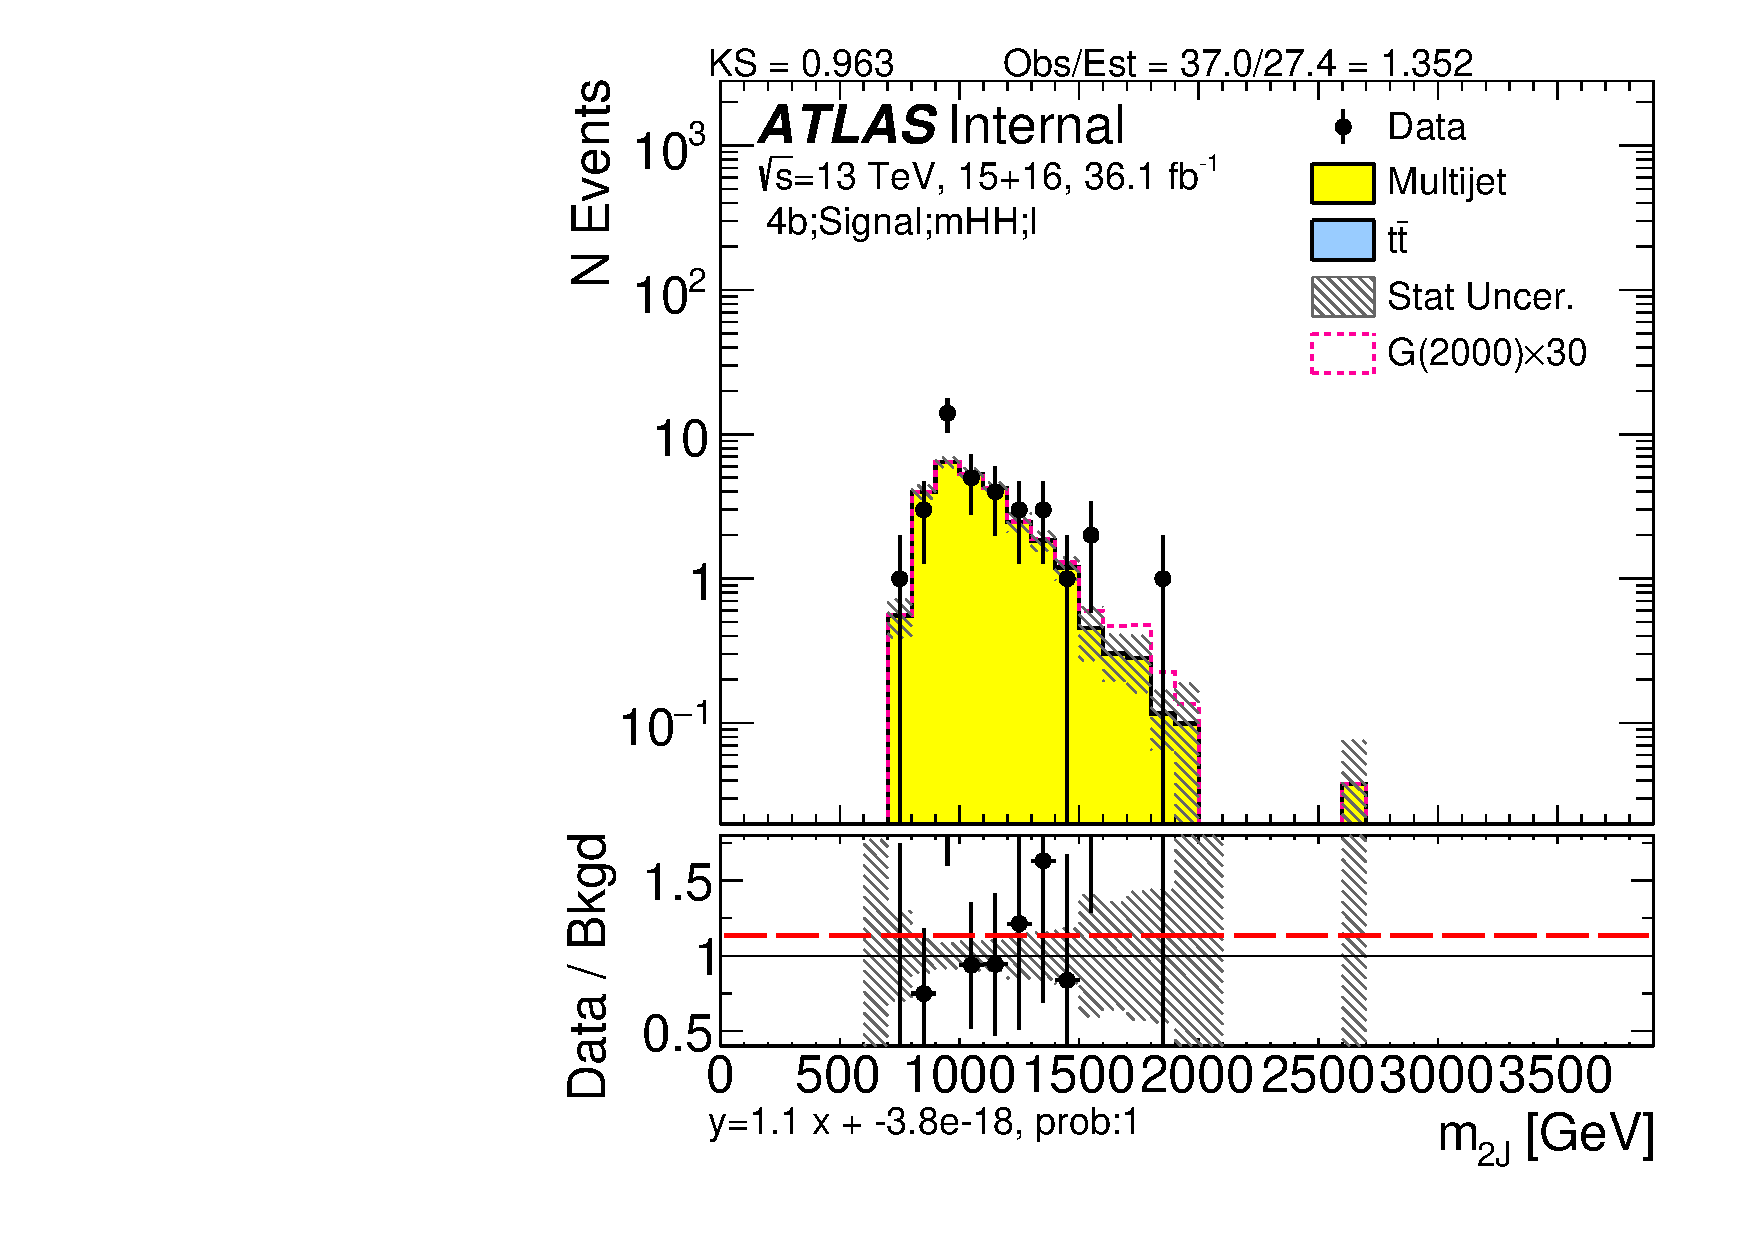
\includegraphics[width=0.45\textwidth,angle=-90]{figures/boosted/ZZ/Moriond_ZZ_FourTag_Signal_mHH_l_1.pdf}
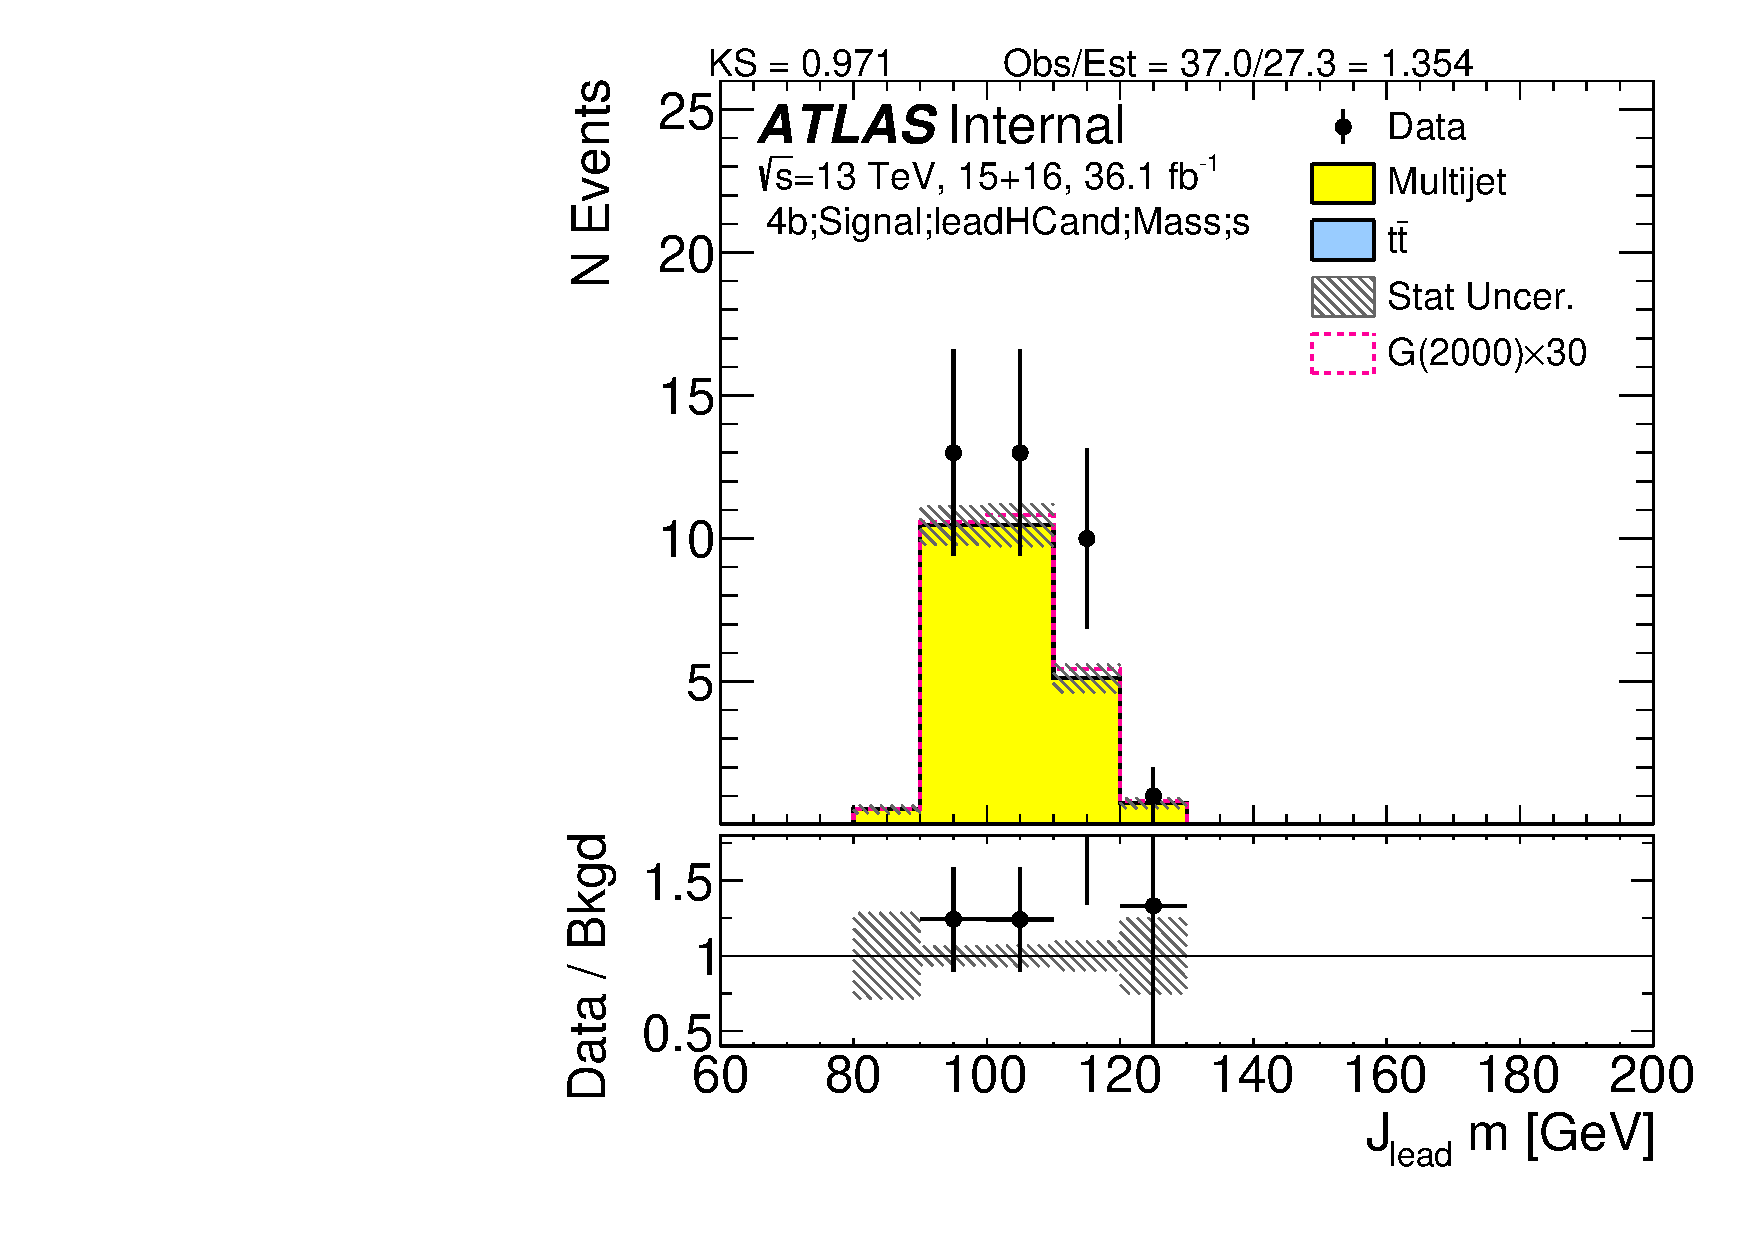
\includegraphics[width=0.45\textwidth,angle=-90]{figures/boosted/ZZ/Moriond_ZZ_FourTag_Signal_leadHCand_Mass_s.pdf}\\
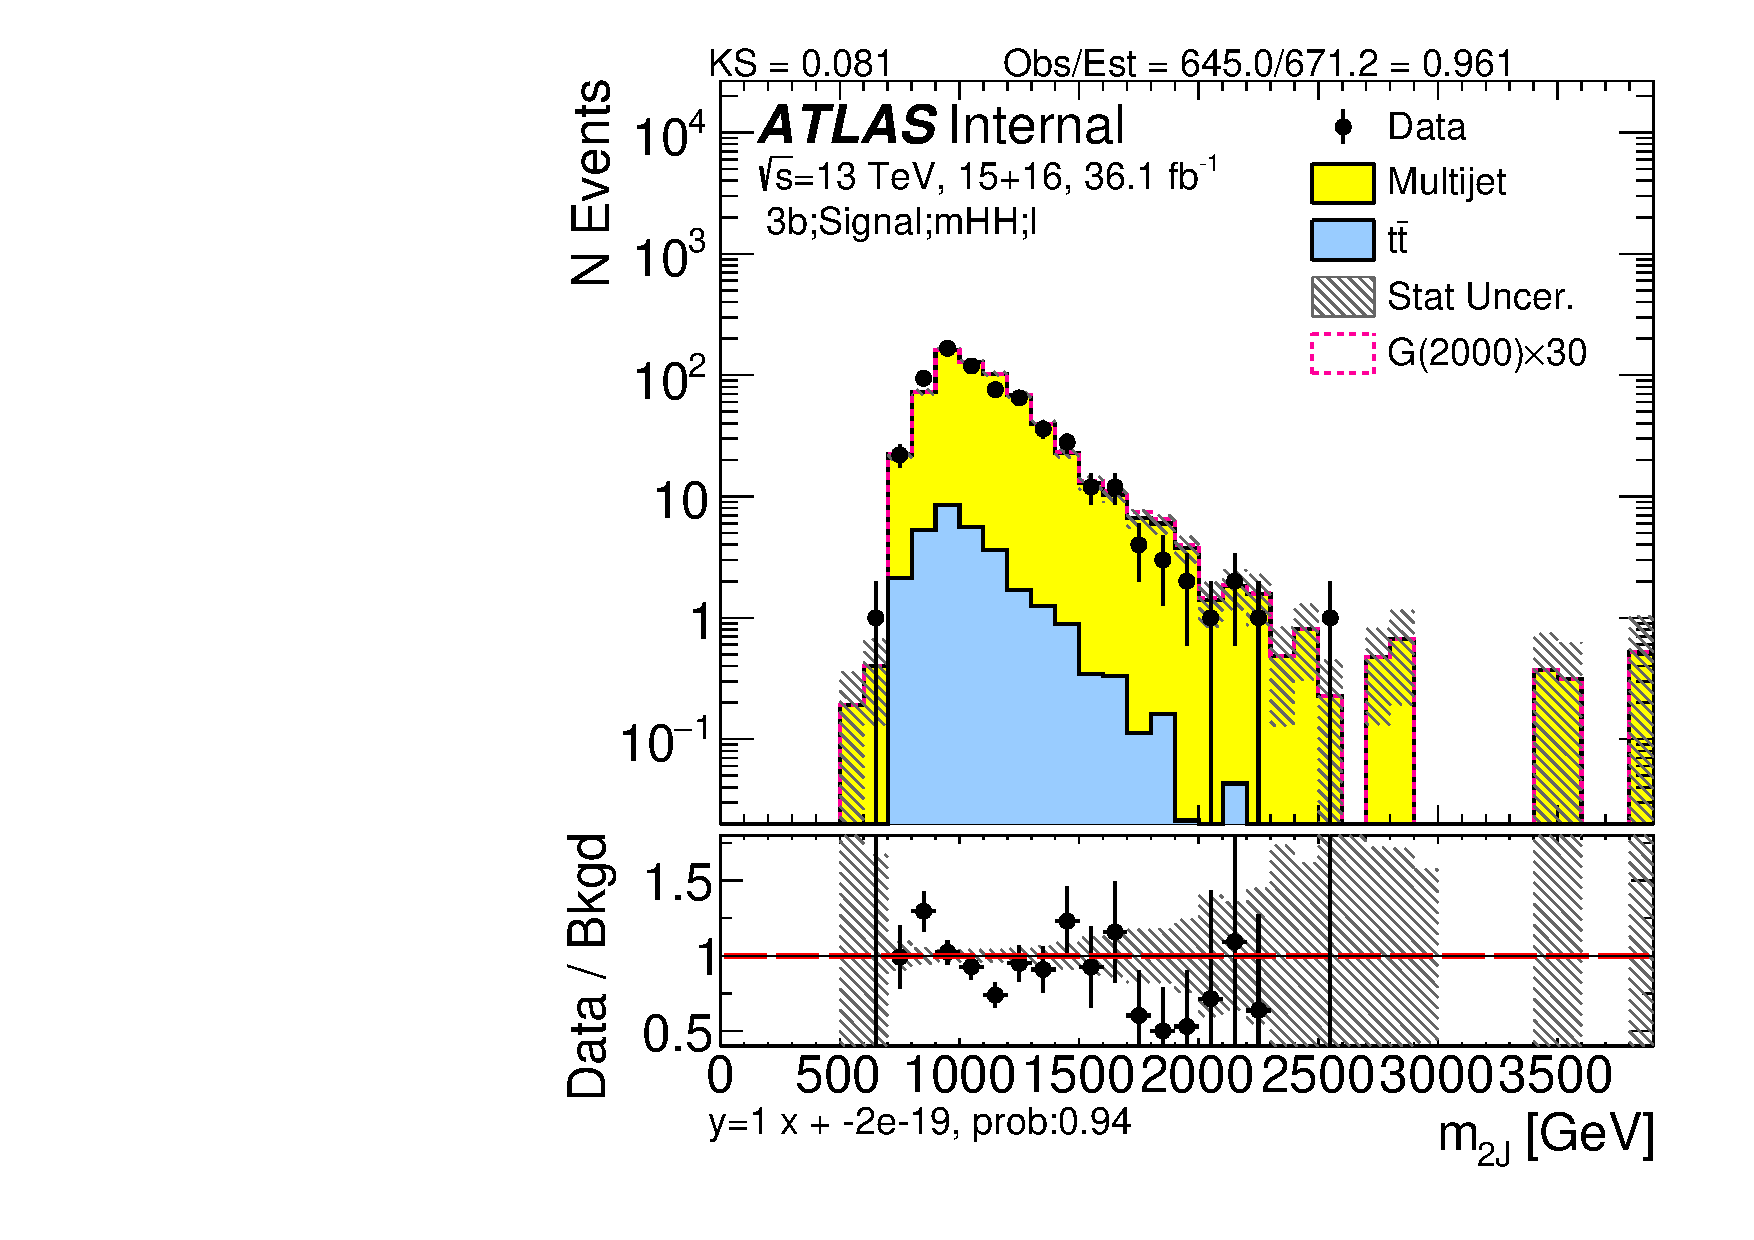
\includegraphics[width=0.45\textwidth,angle=-90]{figures/boosted/ZZ/Moriond_ZZ_ThreeTag_Signal_mHH_l_1.pdf}
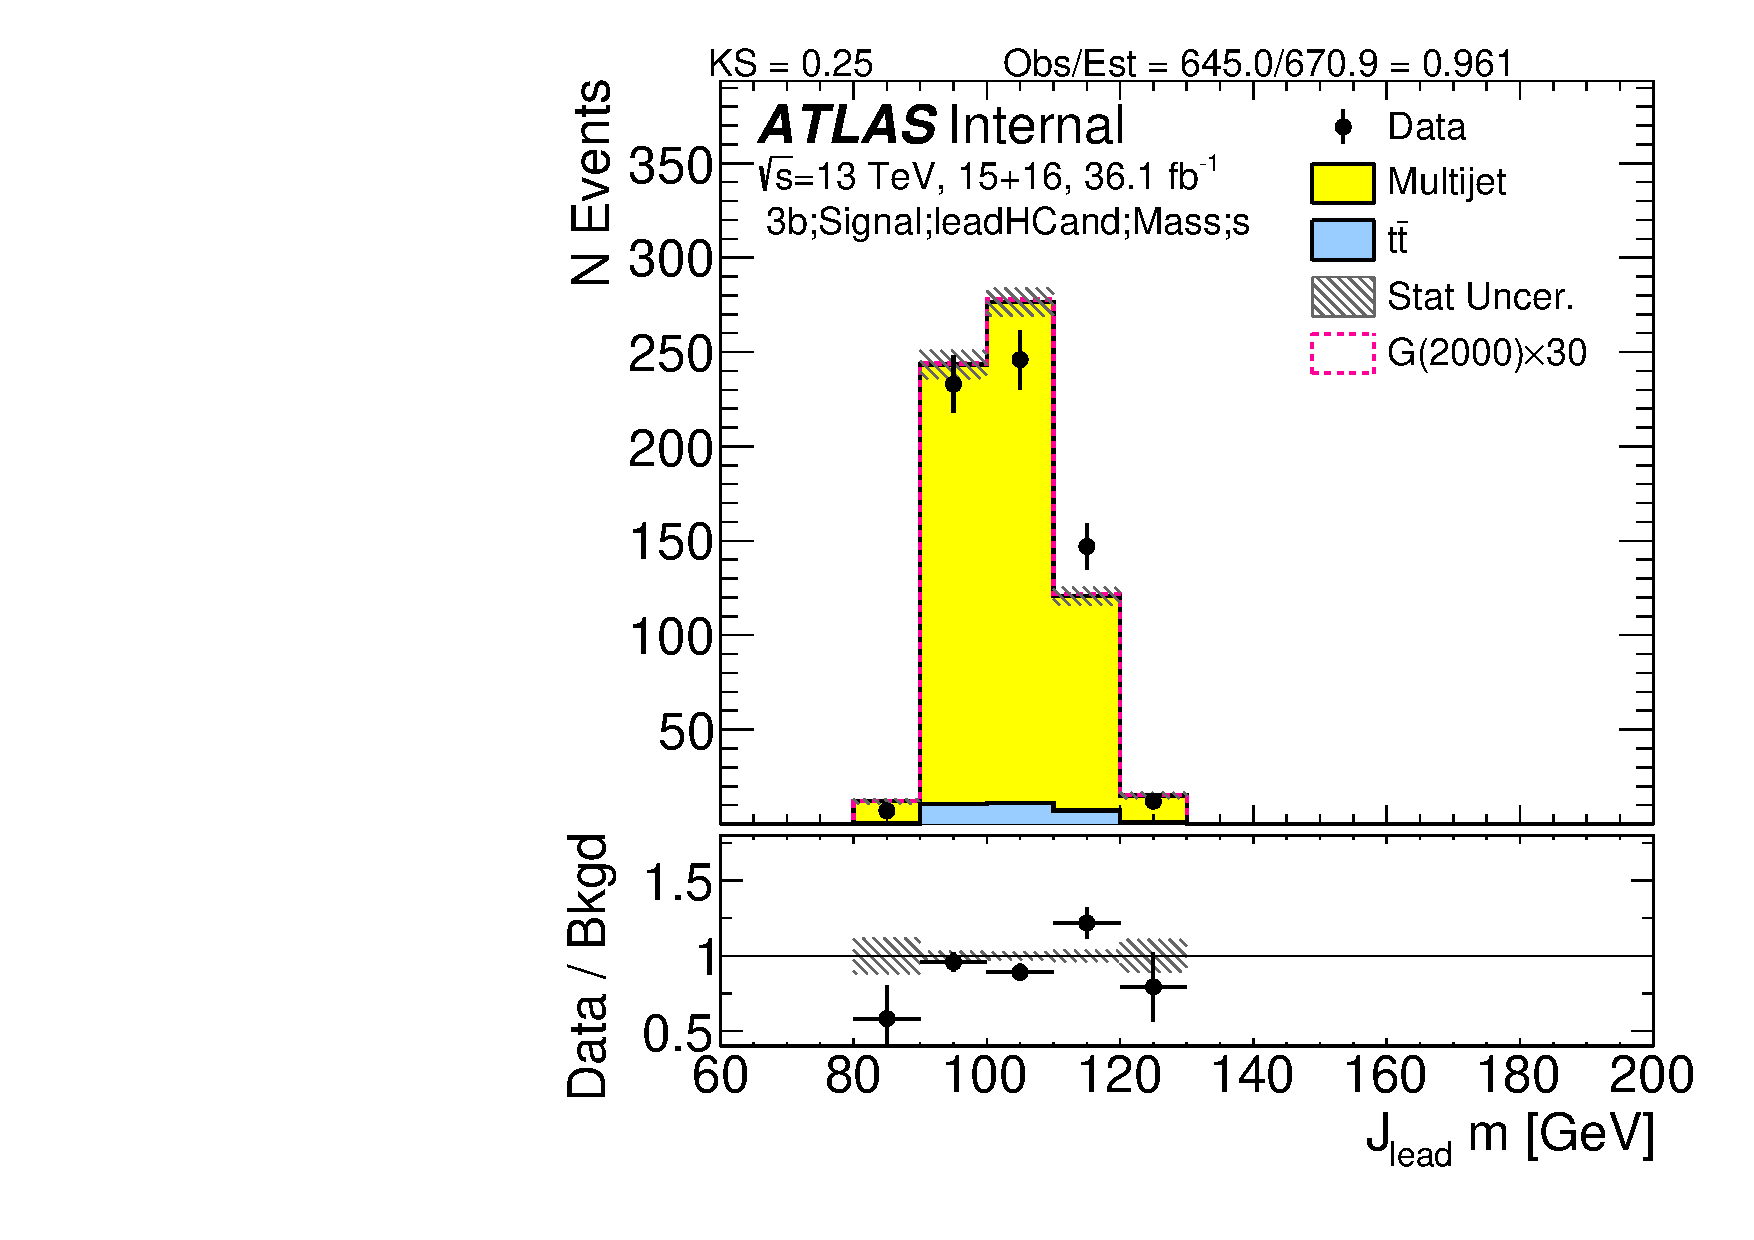
\includegraphics[width=0.45\textwidth,angle=-90]{figures/boosted/ZZ/Moriond_ZZ_ThreeTag_Signal_leadHCand_Mass_s.pdf}\\
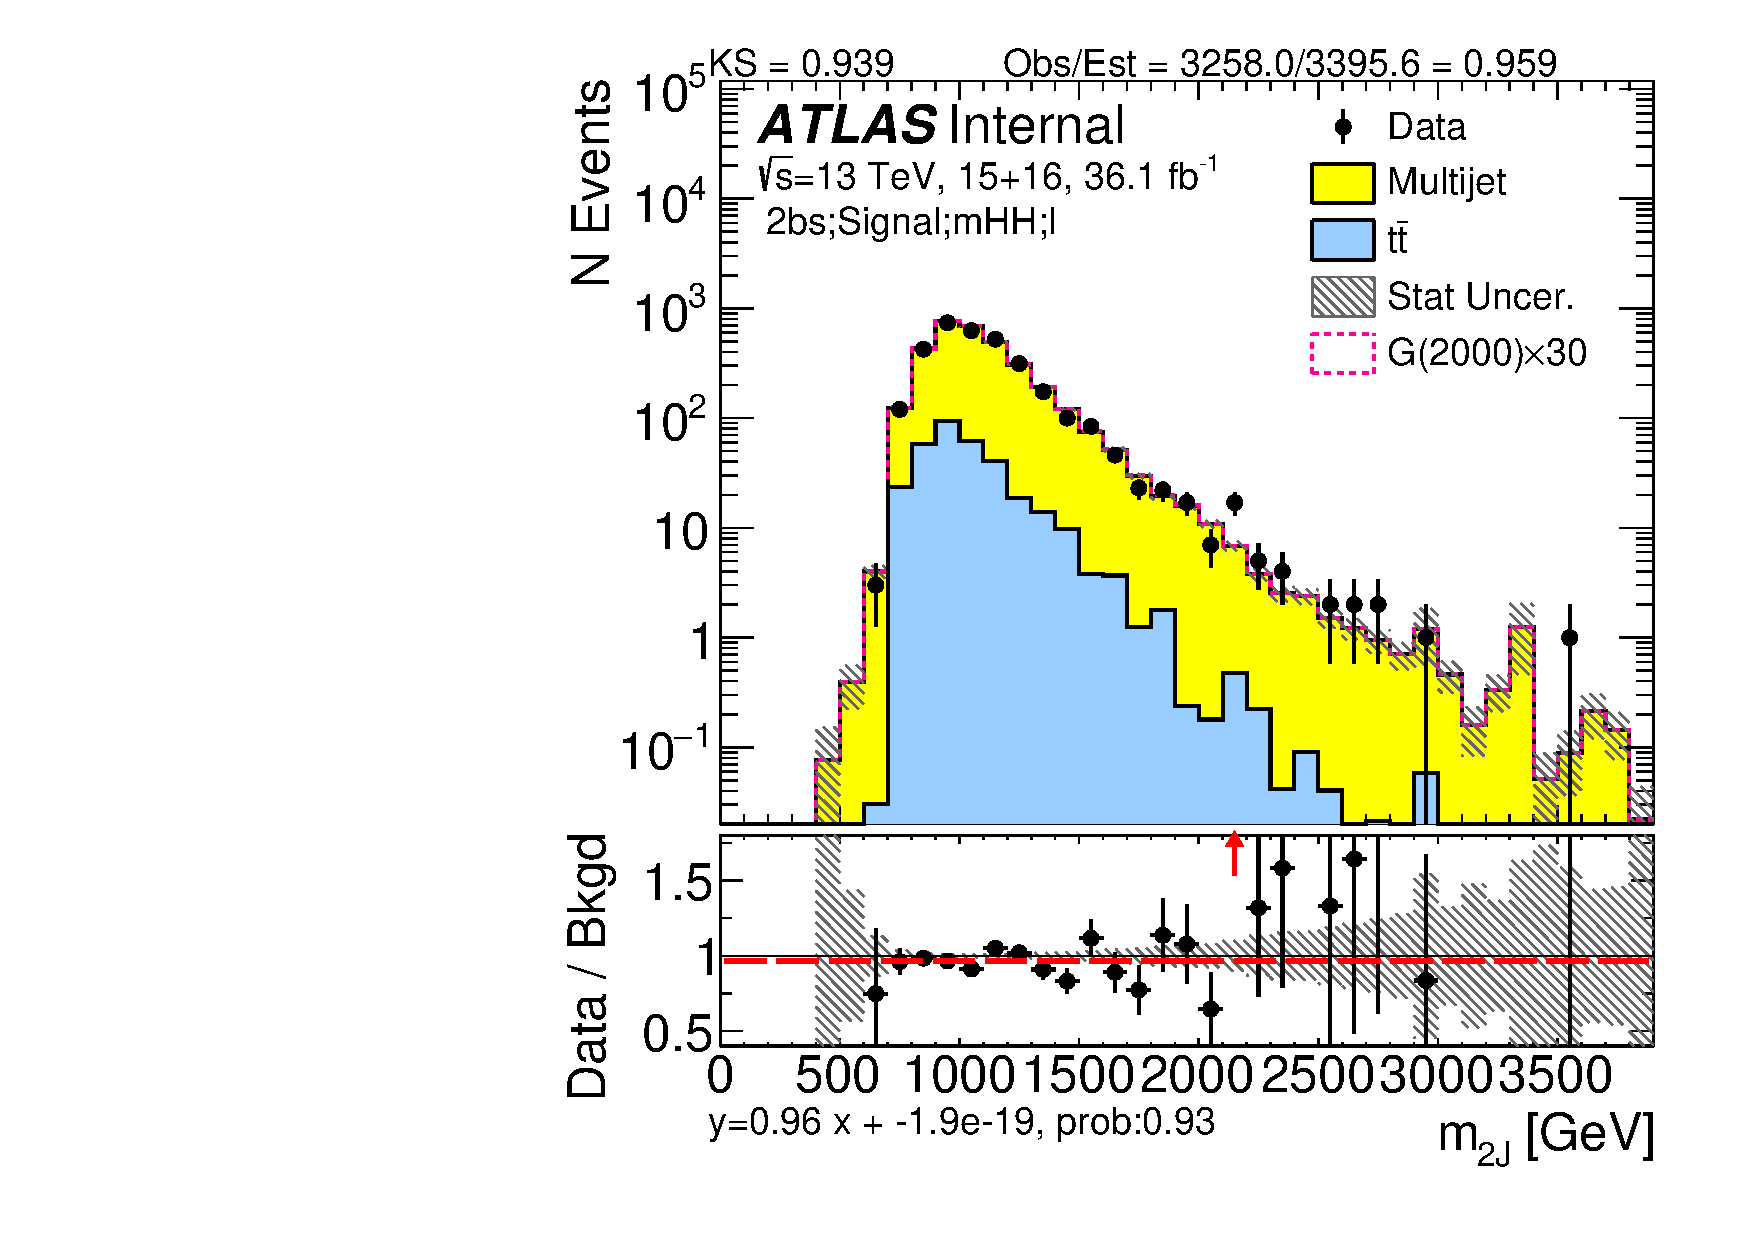
\includegraphics[width=0.45\textwidth,angle=-90]{figures/boosted/ZZ/Moriond_ZZ_TwoTag_split_Signal_mHH_l_1.pdf}
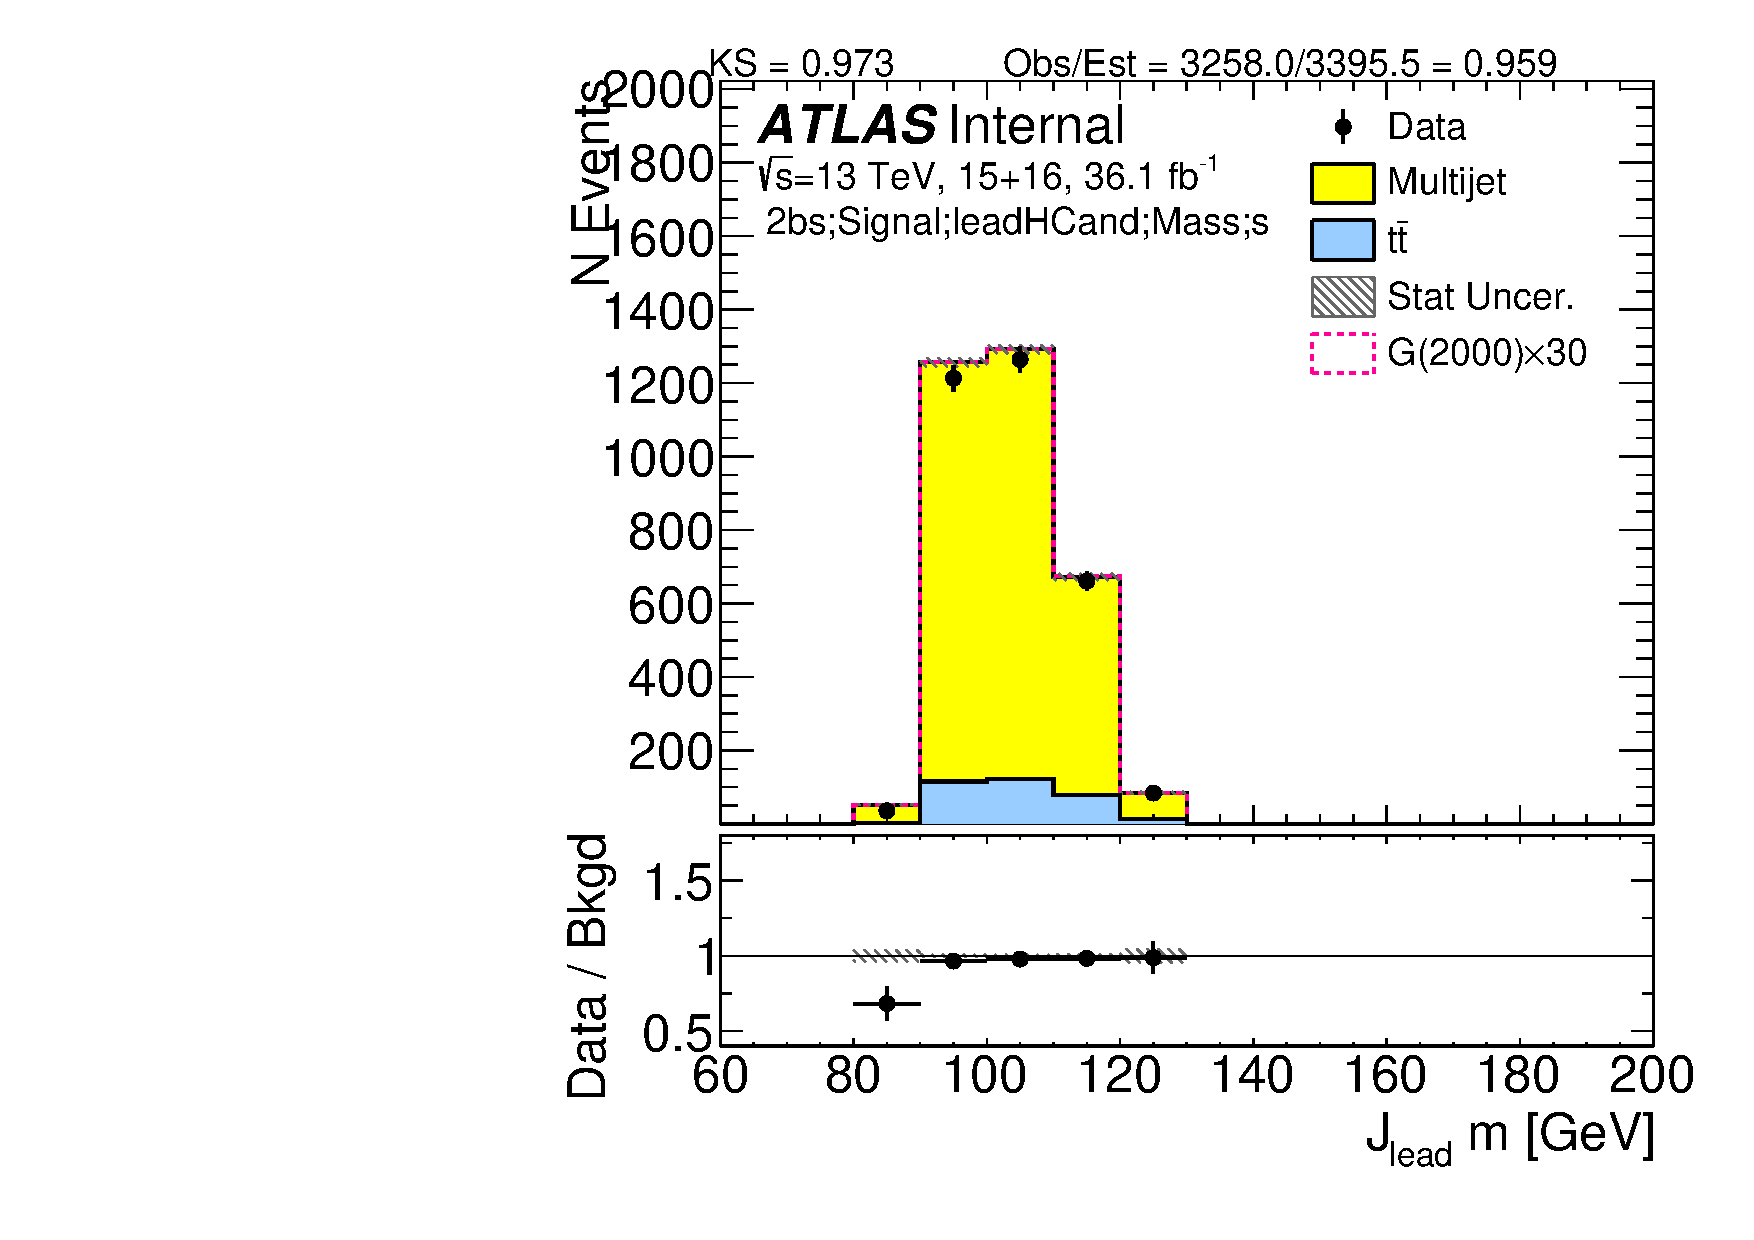
\includegraphics[width=0.45\textwidth,angle=-90]{figures/boosted/ZZ/Moriond_ZZ_TwoTag_split_Signal_leadHCand_Mass_s.pdf}\\
\end{center}
\caption{ZZ signal region distribution of di-jet mass (left column) and leading large-R jet mass (right column) in low mass signal, for $4b$ (top row), $3b$(middle row) and $2b$ split (bottom row). The plots are with only statistical uncertainty.}
\label{CRSB:ZZSR_Distribution}
\end{figure}

\begin{table}[htbp!]
\begin{center}
\begin{footnotesize} 
\begin{tabular}{c|c|c|c} 
FourTag & Sideband & Control & Signal \\ 
\hline\hline 
& & & \\ 
QCD Est & 152.28 $\pm$ 2.72 & 63.47 $\pm$ 1.77 & 28.6 $\pm$ 1.21\\ 
$t\bar{t}$ Est.  & 19.86 $\pm$ 0.22 & 7.45 $\pm$ 0.15 & 15.02 $\pm$ 0.2\\ 
$Z+jets$ & 0 $\pm$ 0 & 6.18 $\pm$ 5.12 & 0 $\pm$ 0\\ 
Total Bkg Est & 172.14 $\pm$ 2.73 & 77.1 $\pm$ 5.42 & 43.62 $\pm$ 1.23\\ 
Data & 172.0 $\pm$ 13.11 & 81.0 $\pm$ 9.0 & 46.0 $\pm$ 6.78\\ 
$c=1.0$,$m=1.0TeV$ & 2.38 $\pm$ 0.097 & 5.4 $\pm$ 0.15 & 0.15 $\pm$ 0.024\\ 
$c=1.0$,$m=2.0TeV$ & 0.033 $\pm$ 0.0015 & 0.1 $\pm$ 0.0026 & 0.0011 $\pm$ 0.00027\\ 
$c=1.0$,$m=3.0TeV$ & 0.00031 $\pm$ 3.6e-05 & 0.0008 $\pm$ 5.6e-05 & 1.5e-05 $\pm$ 7.7e-06\\ 
& & & \\ 
\hline\hline 
\end{tabular} 
\end{footnotesize} 
\newline 

\end{center}
\caption{Background prediction in SR/CR/SB for TT SR in $4b$-tag region. Uncertainties are stat only.}
\label{CRSB:SummaryTable_TT_4b}
\end{table}

\begin{table}[htbp!]
\begin{center}
\begin{footnotesize} 
\begin{tabular}{c|c|c|c} 
ThreeTag & Sideband & Control & Signal \\ 
\hline\hline 
QCD Est & 3106.11 $\pm$ 25.79 & 1427.41 $\pm$ 17.53 & 570.01 $\pm$ 11.6\\ 
$t\bar{t}$ Est.  & 495.21 $\pm$ 18.75 & 148.55 $\pm$ 10.21 & 406.57 $\pm$ 5.42\\ 
$Z+jets$ & 32.5 $\pm$ 11.34 & 11.21 $\pm$ 5.65 & 0.3 $\pm$ 0.3\\ 
Total Bkg Est & 3633.82 $\pm$ 33.85 & 1587.17 $\pm$ 21.05 & 976.88 $\pm$ 12.81\\ 
Data & 3633.0 $\pm$ 60.27 & 1553.0 $\pm$ 39.41 & 1017.0 $\pm$ 31.89\\ 
$c=1.0$,$m=1.0TeV$ & 7.57 $\pm$ 0.18 & 12.58 $\pm$ 0.23 & 0.32 $\pm$ 0.037\\ 
$c=1.0$,$m=2.0TeV$ & 0.15 $\pm$ 0.0034 & 0.38 $\pm$ 0.0054 & 0.0047 $\pm$ 0.0006\\ 
$c=1.0$,$m=3.0TeV$ & 0.0034 $\pm$ 0.00012 & 0.0075 $\pm$ 0.00018 & 0.00023 $\pm$ 3.3e-05\\ 
\hline\hline 
\end{tabular} 
\end{footnotesize} 
\newline 

\end{center}
\caption{Background prediction in SR/CR/SB for TT SR in $3b$-tag region. Uncertainties are stat only.}
\label{CRSB:SummaryTable_TT_3b}
\end{table}

\begin{table}[htbp!]
\begin{center}
\begin{footnotesize} 
\begin{tabular}{c|c|c|c} 
TwoTag split & Sideband & Control & Signal \\ 
\hline\hline 
QCD Est & 14980.05 $\pm$ 35.33 & 6803.06 $\pm$ 23.41 & 2817.92 $\pm$ 16.54\\ 
$t\bar{t}$ Est.  & 5170.92 $\pm$ 56.22 & 1468.85 $\pm$ 28.93 & 3628.91 $\pm$ 48.42\\ 
$Z+jets$ & 61.34 $\pm$ 16.04 & 26.44 $\pm$ 10.08 & 6.4 $\pm$ 5.05\\ 
Total Bkg Est & 20212.31 $\pm$ 68.31 & 8298.34 $\pm$ 38.56 & 6453.23 $\pm$ 51.41\\ 
Data & 20212.0 $\pm$ 142.17 & 8486.0 $\pm$ 92.12 & 6446.0 $\pm$ 80.29\\ 
$c=1.0$,$m=1.0TeV$ & 4.59 $\pm$ 0.14 & 6.33 $\pm$ 0.16 & 0.24 $\pm$ 0.033\\ 
$c=1.0$,$m=2.0TeV$ & 0.17 $\pm$ 0.0039 & 0.36 $\pm$ 0.0056 & 0.0066 $\pm$ 0.00077\\ 
$c=1.0$,$m=3.0TeV$ & 0.012 $\pm$ 0.00024 & 0.027 $\pm$ 0.00034 & 0.00089 $\pm$ 6.7e-05\\ 
\hline\hline 
\end{tabular} 
\end{footnotesize} 
\newline 

\end{center}
\caption{Background prediction in SR/CR/SB for TT SR in $2bs$-tag region. Uncertainties are stat only.}
\label{CRSB:SummaryTable_TT_2b}
\end{table}

\begin{table}[htbp!]
\begin{center}
\begin{footnotesize} 
\begin{tabular}{c|c|c|c} 
TT Signal Region & Data & Prediction & (Predict - Data)/Data \\ 
\hline\hline 
FourTag & 46.0 $\pm$ 6.78 & 43.62 $\pm$ 1.23 & -5.18 $\%$  $\pm$ 16.66 $\%$ \\ 
\hline 
ThreeTag & 1017.0 $\pm$ 31.89 & 976.88 $\pm$ 12.81 & -3.95 $\%$  $\pm$ 4.27 $\%$ \\ 
\hline 
TwoTag split & 6446.0 $\pm$ 80.29 & 6453.23 $\pm$ 51.41 & 0.11 $\%$  $\pm$ 2.04 $\%$ \\ 
\hline\hline 
\end{tabular} 
\end{footnotesize} 
\newline 

\end{center}
\caption{Agreement between data and prediction in TT SR in $4b$, $3b$ and $2bs$ regions.}
\label{CRSB:DataPred_TTSR}
\end{table}


\begin{figure}[htbp!]
\begin{center}
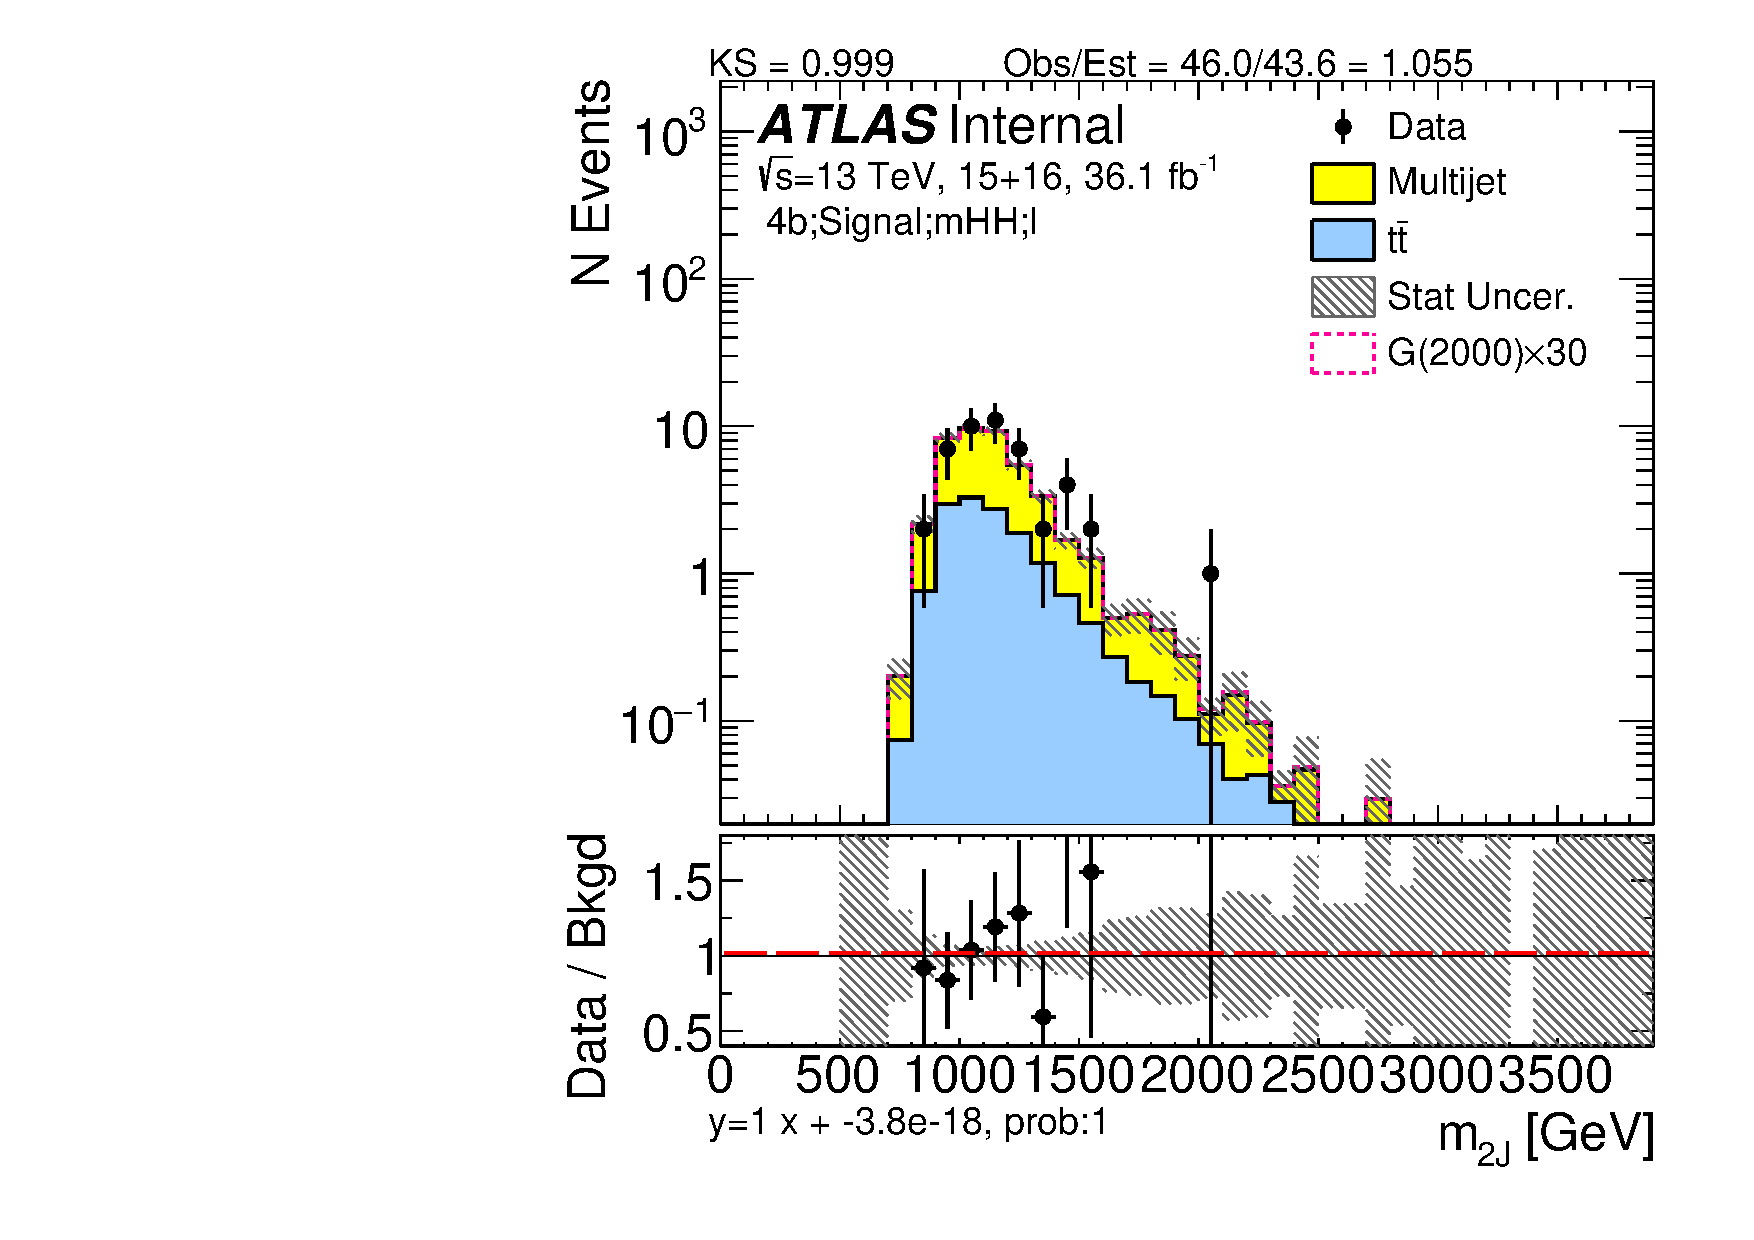
\includegraphics[width=0.45\textwidth,angle=-90]{figures/boosted/TT/Moriond_TT_FourTag_Signal_mHH_l_1.pdf}
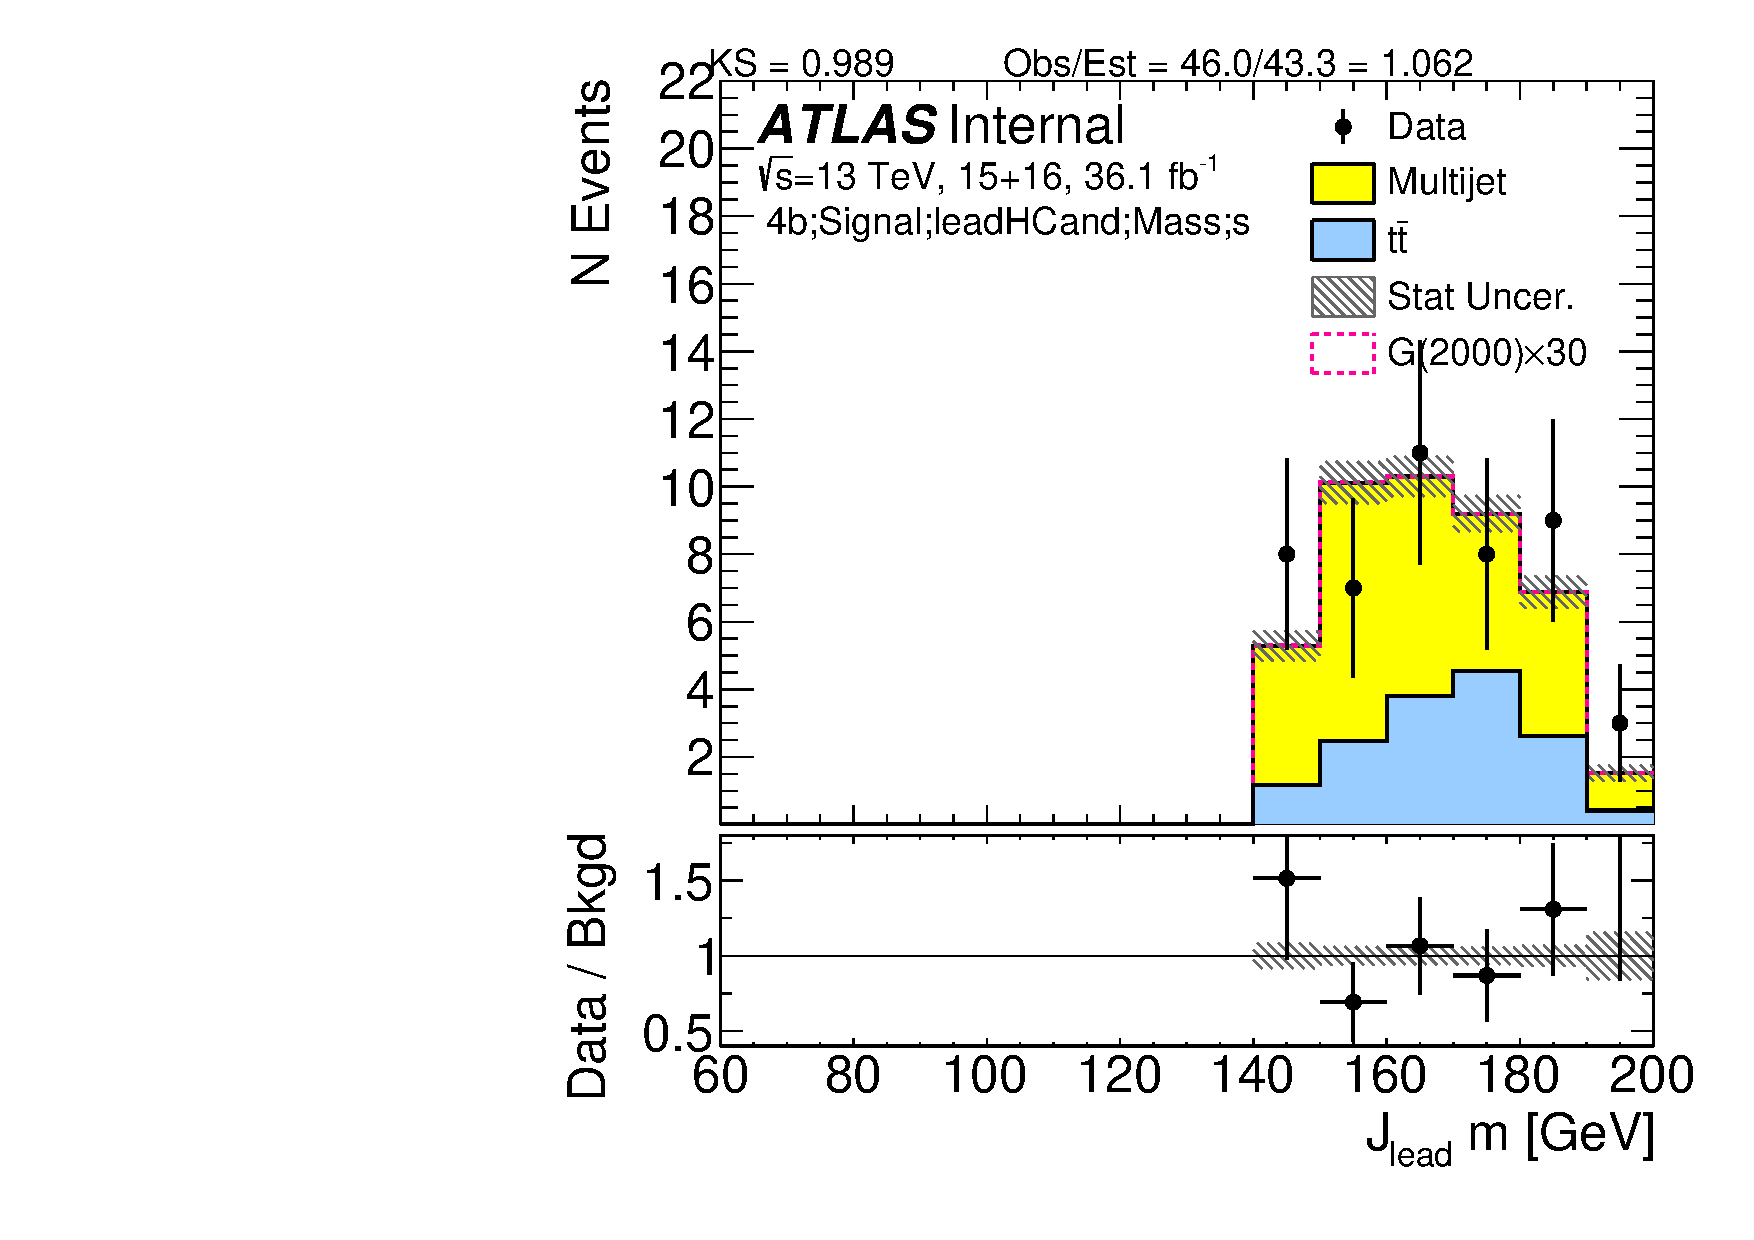
\includegraphics[width=0.45\textwidth,angle=-90]{figures/boosted/TT/Moriond_TT_FourTag_Signal_leadHCand_Mass_s.pdf}\\
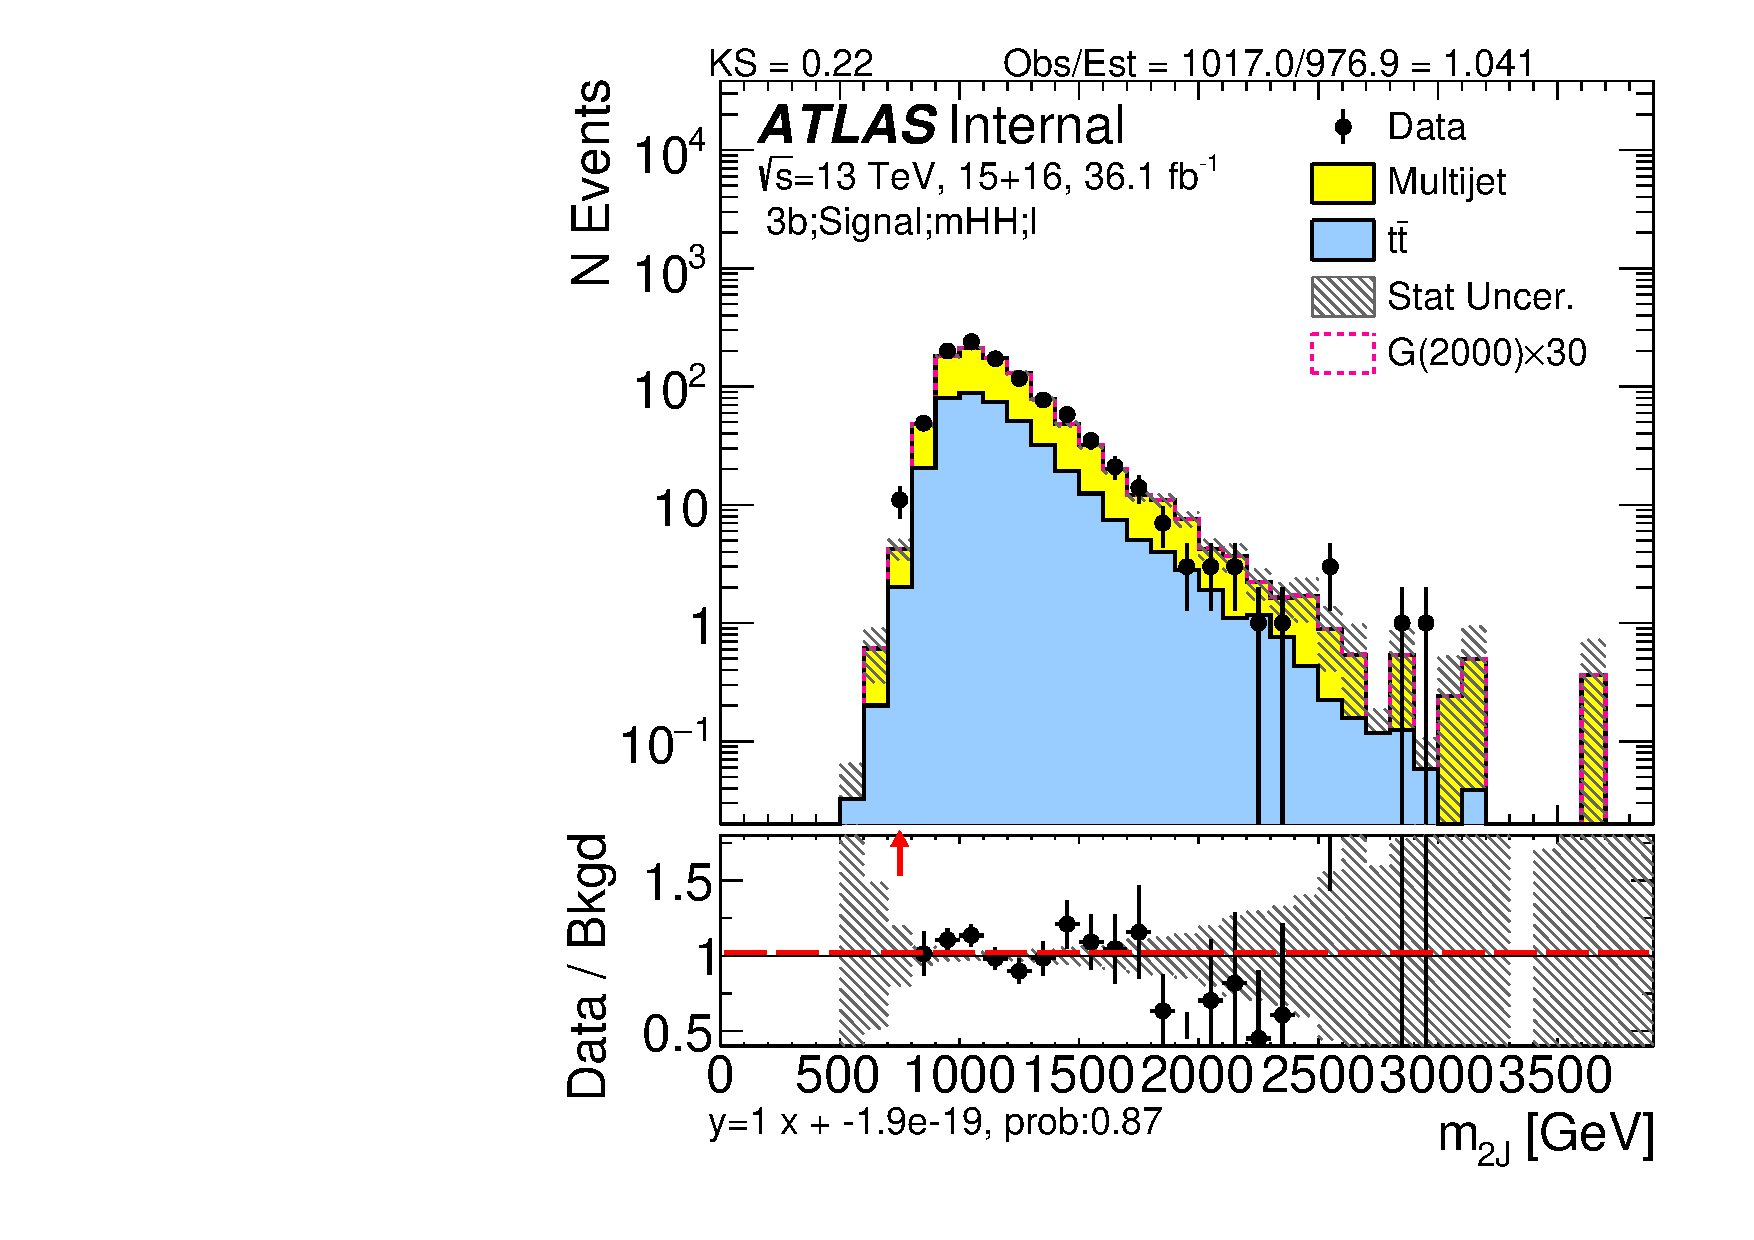
\includegraphics[width=0.45\textwidth,angle=-90]{figures/boosted/TT/Moriond_TT_ThreeTag_Signal_mHH_l_1.pdf}
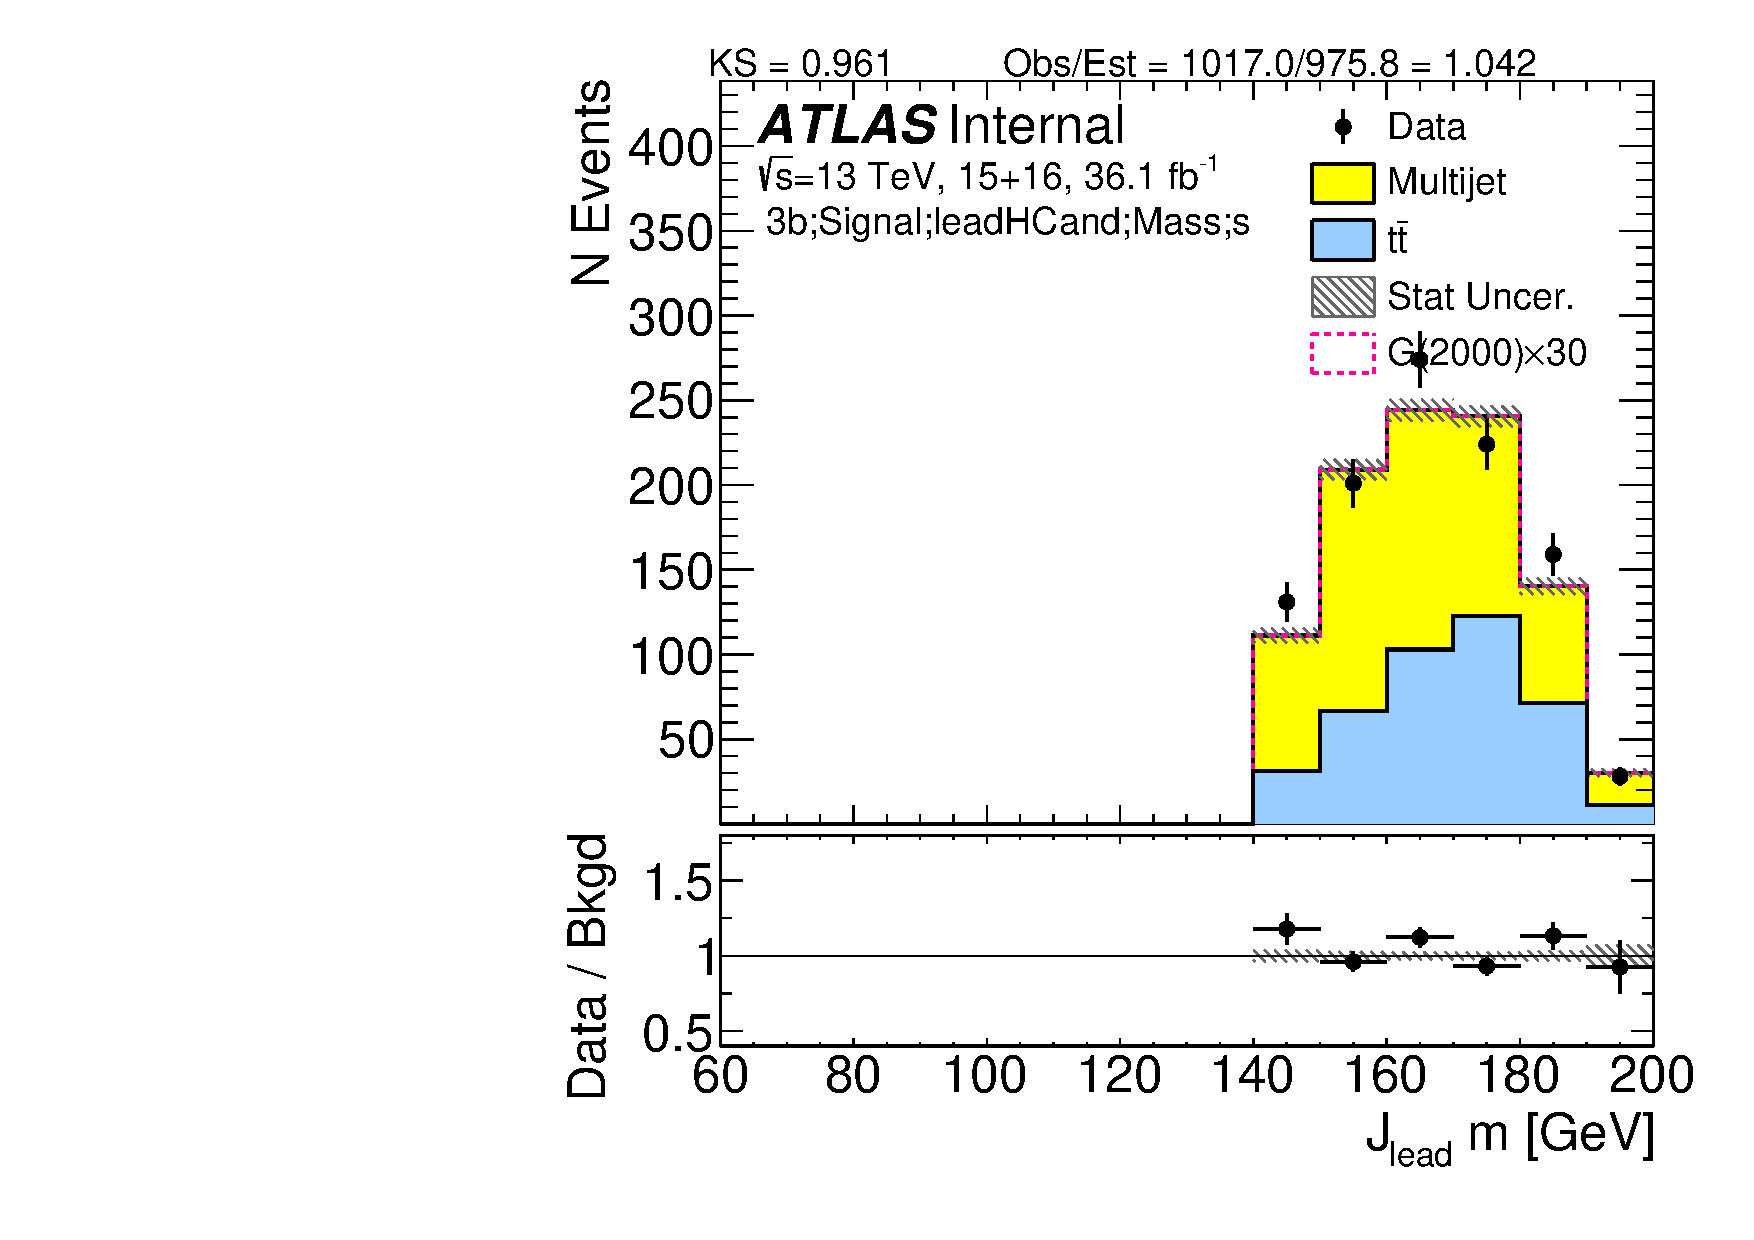
\includegraphics[width=0.45\textwidth,angle=-90]{figures/boosted/TT/Moriond_TT_ThreeTag_Signal_leadHCand_Mass_s.pdf}\\
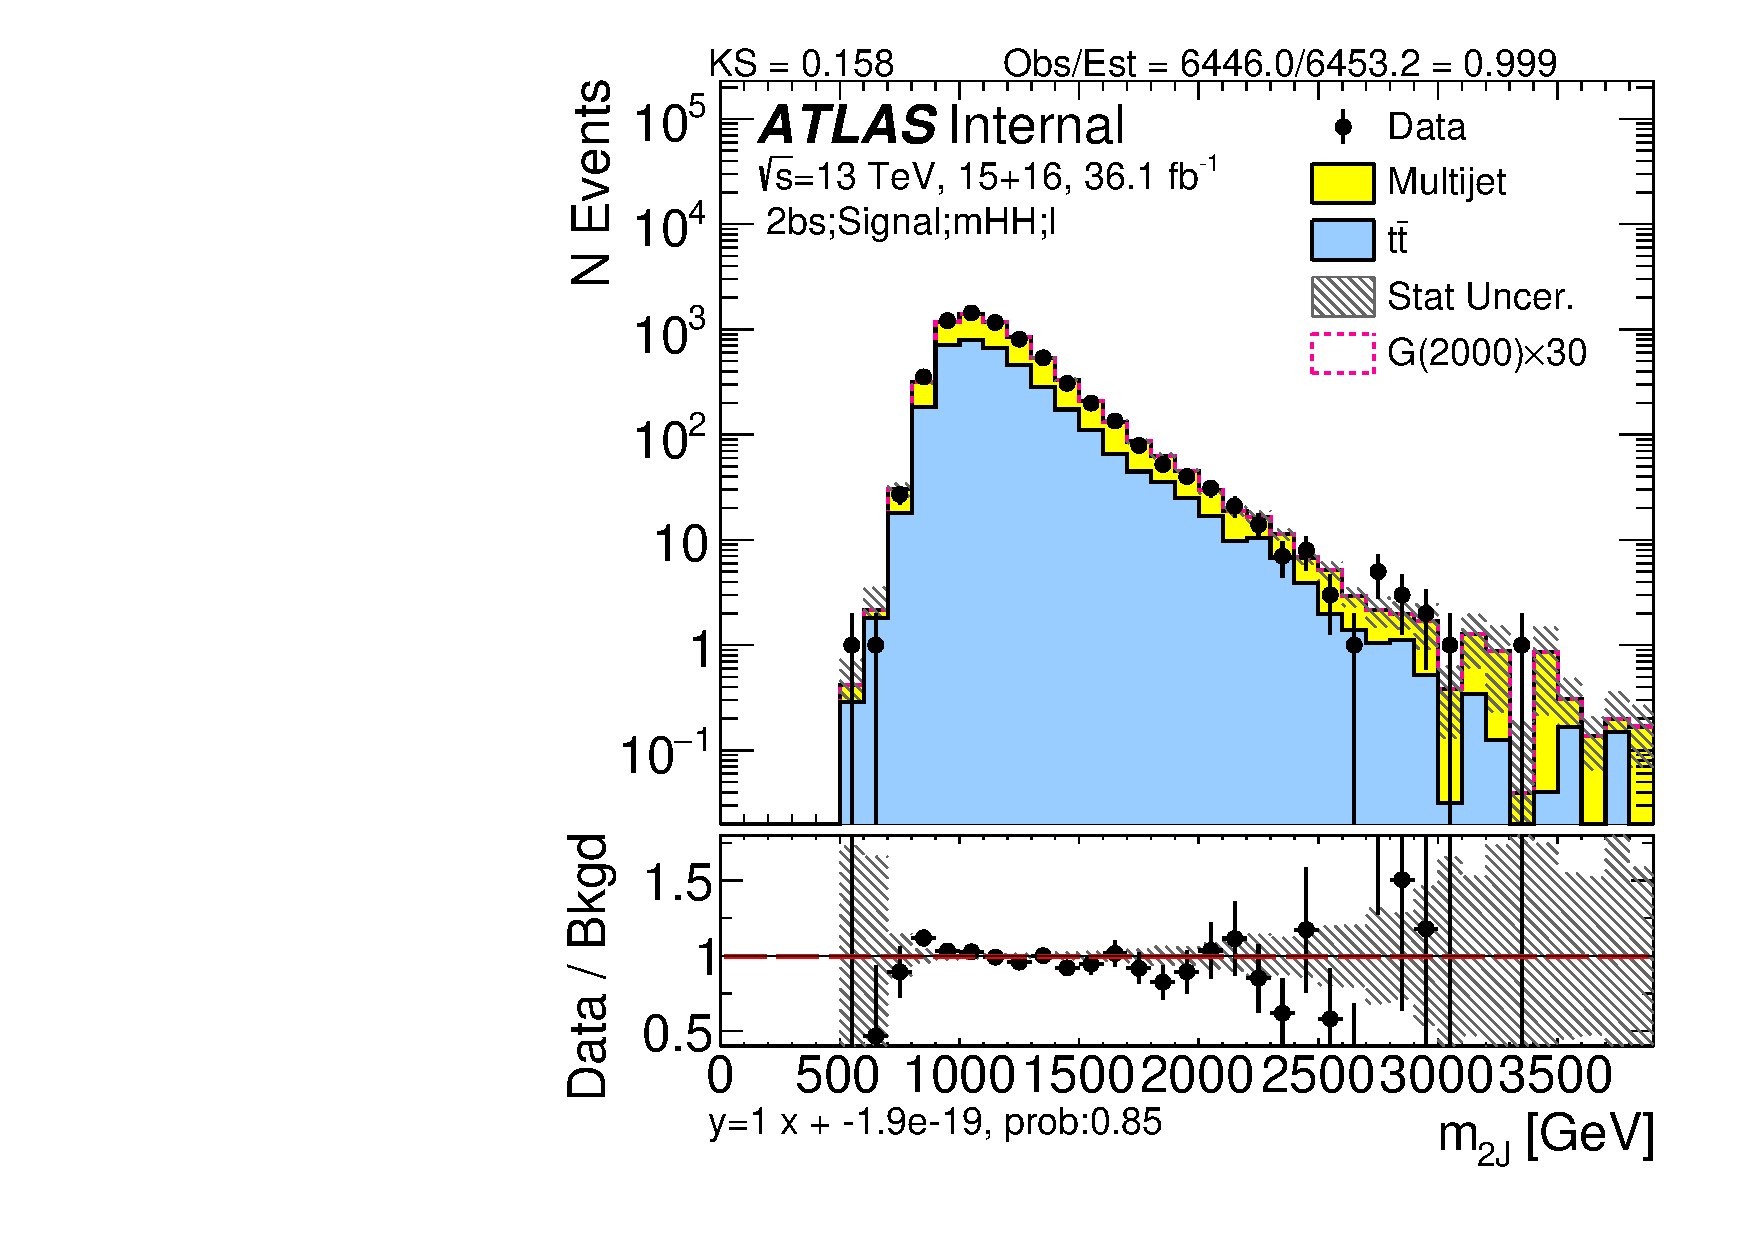
\includegraphics[width=0.45\textwidth,angle=-90]{figures/boosted/TT/Moriond_TT_TwoTag_split_Signal_mHH_l_1.pdf}
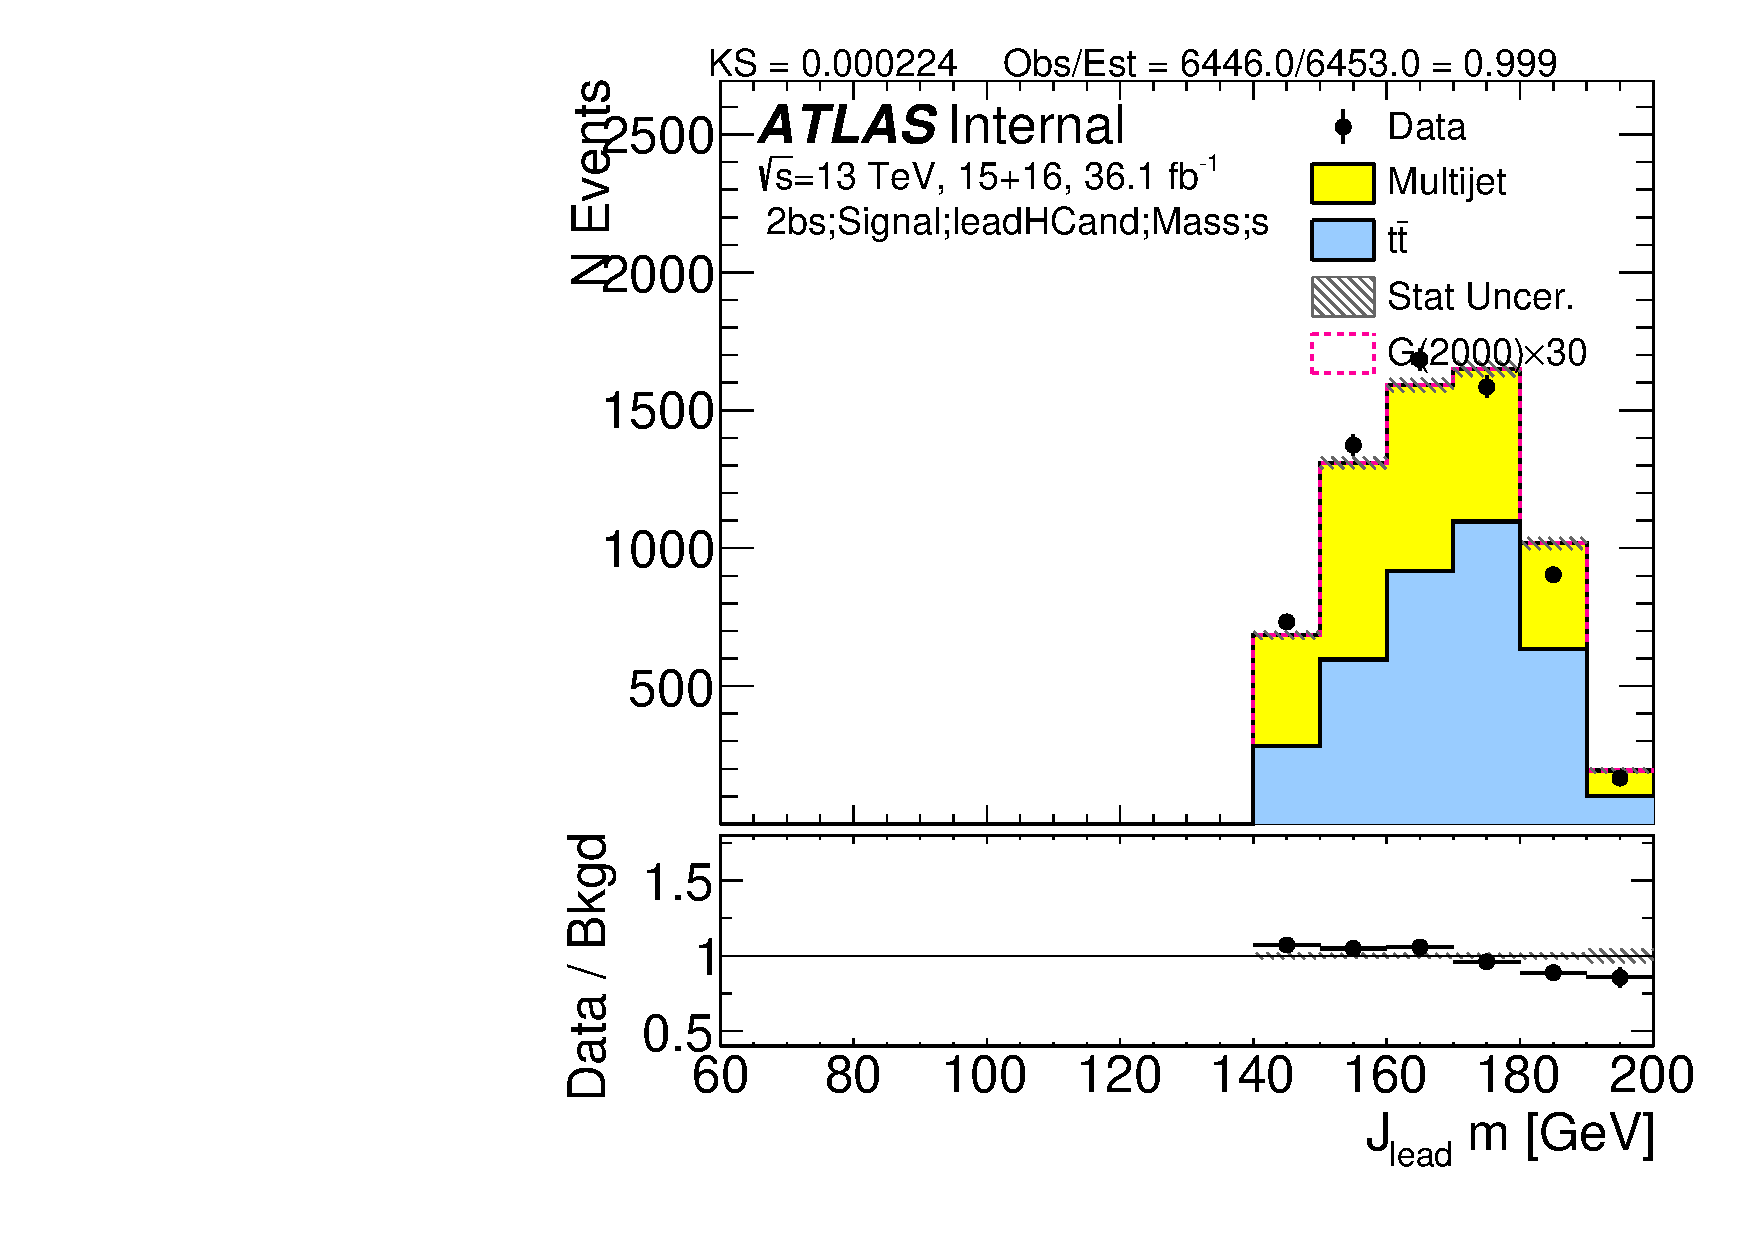
\includegraphics[width=0.45\textwidth,angle=-90]{figures/boosted/TT/Moriond_TT_TwoTag_split_Signal_leadHCand_Mass_s.pdf}\\
\end{center}
\caption{TT signal region distribution of di-jet mass (left column) and leading large-R jet mass (right column) in low mass signal, for $4b$ (top row), $3b$(middle row) and $2b$ split (bottom row). The plots are with only statistical uncertainty.}
\label{CRSB:TTSR_Distribution}
\end{figure}



\clearpage
\subsubsection{Uncertainty on the shape of the \ttbar\ jet mass in the $4/3b$ signal region}
\label{sec:unc-shape-ttbar-in-sr}

%In a similar method as stated in the previous section, the shape uncertainty of the signal region dijet mass in \ttbar\ events due to b-tagging or c-rejection is conservatively estimated by comparing the 0b, 1b, 2b, 3b, 4b distributions to the nominal 3b/4b shapes. Figure~\ref{ttbar-shapes-signal} shows the \ttbar\ leading jet and dijet mass distributions in the signal region, all normalized to the predicted number of events in the signal region from the simultaneous fit for \alphatt\ in the sideband.  
%All shapes are comparable within statistical uncertainties.  The difference in shape between the 2b and 3b distributions is taken as the \ttbar\ shape systematic in the signal region.  These shapes are further validated in data in a \ttbar-enriched region, as discussed in Section~\ref{sec:boosted-ttbar}.

\paragraph{}
Because the 4/3$b$ \ttbar\ MJJ distribution is extremely statistically limited, the 4/3$b$ shape is used to predict the final \ttbar\ background shape in the $2bs$ signal region. In order to estimate the possible shape uncertainty, the $2b$s and $3b$ sideband shapes are compared in Figure~\ref{fig:ttbar-shapes-signal} (after being normalized to the same area).  The $2b$s is used as there are not sufficient $4b$ statistics to asses the comparison quality. In order to avoid large statistical uncertainties, the distributions of the $3b$ and $2b$ are smoothed. The ratio of the two smoothed distributions is taken as the shape systematic. We then use this function to apply a bin-by-bin scaling of the \ttbar\ background prediction in the signal region, maintaining the same normalization given by nominal $t\bar{t}$ normalization prediction.

\begin{figure}[htbp!]
\begin{center} 
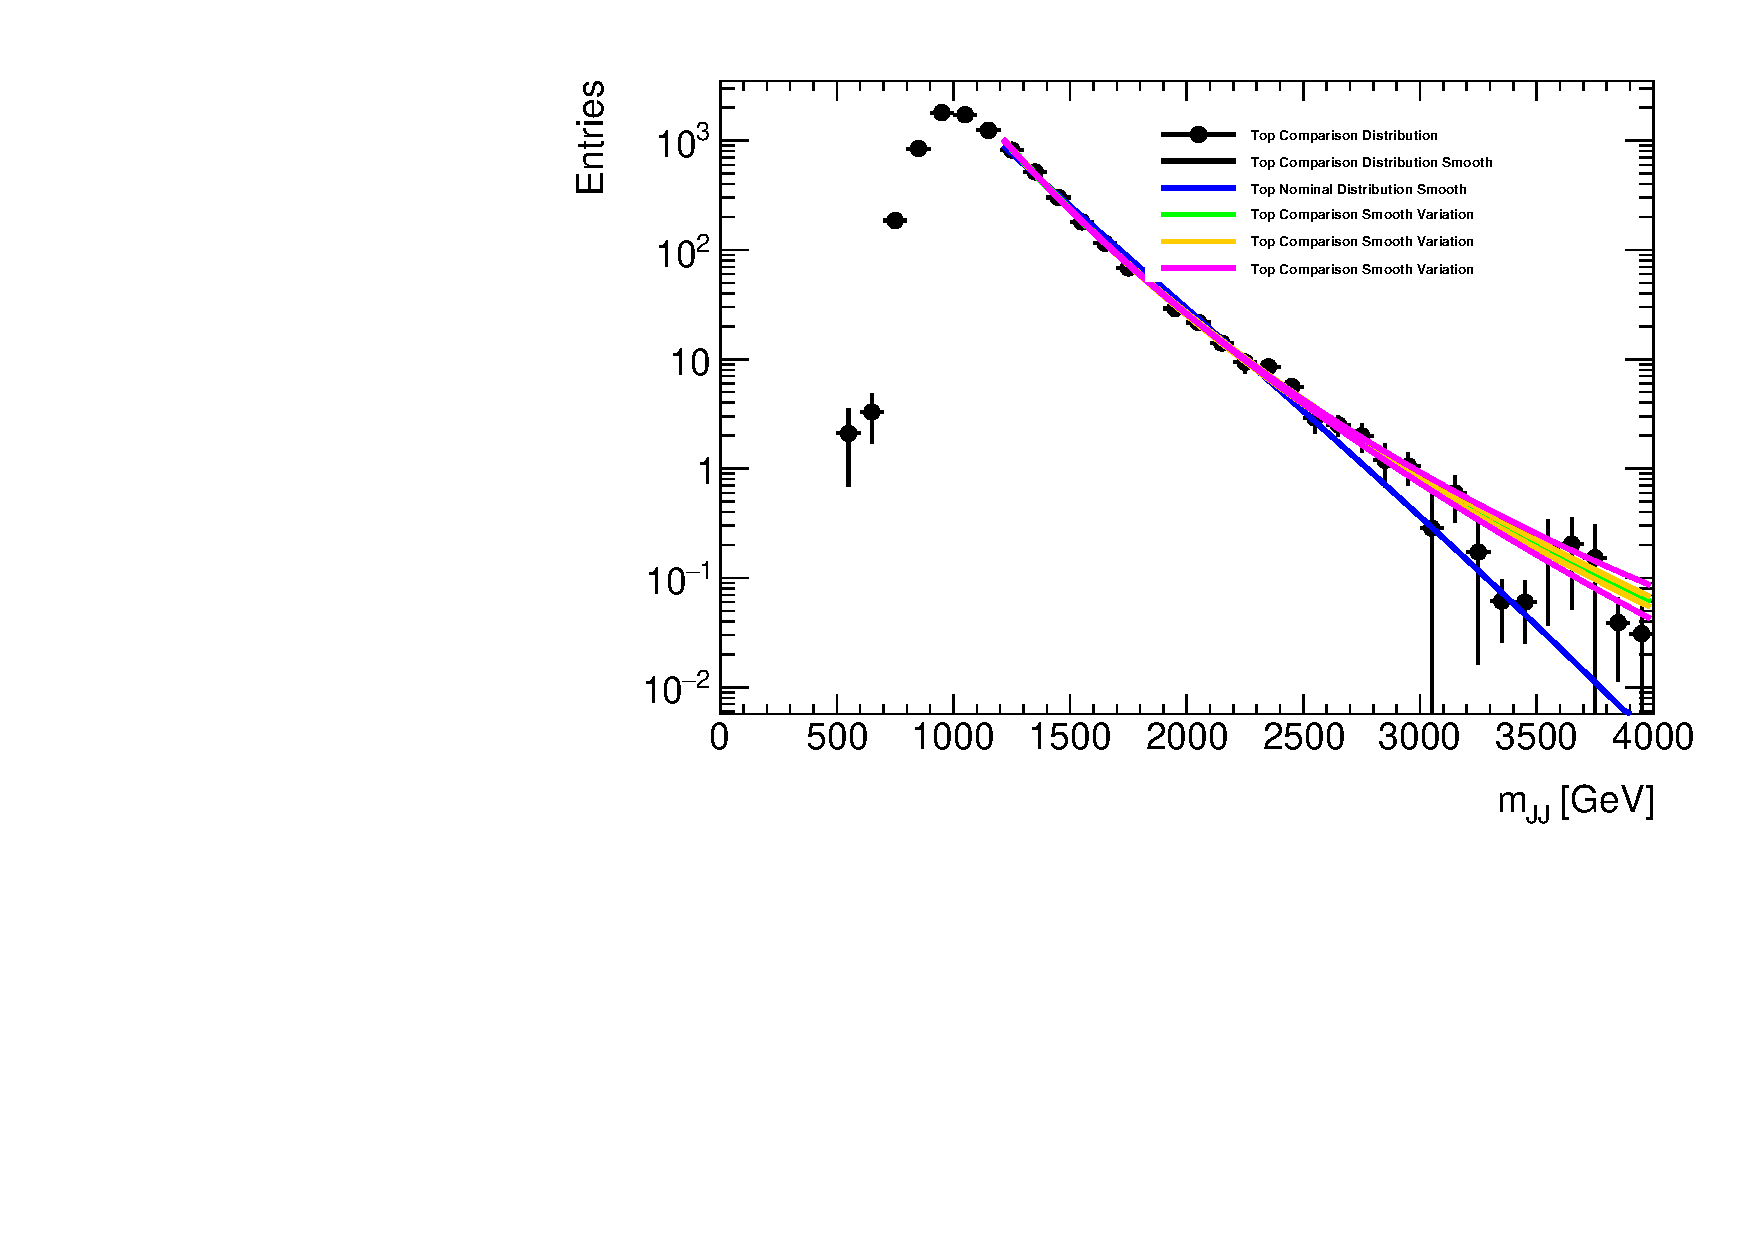
\includegraphics[angle=270, width=0.48\textwidth]{figures/boosted/Syst_Smooth/TopShapeSRSysfitSmooth_sig33_comp22.pdf}
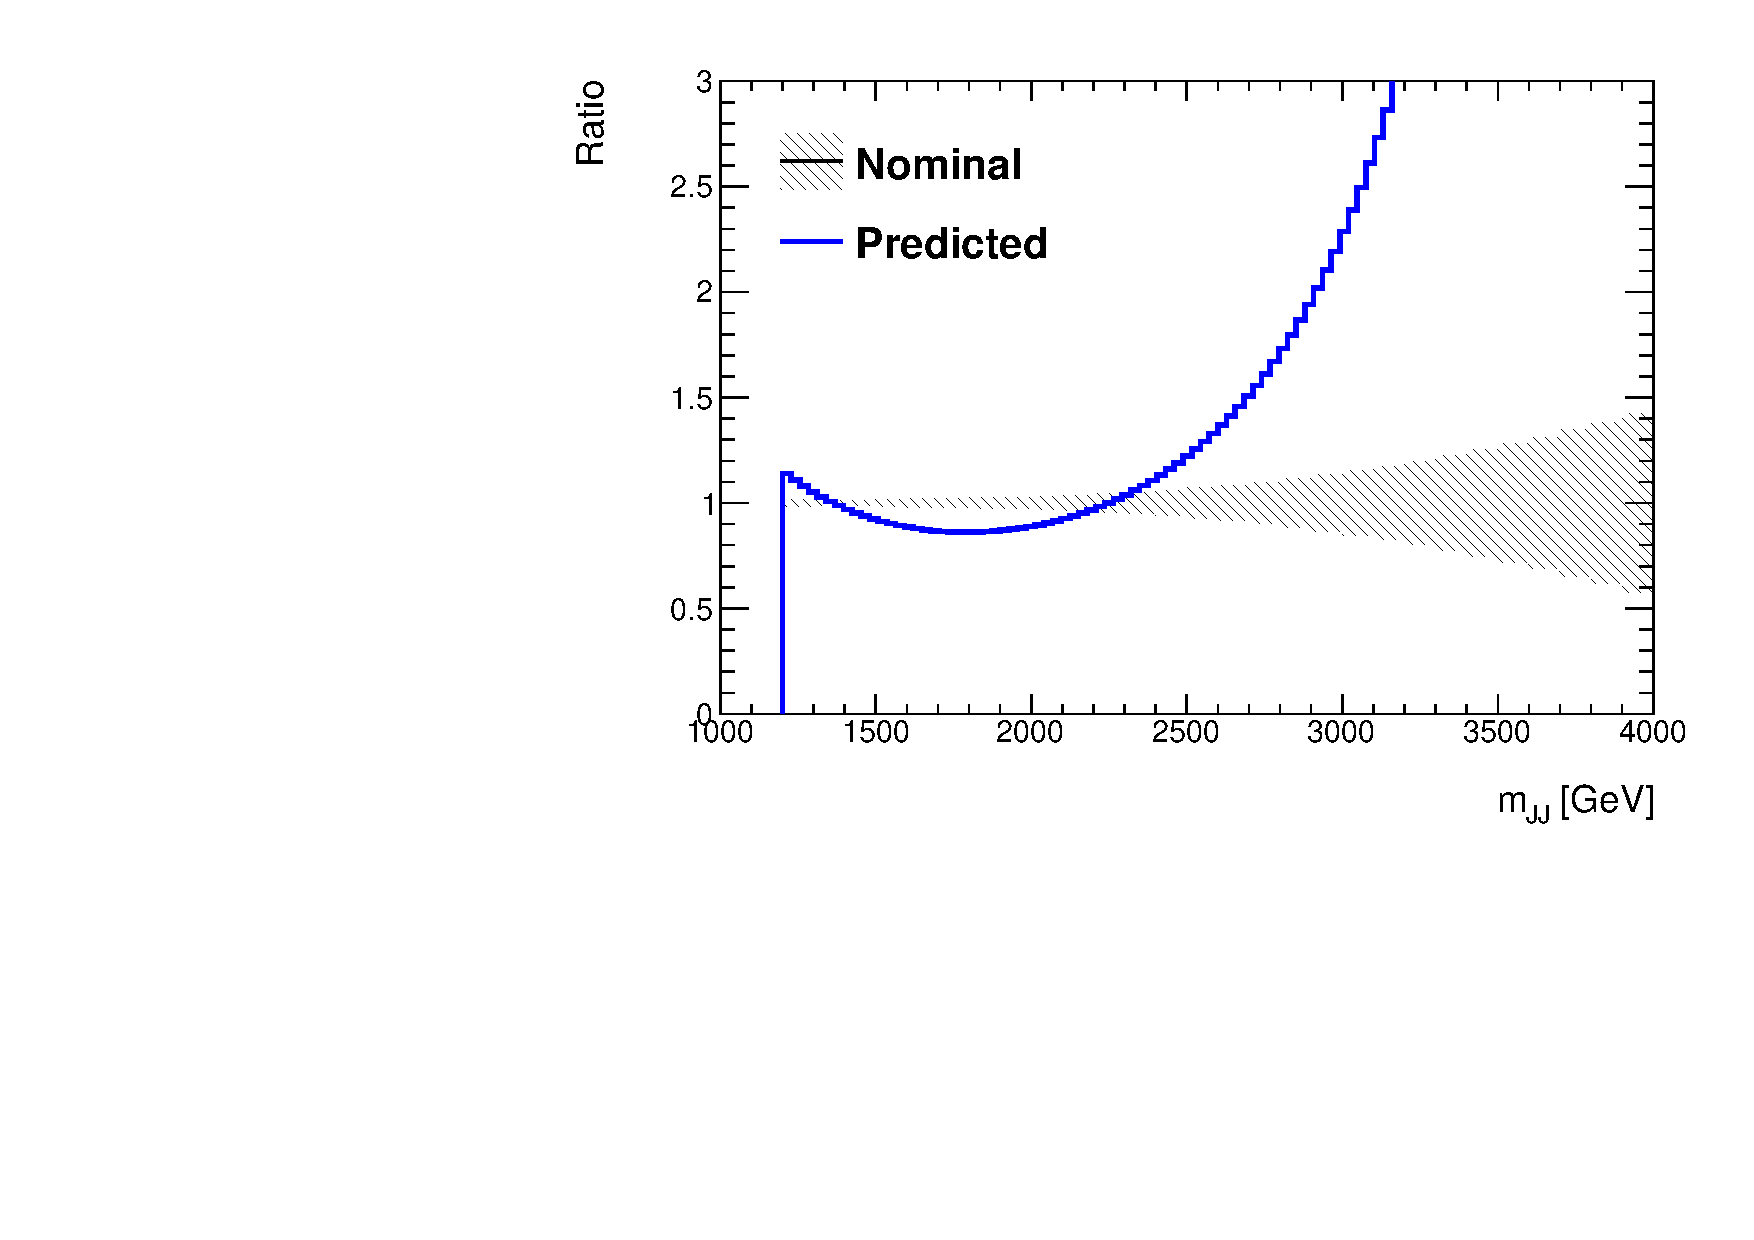
\includegraphics[angle=270, width=0.48\textwidth]{figures/boosted/Syst_Smooth/TopShapeSRSysfitSmooth_sig33_comp22_ratio.pdf}
\caption{(left)  Shape of the \ttbar\ di-\largeR-jet mass in the sideband region,
comparing the $3b$ shape with that of the $2b$, in order to asses the systematic effect of additional $b$-tags changing the dijet mass distribution.  The $m_{JJ}$ distributions is shown on the left, and the ratio of $3b$ to $2b$ distributions on the right.}
\label{fig:ttbar-shapes-signal}
\end{center}
\end{figure}

%The same method is applied to for the \ttbar\ shape uncertainty for the scaled dijet mass distribution.  The ratio of the $4b$ to $3b$ shape, as well as the linear fits and variations used to determine the shape uncertainty can be found in Figure~\ref{fig:ttbar-shapes-signal-scaled}.
%
%\begin{figure}[htbp!]
%\begin{center} 
%%%\includegraphics[angle=270, width=0.48\textwidth]{figures/boosted/background/DiJetMassPrime/topshape_44.pdf}
%\caption{The ratio of $4b$ to $3b$ shapes of the \ttbar\ scaled di-\largeR-jet mass in the signal region, with a linear fit to the ratio.  The same fit with negative slope is also shown on the figure.  \textbf{TO BE UPDATED} }
%\label{fig:ttbar-shapes-signal-scaled}
%\end{center}
%\end{figure}

\clearpage
\subsubsection{Uncertainty on the shape of the $1/2b$ QCD distribution in the signal region}
\label{unc-shape-qcd-in-sr}

\paragraph{}
As shown in Figures~\ref{fig:boosted-4b-control-ak10-system} and~\ref{fig:boosted-3b-control-ak10-system}, the shape distribution of the total predicted background using the scaled $1/2b$ QCD sample was found to be in good agreement with the 4$b$, 3$b$, and 2$b$s data in the control region.  However due to the low statistics in the data in the control region, the comparison is performed by first smoothing the $1/2b$, and the $4/3/2bs$ distributions. The ratio of the smoothed $1/2b$ distributions to that of the smoothed $4/3/2bs$ distributions is taken as the shape systematic. This function is then used to apply a bin-by-bin scaling of the QCD background prediction in the signal region, maintaining the same normalization given by \muqcd.  The CR distributions and the smoothing fit ratios can be found in Figure~\ref{fig:qcd_shape_fit}. This systematics is further split into two parts: one below 2000 \GeV and the other above 2000 \GeV, to ensure the low and high mass shape variation post-fit pulls can vary independently. It should be noted, that this uncertainty is used for both the dijet mass, and the scaled dijet mass distribution, and the correction to to scaling is expected to be small relative to the dijet mass. 

\begin{figure}[htbp!]
\begin{center}
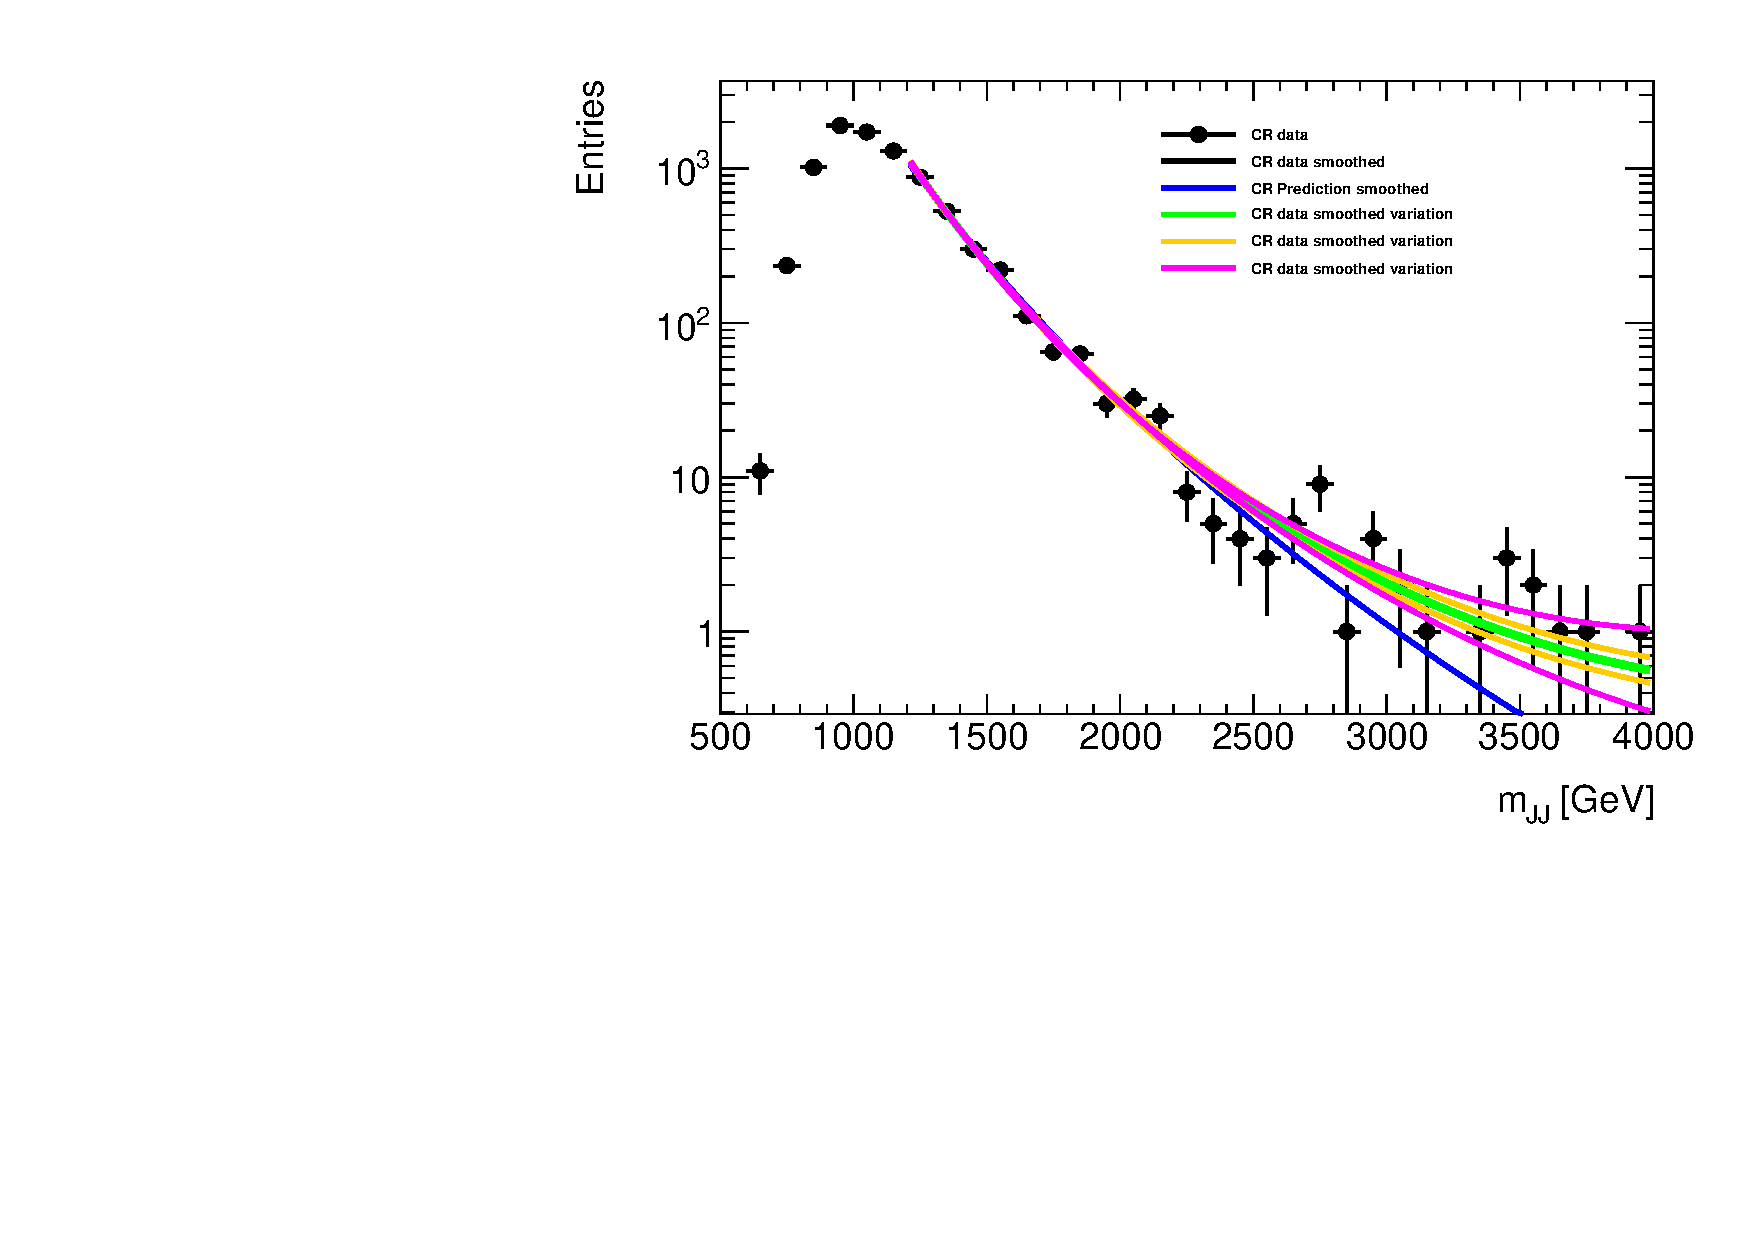
\includegraphics[angle=270, width=0.4\textwidth]{figures/boosted/Syst_Shape/QCDSysfitSmooth_22.pdf}
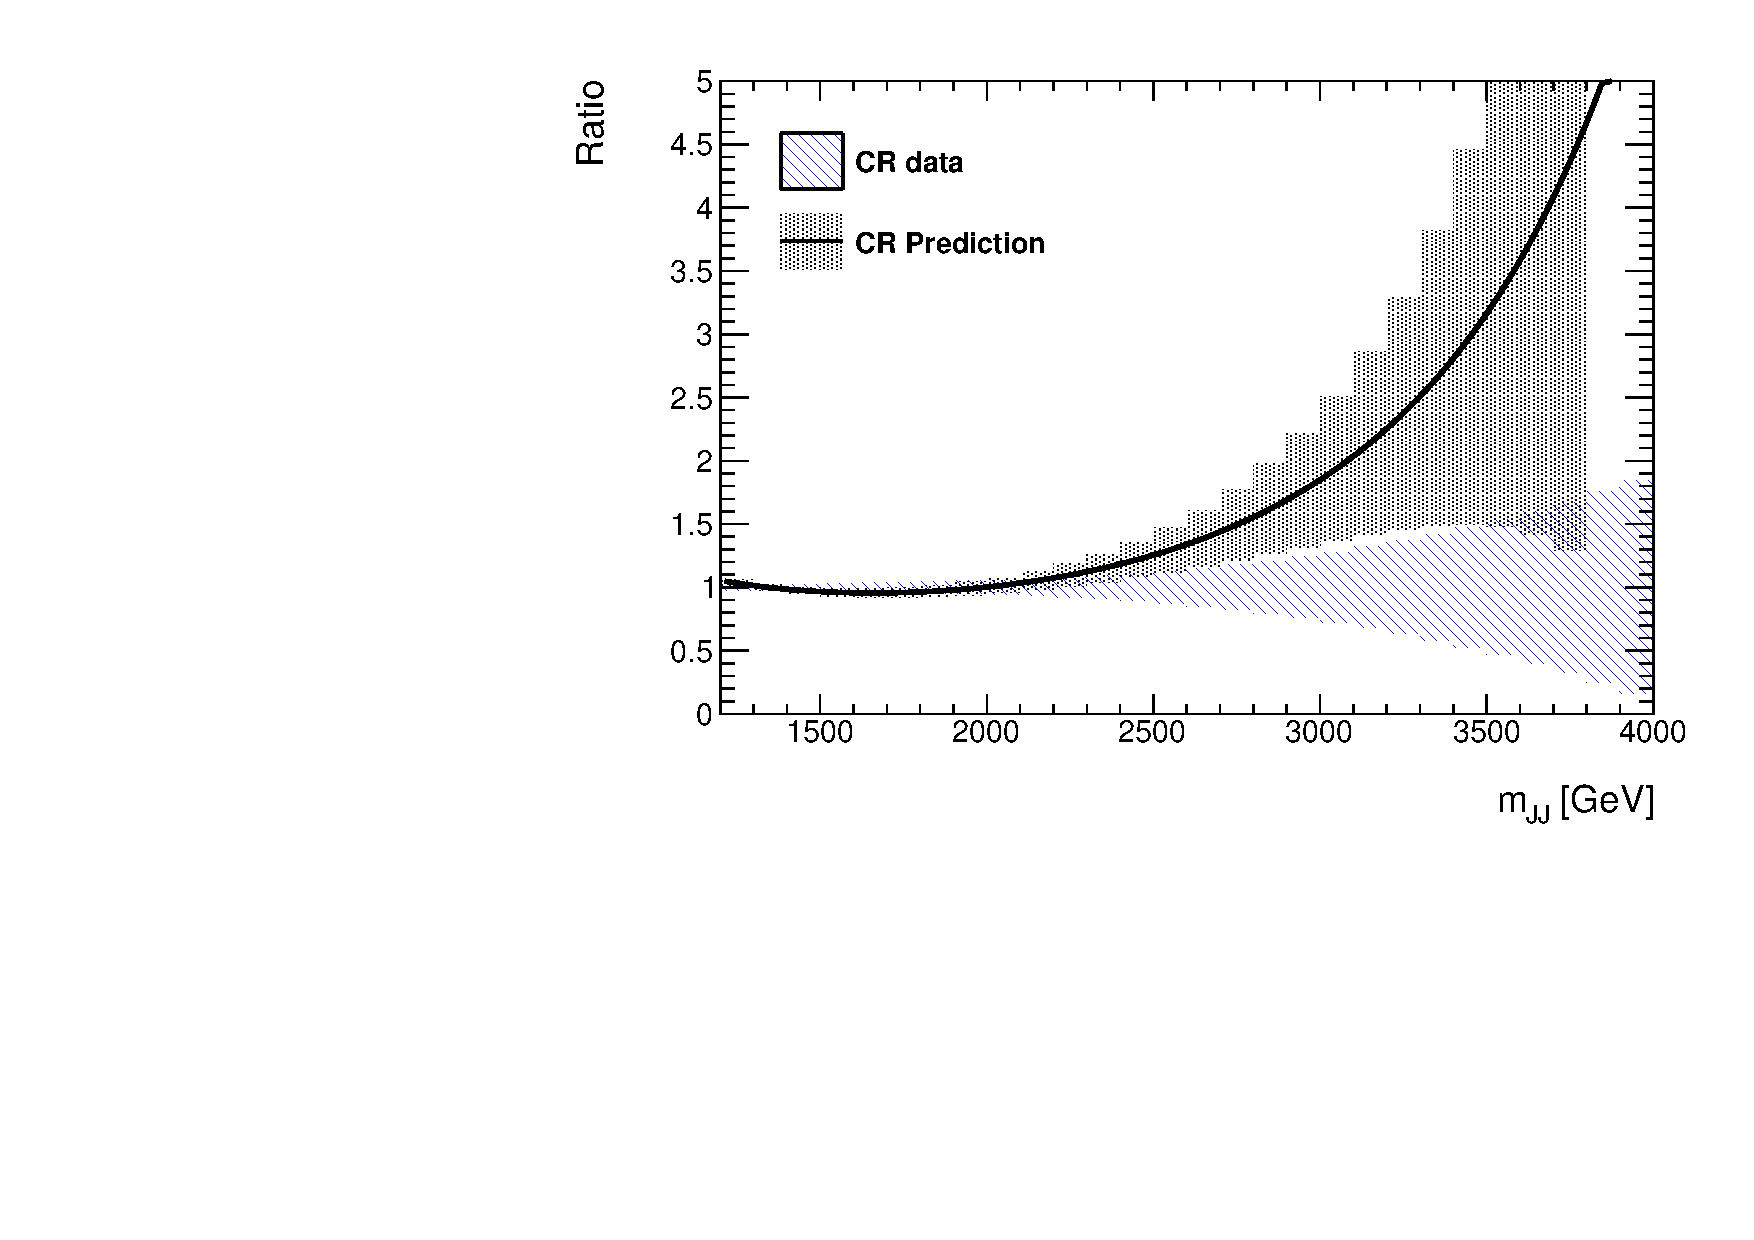
\includegraphics[angle=270, width=0.4\textwidth]{figures/boosted/Syst_Shape/QCDSysfitSmooth_ratio_22.pdf} \\
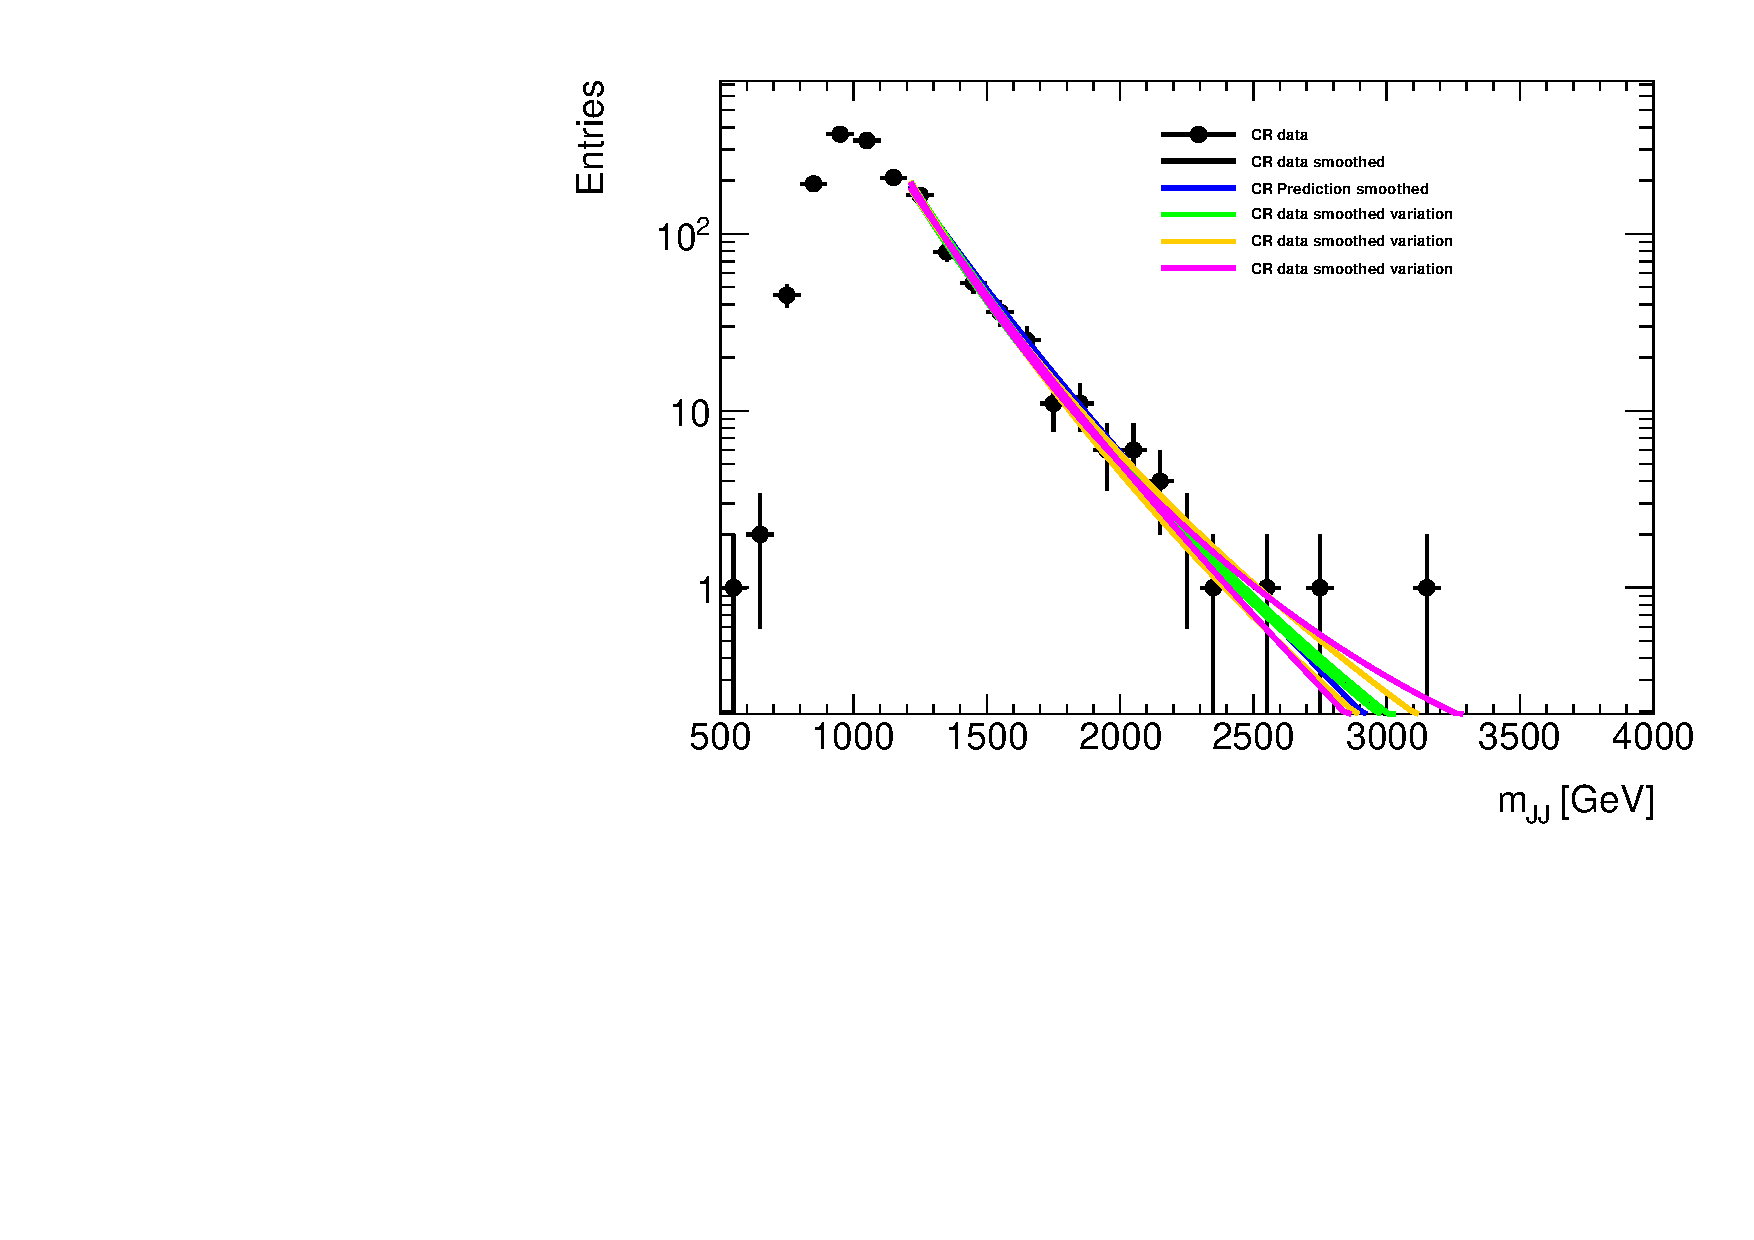
\includegraphics[angle=270, width=0.4\textwidth]{figures/boosted/Syst_Shape/QCDSysfitSmooth_33.pdf}
\includegraphics[angle=270, width=0.4\textwidth]{figures/boosted/Syst_Shape/QCDSysfitSmooth_ratio_33.pdf} \\
\includegraphics[angle=270, width=0.4\textwidth]{figures/boosted/Syst_Shape/QCDSysfitSmooth_44.pdf}
\includegraphics[angle=270, width=0.4\textwidth]{figures/boosted/Syst_Shape/QCDSysfitSmooth_ratio_44.pdf} \\
\caption{Dijet mass distribution in the CR along with the prediction (left) and the ratio of the prediction to the CR distribution (right)  for the 2$b$s (top) 3$b$ (middle) and 4$b$ (bottom) samples.  Ratios are from the smoothed distributions, the data uncertainty band contains the smoothing parameter variations, and the prediction uncertainty band also contains smoothing parameter variations.}
\label{fig:qcd_shape_fit}
\end{center}
\end{figure}

%\begin{figure}[htbp!]
%\begin{center}
%%%\includegraphics[angle=270, width=0.48\textwidth]{figures/boosted/systematics/QCDShapeSR/QCDShapeSR_44.pdf}
%%  %\includegraphics[angle=270, width=0.48\textwidth]{figures/boosted/systematics/QCDShapeSR/QCDShapeSR_43.pdf}
%\caption{Effect of the up/down variation of the 2b QCD shape in the $4b$ (left) and $3b$ (right) signal regions. Gray lines show the upwards and downwards variations.  \textbf{TO BE UPDATED} }
%\label{fig:qcd_shape_signal}
%\end{center}
%\end{figure}

%%\begin{figure}[ht!]
%%\begin{center}
%%  %%\includegraphics[angle=270, width=0.40\textwidth]{\figdir/systematics/QCD_shape/QCD_shape_scaled_signal.pdf}
%%  %%\includegraphics[angle=270, width=0.40\textwidth]{\figdir/systematics/QCD_shape/QCD_shape_scaled_signal_log.pdf}
%%\caption{Effect of the up/down variation of the 2b+3b QCD shape in the signal region with a linear y-axis scale (left) and a log scale (right).}
%%\label{fig:qcd_shape_control}
%%\end{center}
%%\end{figure}

\clearpage
\subsubsection{Uncertainty on QCD smoothing function in the signal region}
\label{unc-smooth-qcd-in-sr}

\paragraph{}
The MJ8 function has been used to fit the QCD background prediction in order to smooth the distribution and provide non-zero background estimates up to dijet masses beyond which we have $1/2b$ statistics.  While this distribution is  observed to fit the $1/2b$ data well, it does not have a concrete physical motivation, and in principle the high mass tail of the distribution could be larger than predicted by an exponential.  Two checks are performed, changing the boundaries where the fit is performed, and changing the fit function.

\paragraph{}
To test the impact of the region in which the fit is performed, we varied the upper bound on the dijet fit region to be each of the values $\{2800,\ 3000,\ 3200\}$ GeV and the starting value between $\{1200,\ 1300,\ 1400\}$ GeV.  The ratio of the fits for each upper bound, to that of the nominal (1200-3000 GeV) can be found in Figure~\ref{fig:qcd_fit_range_sys_ratio-scaled}, along with a hash band showing the statistical uncertainty of the nominal fit.  The maximum deviation from the nominal fit, per bin, is taken as the shape systematic uncertainy.  This is estimated separately for 2$b$s, 3$b$, and 4$b$ samples.

\paragraph{}
It should be noted that fits in which the fit $\chi^2$ probability was less than 0.001\%, or in which the fit integrals between 1500-2000 GeV, 2000-2500 GeV, or $>$2500 GeV were not in agreement with the original $1/2b$ distribution within a factor of 2 or 0.5, were not used to estimate the uncertainty.  The aforementioned checks ensure that we do not use poor fits of the $1/2b$ distribution to estimate the uncertainty.

%As we can see, changing the fit upper bound does not change the high mass tail prediction by large amounts, and is well within the statistical uncertainty of the nominal fit.  As a result, no additional systematic uncertainty is assigned for this fit range variation.

%\begin{figure}[htbp!]
%\begin{center}
%%%\includegraphics[angle=270, width=0.48\textwidth]{figures/boosted/systematics/QCDFitFunc/QCDFitFuncSys_range_ratio_44.pdf}
%% %\includegraphics[angle=270, width=0.48\textwidth]{figures/boosted/systematics/QCDFitFunc/QCDFitFuncSys_range_ratio_43.pdf}
%\caption{The ratio of the nominal exponential QCD prediction of the dijet mass distribution(with hashed band statistical uncertainties) to the predictions when fit with different upper bounds, in the $4b$ (left) and $3b$ (right) signal regions.  \textbf{TO BE UPDATED} }
%\label{fig:qcd_fit_range_sys_ratio}
%\end{center}
%\end{figure}

%The same test of changing the fit range for the scaled dijet mass distribution in the $4b$ and $3b$ signal regions has been performed, and the ratio of the different fit functions can be found in Figure~\ref{fig:qcd_fit_range_sys_ratio-scaled}.

\begin{figure}[htbp!]
\begin{center}
\includegraphics[angle=270, width=0.48\textwidth]{figures/boosted/Syst_Smooth/smoothFuncRangeCompare_22_comp.pdf}
\includegraphics[angle=270, width=0.48\textwidth]{figures/boosted/Syst_Smooth/smoothFuncRangeCompare_22_comp_ratio.pdf} \\
\includegraphics[angle=270, width=0.48\textwidth]{figures/boosted/Syst_Smooth/smoothFuncRangeCompare_33_comp.pdf}
\includegraphics[angle=270, width=0.48\textwidth]{figures/boosted/Syst_Smooth/smoothFuncRangeCompare_33_comp_ratio.pdf} \\
\includegraphics[angle=270, width=0.48\textwidth]{figures/boosted/Syst_Smooth/smoothFuncRangeCompare_44_comp.pdf}
\includegraphics[angle=270, width=0.48\textwidth]{figures/boosted/Syst_Smooth/smoothFuncRangeCompare_44_comp_ratio.pdf} \\
\caption{Dijet mass distribution SR prediction fit with several fit ranges (left) and the ratio of nominal to fits with different fit ranges (right)  for the 2b (top) 3b (middle) and 4b (bottom) samples. }
\label{fig:qcd_fit_range_sys_ratio-scaled}
\end{center}
\end{figure}

\paragraph{}
As a second test, we fit the $1/2b$ QCD prediction with a variety of other distributions which can show both power law behavior in the bulk of the distribution as well as longer tails.  The set of additional functions examined (labelled MJ1-MJ7) can be found in Table~\ref{tab:fit_funcs}, where $x = m_{JJ} / \sqrt{s}$.

\begin{table}[htbp!]
\begin{center} 
\begin{tabular}{  l | c}
%\footnotesize
Name & Functional Form \\
\hline
MJ1 (Dijet) & $f_{1}(x) = p_0 (1-x)^{p_1} x^{p_2}$ \\
MJ2 & $f_{2}(x) = p_0 (1-x)^{p_1} e^{p_2\ x^2}$ \\
MJ3 & $f_{3}(x) = p_0 (1-x)^{p_1} x^{p_2\ x}$ \\
MJ4 & $f_{4}(x) = p_0 (1-x)^{p_1} x^{p_2\ ln\ x}$ \\
MJ5 & $f_{5}(x) = p_0 (1-x)^{p_1} (1+x)^{p_2\ x}$ \\
MJ6 & $f_{6}(x) = p_0 (1-x)^{p_1} (1+x)^{p_2\ ln\ x}$ \\
MJ7 & $f_{7}(x) = \frac{p_0}{x} (1-x)^{p_1 - p_2\ ln\ x}$ \\
MJ8 & $f_{8}(x) = \frac{p_0}{x^2} (1-x)^{p_1 - p_2\ ln\ x}$ \\
\hline
\end{tabular}
\caption{Functions used to fit the QCD dijet mass distributions, where $x = m_{JJ} / \sqrt{s}$.}
\label{tab:fit_funcs}
\end{center}
\end{table}

\paragraph{}
Figure~\ref{fig:qcd_fit_funcs_sys} shows the fits to the QCD prediction in the 4/3/2b  signal regions, and the nominal dijet fit, as well as the ratios of the nominal fit to that of the additional functions.  The maximum per bin deviation is taken as the shape systematic, separately for the 4/3/2b SRs.

\paragraph{}
As before, fits in which the fit $\chi^2$ probability was less than 0.1\%,  or in which the fit integrals between 1500-2000 GeV, 2000-2500 GeV, or $>$2500 GeV were not in agreement with the original 0b distribution within a factor of 2 or 0.5, were not used to estimate the uncertainty.  The aforementioned checks ensure that we do not use poor fits of the 0b distribution to estimate the uncertainty.

\begin{figure}[htbp!]
\begin{center}
\includegraphics[angle=270, width=0.48\textwidth]{figures/boosted/Syst_Smooth/smoothFuncCompare_22_comp.pdf}
\includegraphics[angle=270, width=0.48\textwidth]{figures/boosted/Syst_Smooth/smoothFuncCompare_22_comp_ratio.pdf} \\
\includegraphics[angle=270, width=0.48\textwidth]{figures/boosted/Syst_Smooth/smoothFuncCompare_33_comp.pdf}
\includegraphics[angle=270, width=0.48\textwidth]{figures/boosted/Syst_Smooth/smoothFuncCompare_33_comp_ratio.pdf} \\
\includegraphics[angle=270, width=0.48\textwidth]{figures/boosted/Syst_Smooth/smoothFuncCompare_44_comp.pdf}
\includegraphics[angle=270, width=0.48\textwidth]{figures/boosted/Syst_Smooth/smoothFuncCompare_44_comp_ratio.pdf} \\
\caption{ Dijet mass distribution SR prediction fit with several fit functions (left) and the ratio of nominal to fits with different fit functions (right)  for the 2b (top) 3b (middle) and 4b (bottom) samples. The additional fit functions are from Table~\ref{tab:fit_funcs}.}
\label{fig:qcd_fit_funcs_sys}
\end{center}
\end{figure}

%%%
%%%In addition, we examined the consistency between all the variations of the fit parameters from all of the additional function, with the nominal exponential.  The ratio of predictions can be found in Figure~\ref{fig:qcd_fit_funcs_sys_super_ratio}, where the gray lines are the parameter variations from all the additional functions.  Most of these variations are contained in the hashed band, representing the statistical uncertainty of the nominal exponential fit.
%%%
%%%\begin{figure}[htbp!]
%%%\begin{center}
%%%%%\includegraphics[angle=270, width=0.48\textwidth]{figures/boosted/systematics/QCDFitFunc/QCDFitFuncSys_ratio_super_44.pdf}
%%%% %\includegraphics[angle=270, width=0.48\textwidth]{figures/boosted/systematics/QCDFitFunc/QCDFitFuncSys_ratio_super_43.pdf}
%%%\caption{The ratio of the nominal exponential QCD prediction of the dijet mass distribution (with hashed band statistical uncertainties) to the predictions of the additional fit functions of Table~\ref{tab:fit_funcs} in the $4b$ (left) and $3b$ (right) signal regions.  \textbf{TO BE UPDATED} }
%%%\label{fig:qcd_fit_funcs_sys_super_ratio}
%%%\end{center}
%%%\end{figure}
%%%
%%%
%%%
%%%As a conservative systematic, the bin-by-bin largest difference between the exponential prediction and the set of additional fit functions or any of the additional function parameter variations is taken as the fit function uncertainty.
%%%
%%%To validate this uncertainty, we perform smoothing on the dijet mass distributions in the CR, and compute the smoothing uncertainties as described above.  The comparison with the CR data can be seen in Figure~\ref{fig:qcd_fit_funcs_sys_check_CR}, where the prediction includes all uncertainties (including the smoothing uncertainty) except the CR shape and normalization uncertainty which was derived from this distribution.  We can see that within uncertainties, the predictions is in good agreement with the CR data.
%%%
%%%\begin{figure}[htbp!]
%%%\begin{center}
%%%%%\includegraphics[angle=270, width=0.48\textwidth]{figures/boosted/background/DrawCompleteBkgEst_DiJetMass_Pass4GoodTrackJetPass4b77PassCRMass_smoothed.pdf}
%%%% %\includegraphics[angle=270, width=0.48\textwidth]{figures/boosted/background/DrawCompleteBkgEst_DiJetMass_Pass4GoodTrackJetPass3b77PassCRMass_smoothed.pdf}
%%%\caption{Smoothing prediction applied in the CR compared with data in the $4b$ (left) and $3b$ (right) signal regions. Hashed band show all uncertainties, including the smoothing uncertainties,  except the CR shape and normalization uncertainty which was derived from this distribution.  \textbf{TO BE UPDATED} }
%%%\label{fig:qcd_fit_funcs_sys_check_CR}
%%%\end{center}
%%%\end{figure}
%%%
%%%
%%%
%%%
%%%
%%%The additional smoothing functions are also tested in the case of using the scaled dijet mass distribution, as seen in Figure~\ref{fig:qcd_fit_funcs_sys-scaled}, and the ratio to the nominal fit can be found in Figure~\ref{fig:qcd_fit_funcs_sys_ratio-scaled}, for the $4b$ and $3b$ signal regions.  The same distributions, including also all variations of the parameters of the additional functions within statistical uncertainty, is shown in Figure~\ref{fig:qcd_fit_funcs_sys_super-scaled} and Figure~\ref{fig:qcd_fit_funcs_sys_super_ratio-scaled}.  To be conservative, the maximum bin-by-bin difference between the nominal exponential fit, and any of the variations of the additional functions, is taken as the extrapolation uncertainty.
%%%
%%%
%%%\begin{figure}[htbp!]
%%%\begin{center}
%%%%%\includegraphics[angle=270, width=0.48\textwidth]{figures/boosted/background/DiJetMassPrime/qcd_smoothfit_FuncComp_44.pdf}
%%%% %\includegraphics[angle=270, width=0.48\textwidth]{figures/boosted/background/DiJetMassPrime/qcd_smoothfit_FuncComp_43.pdf}
%%%\caption{The QCD prediction of the scaled dijet mass distribution in the $4b$ (left) and $3b$ (right) signal regions, showing the nominal exponential fit (with has band statistical uncertainties) and the additional fits from Table~\ref{tab:fit_funcs}. \textbf{TO BE UPDATED} }
%%%\label{fig:qcd_fit_funcs_sys-scaled}
%%%\end{center}
%%%\end{figure}
%%%
%%%\begin{figure}[htbp!]
%%%\begin{center}
%%%%%\includegraphics[angle=270, width=0.48\textwidth]{figures/boosted/background/DiJetMassPrime/smoothfunc_ratio_44.pdf}
%%%% %\includegraphics[angle=270, width=0.48\textwidth]{figures/boosted/background/DiJetMassPrime/smoothfunc_ratio_43.pdf}
%%%\caption{The ratio of the nominal exponential QCD prediction of the scaled dijet mass distribution (with hashed band statistical uncertainties) to the predictions of the additional fit functions of Table~\ref{tab:fit_funcs} in the $4b$ (left) and $3b$ (right) signal regions.  \textbf{TO BE UPDATED} }
%%%\label{fig:qcd_fit_funcs_sys_ratio-scaled}
%%%\end{center}
%%%\end{figure}
%%%
%%%\begin{figure}[htbp!]
%%%\begin{center}
%%%%%\includegraphics[angle=270, width=0.48\textwidth]{figures/boosted/background/DiJetMassPrime/qcd_smoothfit_FuncCompSuper_44.pdf}
%%%% %\includegraphics[angle=270, width=0.48\textwidth]{figures/boosted/background/DiJetMassPrime/qcd_smoothfit_FuncCompSuper_43.pdf}
%%%\caption{The QCD prediction of the scaled dijet mass distribution in the $4b$ (left) and $3b$ (right) signal regions, showing the nominal exponential fit (with has band statistical uncertainties) and the additional fits from Table~\ref{tab:fit_funcs}.  \textbf{TO BE UPDATED} }
%%%\label{fig:qcd_fit_funcs_sys_super-scaled}
%%%\end{center}
%%%\end{figure}
%%%
%%%\begin{figure}[htbp!]
%%%\begin{center}
%%%%%\includegraphics[angle=270, width=0.48\textwidth]{figures/boosted/background/DiJetMassPrime/smoothfunc_ratio_44_extrap.pdf}
%%%% %\includegraphics[angle=270, width=0.48\textwidth]{figures/boosted/background/DiJetMassPrime/smoothfunc_ratio_43_extrap.pdf}
%%%\caption{The ratio of the nominal exponential QCD prediction of the scaled dijet mass distribution (with hashed band statistical uncertainties) to the predictions of the additional fit functions of Table~\ref{tab:fit_funcs} in the $4b$ (left) and $3b$ (right) signal regions, including all parameter variations of the additional functions.  \textbf{TO BE UPDATED} }
%%%\label{fig:qcd_fit_funcs_sys_super_ratio-scaled}
%%%\end{center}
%%%\end{figure}

\clearpage
%\paragraph{Tests of $\mu_{QCD}$ extrapolation}
%\label{sec:boosted-extrapolation}
%\hspace{0.1mm}\newline
%%\input{Sections/sec-boosted-extrapolations}



\subsection{Summary of systematics}
\label{sec:boosted-systematics-numbers}
%%\paragraph{}
Table~\ref{tab:summary-systematics-4b} shows the percent impact of systematics used in this analysis on the backgrounds yields and on the expected yields for RSG $c=1.0$ signals in the $4b$ signal region. The correspondent values are shown for the $3b$ signal region in Table ~\ref{tab:summary-systematics-3b}, and are shown for the $2bs$ signal region in Table ~\ref{tab:summary-systematics-2b}. 

%%\paragraph{}
A 3.2\% luminosity uncertainty is also considered for the Z+jets background and the RSG signal predictions. The JER/JMR/JES/JMS/track jet b-tag scale factor uncertainties are applied to RSG and \ttbar\ samples. 

%%\paragraph{}
The ``\ttbar\ SB shape'' is the background normalization uncertainty due to the mis-modeling of the 
shape of the \ttbar\ dijet mass distribution in the sideband region, taken from comparing the shape with 3/4 $b$-tags to the shape with only a 2bs requirement. The ``Background Normalization Fit'' uncertainty comes from summing in quadrature the independent uncertainty components calculated from the correlated statistical errors of \muqcd and \alphatt  The ``QCD Non-Closure in CR'' systematic is derived as the maximum of (a) difference between the predicted and observed 4b/3b/2bs QCD yields in the control region, (b) the fractional change in SR predictions from varying the CR and SB definitions.  Both options gave similar sized uncertainties, but the uncertainty from the CR/SB variations was found to be larger. All these uncertainties are summed in quarature and shown in the ``Bkg Est'' row in the table.

%%\paragraph{}
The remaining systematics not listed in this table, as they do not impact the acceptance, include uncertainties on the shape of the QCD and \ttbar\ backgrounds in the signal region, and the uncertainties from the smoothing / extrapolation procedure.

%%\paragraph{}
The size of the Monte Carlo modeling systematics on the RSG c=1.0 signal yield as a function of the signal mass can be found in Figure~\ref{fig:signal_syst_summary}. These uncertainties have a similar impact on the other signals. The largest uncertainty in the $4b$ and $2b$ signal region is from $b$-tagging, followed by the JMR uncertainty. In the $3b$ signal region, although $b$-tagging systematics is still one of the largest uncertainty, it has been much reduced compared to $4b$ region, as discussed in Section~\ref{sec:b-tagging-unc}. Then the jet mass scale and resolution are the largest uncertainties following b-tagging. 

%%%\paragraph{}
%\textbf{It should be noted that as numbers in this version of the note, the \ttbar\ MC systematics are reduced, because of the larger stat $2bs$ \ttbar to model $3b$ and $4b$ \ttbar shape estimation. This is applied for JER, JMR, and \ttbar MC generator variations.}

\begin{table}[htbp!]
\scriptsize
\begin{center}
\begin{footnotesize} 
\begin{tabular}{c|c|c|c|c|c|c} 
FourTag & totalbkg & qcd & ttbar & RSG1 1000 & RSG1 2000 & RSG1 3000 \\ 
\hline\hline 
JER & 0.45 & 0.27 & 3.98 & 2.44 & 1.07 & 0.67\\ 
JMR & 7.9 & 10.35 & 39.95 & 12.33 & 13.16 & 15.08\\ 
Top &  -  &  -  &  -  &  -  &  -  &  - \\ 
JES/JMS & 1.32 & 1.49 & 24.36 & 5.18 & 3.72 & 5.62\\ 
Bkg Est & 15.67 & 18.19 & 67.82 &  -  &  -  &  - \\ 
b-tag SF & 1.11 & 0.79 & 18.85 & 18.34 & 28.11 & 27.73\\ 
\hline 
Total Sys & 17.64 & 21.0 & 84.62 & 22.83 & 31.28 & 32.07\\ 
\hline 
Stat & 3.13 & 3.29 & 2.47 & 1.97 & 1.63 & 4.9\\ 
\hline 
Estimated Events & 34.59 & 32.91 & 1.68 & 10.07 & 0.25 & 0.0016\\ 
\hline\hline 
\end{tabular} 
\end{footnotesize} 
\newline 

\caption{Percent impact of the dominant systematics on the  background acceptance
         and on the signal acceptance of RS $c=1.0$ graviton predictions in the $4b$ signal region.}
\label{tab:summary-systematics-4b}
\end{center}
\end{table}

% \begin{table}[htbp!]
% \scriptsize
% \begin{center}
% %\input{figures/tables/SystematicTable_44_OtherSignal.tex}
% \caption{Percent impact of the dominant systematics on the signal acceptance of RS $c=2.0$ graviton and 2HDM predictions in the $4b$ signal region. \textbf{TO BE UPDATED} }
% \label{tab:summary-systematics-4b-OtherSignal}
% \end{center}
% \end{table}

\begin{table}[htbp!]
\scriptsize
\begin{center}
\begin{footnotesize} 
\begin{tabular}{c|c|c|c|c|c|c} 
ThreeTag & totalbkg & qcd & ttbar & RSG1 1000 & RSG1 2000 & RSG1 3000 \\ 
\hline\hline 
JER & 1.38 & 3.52 & 17.5 & 1.41 & 0.93 & 1.08\\ 
JMR & 1.35 & 4.26 & 24.38 & 14.3 & 12.33 & 15.53\\ 
Top &  -  &  -  &  -  &  -  &  -  &  - \\ 
JES/JMS & 2.03 & 1.26 & 26.22 & 5.19 & 1.94 & 6.35\\ 
Bkg Est & 4.84 & 5.62 & 9.45 &  -  &  -  &  - \\ 
b-tag SF & 0.47 & 0.53 & 8.45 & 2.45 & 2.01 & 9.27\\ 
\hline 
Total Sys & 5.61 & 8.0 & 41.82 & 15.47 & 12.68 & 19.2\\ 
\hline 
Stat & 1.32 & 1.44 & 2.47 & 1.26 & 1.0 & 1.83\\ 
\hline 
Estimated Events & 780.89 & 701.52 & 79.38 & 26.0 & 0.76 & 0.013\\ 
\hline\hline 
\end{tabular} 
\end{footnotesize} 
\newline 

\caption{Percent impact of the dominant systematics on the  background acceptance
         and on the signal acceptance of RS $c=1.0$ graviton predictions in the $3b$ signal region.}
\label{tab:summary-systematics-3b}
\end{center}
\end{table}

% \begin{table}[htbp!]
% \scriptsize
% \begin{center}
% %\input{figures/tables/SystematicTable_43_OtherSignal.tex}
% \caption{Percent impact of the dominant systematics on the signal acceptance of RS $c=2.0$ graviton and 2HDM predictions in the $3b$ signal region. \textbf{TO BE UPDATED} }
% \label{tab:summary-systematics-3b-OtherSignal}
% \end{center}
% \end{table}

\begin{table}[htbp!]
\scriptsize
\begin{center}
\begin{footnotesize} 
\begin{tabular}{c|c|c|c|c|c|c} 
TwoTag split & totalbkg & qcd & ttbar & RSG1 1000 & RSG1 2000 & RSG1 3000 \\ 
\hline\hline 
JER & 0.25 & 0.48 & 3.14 & 1.18 & 0.74 & 0.5\\ 
JMR & 0.52 & 1.73 & 9.43 & 10.96 & 12.3 & 13.05\\ 
Top & 4.82 & 6.98 & 26.63 &  -  &  -  &  - \\ 
JES/JMS & 0.43 & 1.67 & 7.17 & 6.72 & 1.69 & 3.44\\ 
Bkg Est & 2.76 & 3.38 & 2.35 &  -  &  -  &  - \\ 
b-tag SF & 0.83 & 1.43 & 1.82 & 19.28 & 27.36 & 2.7\\ 
\hline 
Total Sys & 5.66 & 8.26 & 29.46 & 23.2 & 30.05 & 13.77\\ 
\hline 
Stat & 0.6 & 0.42 & 2.48 & 2.0 & 1.2 & 1.07\\ 
\hline 
Estimated Events & 4252.44 & 3393.74 & 858.7 & 10.87 & 0.6 & 0.039\\ 
\hline\hline 
\end{tabular} 
\end{footnotesize} 
\newline 

\caption{Percent impact of the dominant systematics on the  background acceptance
         and on the signal acceptance of RS $c=1.0$ graviton predictions in the $2bs$ signal region.}
\label{tab:summary-systematics-2b}
\end{center}
\end{table}

\begin{figure}[htbp!]
\begin{center}
\includegraphics[width=0.31\textwidth,angle=-90]{figures/boosted/Syst_MC/FourTag_RSG_syst.pdf}
\includegraphics[width=0.31\textwidth,angle=-90]{figures/boosted/Syst_MC/ThreeTag_RSG_syst.pdf}
\includegraphics[width=0.31\textwidth,angle=-90]{figures/boosted/Syst_MC/TwoTag_split_RSG_syst.pdf}
\caption{Impact of each systematic on the signal prediction as a function of the signal mass, in the $4b$ (left) and $3b$ (middle) and $2bs$ signal regions.}
\label{fig:signal_syst_summary}
\end{center}
\end{figure}

%%\paragraph{}
The final background prediction of MJJ along with total systematic uncertainties can be found in Figure~\ref{fig:FinalBkg_sys-4b}, ~\ref{fig:FinalBkg_sys-3b}, and ~\ref{fig:FinalBkg_sys-2b}. The final background prediction of scaled MJJ along with total uncertainties can be found in Figure~\ref{fig:FinalBkg_sys-4b-pole}, ~\ref{fig:FinalBkg_sys-3b-pole}, and ~\ref{fig:FinalBkg_sys-2b-pole}.


\begin{figure}
\begin{center}
\includegraphics[width=0.48\textwidth,angle=-90]{figures/boosted/Signal_Syst/Moriond_bkg_9_FourTag_Signal_mHH_l_blind.pdf}
\includegraphics[width=0.48\textwidth,angle=-90]{figures/boosted/Signal_Syst/Moriond_bkg_9_FourTag_Signal_mHH_l_1_blind.pdf}
\caption{The total background estimation in $4b$ signal region, with linear scale on the left and with log scale on the right, along with total uncertainties (stats.$+$systematic) variation up and down.}
\label{fig:FinalBkg_sys-4b}
\end{center}
\end{figure}


\begin{figure}
\begin{center}
\includegraphics[width=0.48\textwidth,angle=-90]{figures/boosted/Signal_Syst/Moriond_bkg_9_ThreeTag_Signal_mHH_l_blind.pdf}
\includegraphics[width=0.48\textwidth,angle=-90]{figures/boosted/Signal_Syst/Moriond_bkg_9_ThreeTag_Signal_mHH_l_1_blind.pdf}
\caption{The total background estimation in $3b$ signal region, with linear scale on the left and with log scale on the right, along with total uncertainties (stats.$+$systematic) variation up and down.}
\label{fig:FinalBkg_sys-3b}
\end{center}
\end{figure}


\begin{figure}
\begin{center}
\includegraphics[width=0.48\textwidth,angle=-90]{figures/boosted/Signal_Syst/Moriond_bkg_9_TwoTag_split_Signal_mHH_l_blind.pdf}
\includegraphics[width=0.48\textwidth,angle=-90]{figures/boosted/Signal_Syst/Moriond_bkg_9_TwoTag_split_Signal_mHH_l_1_blind.pdf}
\caption{The total background estimation in $2bs$ signal region, with linear scale on the left and with log scale on the right, along with total uncertainties (stats.$+$systematic) variation up and down.}
\label{fig:FinalBkg_sys-2b}
\end{center}
\end{figure}

\begin{figure}
\begin{center}
\includegraphics[width=0.48\textwidth,angle=-90]{figures/boosted/Signal_Syst/Moriond_bkg_9_FourTag_Signal_mHH_pole_blind.pdf}
\includegraphics[width=0.48\textwidth,angle=-90]{figures/boosted/Signal_Syst/Moriond_bkg_9_FourTag_Signal_mHH_pole_1_blind.pdf}
\caption{The total background estimation in $4b$ signal region, scaled mJJ, with linear scale on the left and with log scale on the right, along with total uncertainties (stats.$+$systematic) variation up and down.}
\label{fig:FinalBkg_sys-4b-pole}
\end{center}
\end{figure}


\begin{figure}
\begin{center}
\includegraphics[width=0.48\textwidth,angle=-90]{figures/boosted/Signal_Syst/Moriond_bkg_9_ThreeTag_Signal_mHH_pole_blind.pdf}
\includegraphics[width=0.48\textwidth,angle=-90]{figures/boosted/Signal_Syst/Moriond_bkg_9_ThreeTag_Signal_mHH_pole_1_blind.pdf}
\caption{The total background estimation in $3b$ signal region, scaled mJJ, with linear scale on the left and with log scale on the right, along with total uncertainties (stats.$+$systematic) variation up and down.}
\label{fig:FinalBkg_sys-3b-pole}
\end{center}
\end{figure}


\begin{figure}
\begin{center}
\includegraphics[width=0.48\textwidth,angle=-90]{figures/boosted/Signal_Syst/Moriond_bkg_9_TwoTag_split_Signal_mHH_pole_blind.pdf}
\includegraphics[width=0.48\textwidth,angle=-90]{figures/boosted/Signal_Syst/Moriond_bkg_9_TwoTag_split_Signal_mHH_pole_1_blind.pdf}
\caption{The total background estimation in $2bs$ signal region, scaled mJJ, with linear scale on the left and with log scale on the right, along with total uncertainties (stats.$+$systematic) variation up and down.}
\label{fig:FinalBkg_sys-2b-pole}
\end{center}
\end{figure}

